\documentclass[a4paper]{report}
% Load before the template's arydshln so its longtable hooks are initialized.
\usepackage{longtable}

% Reuse exactly the course-note template and its font fallbacks.
%%%%%%%%%%%%%%%%%%%%%%%%%%%%%%%%%
% PACKAGE IMPORTS
%%%%%%%%%%%%%%%%%%%%%%%%%%%%%%%%%


\usepackage[tmargin=2cm,rmargin=1in,lmargin=1in,margin=0.85in,bmargin=2cm,footskip=.2in]{geometry}
\usepackage[onehalfspacing]{setspace}
\usepackage{graphicx}
\usepackage{float}
% 以下包可根据需要启用
\usepackage{icomma}
\usepackage{nicematrix}
\usepackage[english]{babel}
\usepackage{csquotes}
\usepackage[T1]{fontenc} % 注意：可能与xeCJK冲突
\usepackage[locale = US,space-before-unit=true,per-mode = symbol]{siunitx}
\usepackage{placeins}
\usepackage{booktabs}
\usepackage{multirow}
\usepackage{arydshln}
\usepackage[natbib,abbreviate=true,doi=false,style=numeric-comp,giveninits=true,sorting=none]{biblatex}
\usepackage{amsmath,amsfonts,amsthm,amssymb,mathtools}
\usepackage[varbb]{newpxmath}
\usepackage{xfrac}
\usepackage{xeCJK}
\IfFontExistsTF{Source Han Serif}
    {\setCJKmainfont{Source Han Serif}}
    {\setCJKmainfont{FandolSong-Regular.otf}[BoldFont=FandolSong-Bold.otf]}
\usepackage[makeroom]{cancel}
\usepackage{mathtools}
\usepackage{bookmark}
\usepackage{enumitem}
\usepackage{hyperref,theoremref}
\hypersetup{
	pdftitle={Assignment},
	colorlinks=true, linkcolor=whusakura, urlcolor=whusakura,
	bookmarksnumbered=true,
	bookmarksopen=true
}
\usepackage[most,many,breakable]{tcolorbox}
\usepackage{xcolor}
\usepackage{varwidth}
\usepackage{varwidth}
\usepackage{etoolbox}
\usepackage{makecell}
%\usepackage{authblk}
\usepackage{nameref}
\usepackage{multicol,array}
\usepackage{tikz-cd}
\usepackage{pgfplots}
\usepgfplotslibrary{groupplots}
\usepackage[ruled,vlined,linesnumbered]{algorithm2e}
\usepackage{comment} % enables the use of multi-line comments (\ifx \fi)
\usepackage{import}
\usepackage{xifthen}
\usepackage{pdfpages}
\usepackage{transparent}

\newcommand\mycommfont[1]{\footnotesize\ttfamily\textcolor{blue}{#1}}
\SetCommentSty{mycommfont}
\newcommand{\incfig}[1]{%
    \def\svgwidth{\columnwidth}
    \import{./figures/}{#1.pdf_tex}
}

\usepackage{tikzsymbols}
\renewcommand\qedsymbol{$\Laughey$}


%\usepackage{import}
%\usepackage{xifthen}
%\usepackage{pdfpages}
%\usepackage{transparent}


%%%%%%%%%%%%%%%%%%%%%%%%%%%%%%
% SELF MADE COLORS
%%%%%%%%%%%%%%%%%%%%%%%%%%%%%%



\definecolor{whusakura}{RGB}{248, 163, 188}
\definecolor{myg}{RGB}{56, 140, 70}
\definecolor{myb}{RGB}{45, 111, 177}
\definecolor{myr}{RGB}{199, 68, 64}
\definecolor{mytheorembg}{HTML}{F2F2F9}
\definecolor{mytheoremfr}{HTML}{00007B}
\definecolor{mylenmabg}{HTML}{FFFAF8}
\definecolor{mylenmafr}{HTML}{983b0f}
\definecolor{mypropbg}{HTML}{f2fbfc}
\definecolor{mypropfr}{HTML}{191971}
\definecolor{myexamplebg}{HTML}{F2FBF8}
\definecolor{myexamplefr}{HTML}{88D6D1}
\definecolor{myexampleti}{HTML}{2A7F7F}
\definecolor{mydefinitbg}{HTML}{E5E5FF}
\definecolor{mydefinitfr}{HTML}{3F3FA3}
\definecolor{notesgreen}{RGB}{0,162,0}
\definecolor{myp}{RGB}{197, 92, 212}
\definecolor{mygr}{HTML}{2C3338}
\definecolor{myred}{RGB}{127,0,0}
\definecolor{myyellow}{RGB}{169,121,69}
\definecolor{myexercisebg}{HTML}{F2FBF8}
\definecolor{myexercisefg}{HTML}{88D6D1}


%%%%%%%%%%%%%%%%%%%%%%%%%%%%
% TCOLORBOX SETUPS
%%%%%%%%%%%%%%%%%%%%%%%%%%%%

\setlength{\parindent}{1cm}
%================================
% THEOREM BOX
%================================

\tcbuselibrary{theorems,skins,hooks}
\newtcbtheorem[number within=section]{Theorem}{Theorem}
{%
	enhanced,
	breakable,
	colback = mytheorembg,
	frame hidden,
	boxrule = 0sp,
	borderline west = {2pt}{0pt}{mytheoremfr},
	sharp corners,
	detach title,
	before upper = \tcbtitle\par\smallskip,
	coltitle = mytheoremfr,
	fonttitle = \bfseries\sffamily,
	description font = \mdseries,
	separator sign none,
	segmentation style={solid, mytheoremfr},
}
{th}

\tcbuselibrary{theorems,skins,hooks}
\newtcbtheorem[number within=chapter]{theorem}{Theorem}
{%
	enhanced,
	breakable,
	colback = mytheorembg,
	frame hidden,
	boxrule = 0sp,
	borderline west = {2pt}{0pt}{mytheoremfr},
	sharp corners,
	detach title,
	before upper = \tcbtitle\par\smallskip,
	coltitle = mytheoremfr,
	fonttitle = \bfseries\sffamily,
	description font = \mdseries,
	separator sign none,
	segmentation style={solid, mytheoremfr},
}
{th}


\tcbuselibrary{theorems,skins,hooks}
\newtcolorbox{Theoremcon}
{%
	enhanced
	,breakable
	,colback = mytheorembg
	,frame hidden
	,boxrule = 0sp
	,borderline west = {2pt}{0pt}{mytheoremfr}
	,sharp corners
	,description font = \mdseries
	,separator sign none
}

%================================
% Corollery
%================================
\tcbuselibrary{theorems,skins,hooks}
\newtcbtheorem[number within=section]{Corollary}{Corollary}
{%
	enhanced
	,breakable
	,colback = myp!10
	,frame hidden
	,boxrule = 0sp
	,borderline west = {2pt}{0pt}{myp!85!black}
	,sharp corners
	,detach title
	,before upper = \tcbtitle\par\smallskip
	,coltitle = myp!85!black
	,fonttitle = \bfseries\sffamily
	,description font = \mdseries
	,separator sign none
	,segmentation style={solid, myp!85!black}
}
{th}
\tcbuselibrary{theorems,skins,hooks}
\newtcbtheorem[number within=chapter]{corollary}{Corollary}
{%
	enhanced
	,breakable
	,colback = myp!10
	,frame hidden
	,boxrule = 0sp
	,borderline west = {2pt}{0pt}{myp!85!black}
	,sharp corners
	,detach title
	,before upper = \tcbtitle\par\smallskip
	,coltitle = myp!85!black
	,fonttitle = \bfseries\sffamily
	,description font = \mdseries
	,separator sign none
	,segmentation style={solid, myp!85!black}
}
{th}


%================================
% LENMA
%================================

\tcbuselibrary{theorems,skins,hooks}
\newtcbtheorem[number within=section]{Lenma}{Lenma}
{%
	enhanced,
	breakable,
	colback = mylenmabg,
	frame hidden,
	boxrule = 0sp,
	borderline west = {2pt}{0pt}{mylenmafr},
	sharp corners,
	detach title,
	before upper = \tcbtitle\par\smallskip,
	coltitle = mylenmafr,
	fonttitle = \bfseries\sffamily,
	description font = \mdseries,
	separator sign none,
	segmentation style={solid, mylenmafr},
}
{th}

\tcbuselibrary{theorems,skins,hooks}
\newtcbtheorem[number within=chapter]{lenma}{Lenma}
{%
	enhanced,
	breakable,
	colback = mylenmabg,
	frame hidden,
	boxrule = 0sp,
	borderline west = {2pt}{0pt}{mylenmafr},
	sharp corners,
	detach title,
	before upper = \tcbtitle\par\smallskip,
	coltitle = mylenmafr,
	fonttitle = \bfseries\sffamily,
	description font = \mdseries,
	separator sign none,
	segmentation style={solid, mylenmafr},
}
{th}


%================================
% PROPOSITION
%================================

\tcbuselibrary{theorems,skins,hooks}
\newtcbtheorem[number within=section]{Prop}{Proposition}
{%
	enhanced,
	breakable,
	colback = mypropbg,
	frame hidden,
	boxrule = 0sp,
	borderline west = {2pt}{0pt}{mypropfr},
	sharp corners,
	detach title,
	before upper = \tcbtitle\par\smallskip,
	coltitle = mypropfr,
	fonttitle = \bfseries\sffamily,
	description font = \mdseries,
	separator sign none,
	segmentation style={solid, mypropfr},
}
{th}

\tcbuselibrary{theorems,skins,hooks}
\newtcbtheorem[number within=chapter]{prop}{Proposition}
{%
	enhanced,
	breakable,
	colback = mypropbg,
	frame hidden,
	boxrule = 0sp,
	borderline west = {2pt}{0pt}{mypropfr},
	sharp corners,
	detach title,
	before upper = \tcbtitle\par\smallskip,
	coltitle = mypropfr,
	fonttitle = \bfseries\sffamily,
	description font = \mdseries,
	separator sign none,
	segmentation style={solid, mypropfr},
}
{th}


%================================
% CLAIM
%================================

\tcbuselibrary{theorems,skins,hooks}
\newtcbtheorem[number within=section]{claim}{Claim}
{%
	enhanced
	,breakable
	,colback = myg!10
	,frame hidden
	,boxrule = 0sp
	,borderline west = {2pt}{0pt}{myg}
	,sharp corners
	,detach title
	,before upper = \tcbtitle\par\smallskip
	,coltitle = myg!85!black
	,fonttitle = \bfseries\sffamily
	,description font = \mdseries
	,separator sign none
	,segmentation style={solid, myg!85!black}
}
{th}



%================================
% Exercise
%================================

\tcbuselibrary{theorems,skins,hooks}
\newtcbtheorem[number within=section]{Exercise}{Exercise}
{%
	enhanced,
	breakable,
	colback = myexercisebg,
	frame hidden,
	boxrule = 0sp,
	borderline west = {2pt}{0pt}{myexercisefg},
	sharp corners,
	detach title,
	before upper = \tcbtitle\par\smallskip,
	coltitle = myexercisefg,
	fonttitle = \bfseries\sffamily,
	description font = \mdseries,
	separator sign none,
	segmentation style={solid, myexercisefg},
}
{th}

\tcbuselibrary{theorems,skins,hooks}
\newtcbtheorem[number within=chapter]{exercise}{Exercise}
{%
	enhanced,
	breakable,
	colback = myexercisebg,
	frame hidden,
	boxrule = 0sp,
	borderline west = {2pt}{0pt}{myexercisefg},
	sharp corners,
	detach title,
	before upper = \tcbtitle\par\smallskip,
	coltitle = myexercisefg,
	fonttitle = \bfseries\sffamily,
	description font = \mdseries,
	separator sign none,
	segmentation style={solid, myexercisefg},
}
{th}

%================================
% EXAMPLE BOX
%================================

\newtcbtheorem[number within=section]{Example}{Example}
{%
	colback = myexamplebg
	,breakable
	,colframe = myexamplefr
	,coltitle = myexampleti
	,boxrule = 1pt
	,sharp corners
	,detach title
	,before upper=\tcbtitle\par\smallskip
	,fonttitle = \bfseries
	,description font = \mdseries
	,separator sign none
	,description delimiters parenthesis
}
{ex}

\newtcbtheorem[number within=chapter]{example}{Example}
{%
	colback = myexamplebg
	,breakable
	,colframe = myexamplefr
	,coltitle = myexampleti
	,boxrule = 1pt
	,sharp corners
	,detach title
	,before upper=\tcbtitle\par\smallskip
	,fonttitle = \bfseries
	,description font = \mdseries
	,separator sign none
	,description delimiters parenthesis
}
{ex}

%================================
% DEFINITION BOX
%================================

\newtcbtheorem[number within=section]{Definition}{Definition}{enhanced,
	before skip=2mm,after skip=2mm, colback=red!5,colframe=red!80!black,boxrule=0.5mm,
	attach boxed title to top left={xshift=1cm,yshift*=1mm-\tcboxedtitleheight}, varwidth boxed title*=-3cm,
	boxed title style={frame code={
					\path[fill=tcbcolback]
					([yshift=-1mm,xshift=-1mm]frame.north west)
					arc[start angle=0,end angle=180,radius=1mm]
					([yshift=-1mm,xshift=1mm]frame.north east)
					arc[start angle=180,end angle=0,radius=1mm];
					\path[left color=tcbcolback!60!black,right color=tcbcolback!60!black,
						middle color=tcbcolback!80!black]
					([xshift=-2mm]frame.north west) -- ([xshift=2mm]frame.north east)
					[rounded corners=1mm]-- ([xshift=1mm,yshift=-1mm]frame.north east)
					-- (frame.south east) -- (frame.south west)
					-- ([xshift=-1mm,yshift=-1mm]frame.north west)
					[sharp corners]-- cycle;
				},interior engine=empty,
		},
	fonttitle=\bfseries,
	title={#2},#1}{def}
\newtcbtheorem[number within=chapter]{definition}{Definition}{enhanced,
	before skip=2mm,after skip=2mm, colback=red!5,colframe=red!80!black,boxrule=0.5mm,
	attach boxed title to top left={xshift=1cm,yshift*=1mm-\tcboxedtitleheight}, varwidth boxed title*=-3cm,
	boxed title style={frame code={
					\path[fill=tcbcolback]
					([yshift=-1mm,xshift=-1mm]frame.north west)
					arc[start angle=0,end angle=180,radius=1mm]
					([yshift=-1mm,xshift=1mm]frame.north east)
					arc[start angle=180,end angle=0,radius=1mm];
					\path[left color=tcbcolback!60!black,right color=tcbcolback!60!black,
						middle color=tcbcolback!80!black]
					([xshift=-2mm]frame.north west) -- ([xshift=2mm]frame.north east)
					[rounded corners=1mm]-- ([xshift=1mm,yshift=-1mm]frame.north east)
					-- (frame.south east) -- (frame.south west)
					-- ([xshift=-1mm,yshift=-1mm]frame.north west)
					[sharp corners]-- cycle;
				},interior engine=empty,
		},
	fonttitle=\bfseries,
	title={#2},#1}{def}



%================================
% Solution BOX
%================================

\makeatletter
\newtcbtheorem{question}{Question}{enhanced,
	breakable,
	colback=white,
	colframe=myb!80!black,
	attach boxed title to top left={yshift*=-\tcboxedtitleheight},
	fonttitle=\bfseries,
	title={#2},
	boxed title size=title,
	boxed title style={%
			sharp corners,
			rounded corners=northwest,
			colback=tcbcolframe,
			boxrule=0pt,
		},
	underlay boxed title={%
			\path[fill=tcbcolframe] (title.south west)--(title.south east)
			to[out=0, in=180] ([xshift=5mm]title.east)--
			(title.center-|frame.east)
			[rounded corners=\kvtcb@arc] |-
			(frame.north) -| cycle;
		},
	#1
}{def}
\makeatother

%================================
% SOLUTION BOX
%================================

\makeatletter
\newtcolorbox{solution}{enhanced,
	breakable,
	colback=white,
	colframe=myg!80!black,
	attach boxed title to top left={yshift*=-\tcboxedtitleheight},
	title=Solution,
	boxed title size=title,
	boxed title style={%
			sharp corners,
			rounded corners=northwest,
			colback=tcbcolframe,
			boxrule=0pt,
		},
	underlay boxed title={%
			\path[fill=tcbcolframe] (title.south west)--(title.south east)
			to[out=0, in=180] ([xshift=5mm]title.east)--
			(title.center-|frame.east)
			[rounded corners=\kvtcb@arc] |-
			(frame.north) -| cycle;
		},
}
\makeatother

%================================
% Question BOX
%================================

\makeatletter
\newtcbtheorem{qstion}{Question}{enhanced,
	breakable,
	colback=white,
	colframe=mygr,
	attach boxed title to top left={yshift*=-\tcboxedtitleheight},
	fonttitle=\bfseries,
	title={#2},
	boxed title size=title,
	boxed title style={%
			sharp corners,
			rounded corners=northwest,
			colback=tcbcolframe,
			boxrule=0pt,
		},
	underlay boxed title={%
			\path[fill=tcbcolframe] (title.south west)--(title.south east)
			to[out=0, in=180] ([xshift=5mm]title.east)--
			(title.center-|frame.east)
			[rounded corners=\kvtcb@arc] |-
			(frame.north) -| cycle;
		},
	#1
}{def}
\makeatother

\newtcbtheorem[number within=chapter]{wconc}{Wrong Concept}{
	breakable,
	enhanced,
	colback=white,
	colframe=myr,
	arc=0pt,
	outer arc=0pt,
	fonttitle=\bfseries\sffamily\large,
	colbacktitle=myr,
	attach boxed title to top left={},
	boxed title style={
			enhanced,
			skin=enhancedfirst jigsaw,
			arc=3pt,
			bottom=0pt,
			interior style={fill=myr}
		},
	#1
}{def}



%================================
% NOTE BOX
%================================

\usetikzlibrary{backgrounds, 3d, arrows, calc, quotes, shadows.blur, arrows.meta, decorations.pathreplacing, decorations.markings}
\usetikzlibrary{tikzmark, fit, shapes.geometric, positioning, shapes.arrows, patterns}
\tcbuselibrary{skins}
\newtcolorbox{note}[1][]{%
	enhanced jigsaw,
	colback=gray!20!white,%
	colframe=gray!80!black,
	size=small,
	boxrule=1pt,
	title=\textbf{Note:-},
	halign title=flush center,
	coltitle=black,
	breakable,
	drop shadow=black!50!white,
	attach boxed title to top left={xshift=1cm,yshift=-\tcboxedtitleheight/2,yshifttext=-\tcboxedtitleheight/2},
	minipage boxed title=1.5cm,
	boxed title style={%
			colback=white,
			size=fbox,
			boxrule=1pt,
			boxsep=2pt,
			underlay={%
					\coordinate (dotA) at ($(interior.west) + (-0.5pt,0)$);
					\coordinate (dotB) at ($(interior.east) + (0.5pt,0)$);
					\begin{scope}
						\clip (interior.north west) rectangle ([xshift=3ex]interior.east);
						\filldraw [white, blur shadow={shadow opacity=60, shadow yshift=-.75ex}, rounded corners=2pt] (interior.north west) rectangle (interior.south east);
					\end{scope}
					\begin{scope}[gray!80!black]
						\fill (dotA) circle (2pt);
						\fill (dotB) circle (2pt);
					\end{scope}
				},
		},
	#1,
}

%%%%%%%%%%%%%%%%%%%%%%%%%%%%%%
% SELF MADE COMMANDS
%%%%%%%%%%%%%%%%%%%%%%%%%%%%%%


\newcommand{\thm}[2]{\begin{Theorem}{#1}{}#2\end{Theorem}}
\newcommand{\cor}[2]{\begin{Corollary}{#1}{}#2\end{Corollary}}
\newcommand{\mlenma}[2]{\begin{Lenma}{#1}{}#2\end{Lenma}}
\newcommand{\mprop}[2]{\begin{Prop}{#1}{}#2\end{Prop}}
\newcommand{\clm}[3]{\begin{claim}{#1}{#2}#3\end{claim}}
\newcommand{\wc}[2]{\begin{wconc}{#1}{}\setlength{\parindent}{1cm}#2\end{wconc}}
\newcommand{\thmcon}[1]{\begin{Theoremcon}{#1}\end{Theoremcon}}
\newcommand{\ex}[2]{\begin{Example}{#1}{}#2\end{Example}}
\newcommand{\dfn}[2]{\begin{Definition}[colbacktitle=red!75!black]{#1}{}#2\end{Definition}}
\newcommand{\dfnc}[2]{\begin{definition}[colbacktitle=red!75!black]{#1}{}#2\end{definition}}
\newcommand{\qs}[2]{\begin{question}{#1}{}#2\end{question}}
\newcommand{\pf}[2]{\begin{myproof}[#1]#2\end{myproof}}
\newcommand{\nt}[1]{\begin{note}#1\end{note}}

\newcommand*\circled[1]{\tikz[baseline=(char.base)]{
		\node[shape=circle,draw,inner sep=1pt] (char) {#1};}}
\newcommand\getcurrentref[1]{%
	\ifnumequal{\value{#1}}{0}
	{??}
	{\the\value{#1}}%
}
\newcommand{\getCurrentSectionNumber}{\getcurrentref{section}}
\newenvironment{myproof}[1][\proofname]{%
	\proof[\bfseries #1: ]%
}{\endproof}

\newcommand{\mclm}[2]{\begin{myclaim}[#1]#2\end{myclaim}}
\newenvironment{myclaim}[1][\claimname]{\proof[\bfseries #1: ]}{}

\newcounter{mylabelcounter}

\makeatletter
\newcommand{\setword}[2]{%
	\phantomsection
	#1\def\@currentlabel{\unexpanded{#1}}\label{#2}%
}
\makeatother




\tikzset{
	symbol/.style={
			draw=none,
			every to/.append style={
					edge node={node [sloped, allow upside down, auto=false]{$#1$}}}
		}
}


% deliminators
\DeclarePairedDelimiter{\abs}{\lvert}{\rvert}
\DeclarePairedDelimiter{\norm}{\lVert}{\rVert}

\DeclarePairedDelimiter{\ceil}{\lceil}{\rceil}
\DeclarePairedDelimiter{\floor}{\lfloor}{\rfloor}
\DeclarePairedDelimiter{\round}{\lfloor}{\rceil}

\newsavebox\diffdbox
\newcommand{\slantedromand}{{\mathpalette\makesl{d}}}
\newcommand{\makesl}[2]{%
\begingroup
\sbox{\diffdbox}{$\mathsurround=0pt#1\mathrm{#2}$}%
\pdfsave
\pdfsetmatrix{1 0 0.2 1}%
\rlap{\usebox{\diffdbox}}%
\pdfrestore
\hskip\wd\diffdbox
\endgroup
}
\newcommand{\dd}[1][]{\ensuremath{\mathop{}\!\ifstrempty{#1}{%
\slantedromand\@ifnextchar^{\hspace{0.2ex}}{\hspace{0.1ex}}}%
{\slantedromand\hspace{0.2ex}^{#1}}}}
\ProvideDocumentCommand\dv{o m g}{%
  \ensuremath{%
    \IfValueTF{#3}{%
      \IfNoValueTF{#1}{%
        \frac{\dd #2}{\dd #3}%
      }{%
        \frac{\dd^{#1} #2}{\dd #3^{#1}}%
      }%
    }{%
      \IfNoValueTF{#1}{%
        \frac{\dd}{\dd #2}%
      }{%
        \frac{\dd^{#1}}{\dd #2^{#1}}%
      }%
    }%
  }%
}
\providecommand*{\pdv}[3][]{\frac{\partial^{#1}#2}{\partial#3^{#1}}}
%  - others
\DeclareMathOperator{\Lap}{\mathcal{L}}
\DeclareMathOperator{\Var}{Var} % varience
\DeclareMathOperator{\Cov}{Cov} % covarience
\DeclareMathOperator{\E}{E} % expected

% Since the amsthm package isn't loaded

% I prefer the slanted \leq
\let\oldleq\leq % save them in case they're every wanted
\let\oldgeq\geq
\renewcommand{\leq}{\leqslant}
\renewcommand{\geq}{\geqslant}

% % redefine matrix env to allow for alignment, use r as default
% \renewcommand*\env@matrix[1][r]{\hskip -\arraycolsep
%     \let\@ifnextchar\new@ifnextchar
%     \array{*\c@MaxMatrixCols #1}}


%\usepackage{framed}
%\usepackage{titletoc}
%\usepackage{etoolbox}
%\usepackage{lmodern}


%\patchcmd{\tableofcontents}{\contentsname}{\sffamily\contentsname}{}{}

%\renewenvironment{leftbar}
%{\def\FrameCommand{\hspace{6em}%
%		{\color{myyellow}\vrule width 2pt depth 6pt}\hspace{1em}}%
%	\MakeFramed{\parshape 1 0cm \dimexpr\textwidth-6em\relax\FrameRestore}\vskip2pt%
%}
%{\endMakeFramed}

%\titlecontents{chapter}
%[0em]{\vspace*{2\baselineskip}}
%{\parbox{4.5em}{%
%		\hfill\Huge\sffamily\bfseries\color{myred}\thecontentspage}%
%	\vspace*{-2.3\baselineskip}\leftbar\textsc{\small\chaptername~\thecontentslabel}\\\sffamily}
%{}{\endleftbar}
%\titlecontents{section}
%[8.4em]
%{\sffamily\contentslabel{3em}}{}{}
%{\hspace{0.5em}\nobreak\itshape\color{myred}\contentspage}
%\titlecontents{subsection}
%[8.4em]
%{\sffamily\contentslabel{3em}}{}{}
%{\hspace{0.5em}\nobreak\itshape\color{myred}\contentspage}



%%%%%%%%%%%%%%%%%%%%%%%%%%%%%%%%%%%%%%%%%%%
% TABLE OF CONTENTS
%%%%%%%%%%%%%%%%%%%%%%%%%%%%%%%%%%%%%%%%%%%

\usepackage{tikz}
\usepackage{titletoc}
\contentsmargin{0cm}
\titlecontents{chapter}[3.7pc]
{\addvspace{30pt}%
	\begin{tikzpicture}[remember picture, overlay]%
		\draw[fill=whusakura,draw=whusakura] (-7,-.1) rectangle (-0.9,.5);%
		\pgftext[left,x=-3.5cm,y=0.2cm]{\color{white}\Large\sc\bfseries Chapter\ \thecontentslabel}%
	\end{tikzpicture}\color{whusakura}\large\sc\bfseries}%
{}
{}
{\;\titlerule\;\large\sc\bfseries Page \thecontentspage
	\begin{tikzpicture}[remember picture, overlay]
		\draw[fill=whusakura,draw=whusakura] (2pt,0) rectangle (4,0.1pt);
	\end{tikzpicture}}%
\titlecontents{section}[3.7pc]
{\addvspace{2pt}}
{\contentslabel[\thecontentslabel]{2pc}}
{}
{\hfill\small \thecontentspage}
[]

% subsections 显示在同一行（紧凑格式）
\titlecontents*{subsection}[3.7pc]
{\addvspace{-1pt}\small}
{}
{}
{\ --- \small\thecontentspage}
[ \textbullet\ ][]

% 完全禁用 subsubsection：设置为空格式
%\titlecontents{subsubsection}[3.7pc]
%{} % 间距为空
%{} % 标签为空
%{} % 标题为空
%{} % 引导线为空
%{} % 页码为空

\makeatletter
% 让 LaTeX 在读取 .toc 文件时忽略 subsubsection 条目
\renewcommand{\l@subsubsection}{\@gobbletwo}
\renewcommand{\tableofcontents}{%
	\chapter*{%
	  \vspace*{-20\p@}%
	  \begin{tikzpicture}[remember picture, overlay]%
		  \pgftext[right,x=15cm,y=0.2cm]{\color{whusakura}\Huge\sc\bfseries \contentsname}%
		  \draw[fill=whusakura,draw=whusakura] (13,-.75) rectangle (20,1);%
		  \clip (13,-.75) rectangle (20,1);
		  \pgftext[right,x=15cm,y=0.2cm]{\color{white}\Huge\sc\bfseries \contentsname}%
	  \end{tikzpicture}}%
	\@starttoc{toc}}
\makeatother



%%%% 添加的包 %%%%

%From M275 "Topology" at SJSU
\newcommand{\id}{\mathrm{id}}
\newcommand{\taking}[1]{\xrightarrow{#1}}
\newcommand{\inv}{^{-1}}

%From M170 "Introduction to Graph Theory" at SJSU
\DeclareMathOperator{\diam}{diam}
\DeclareMathOperator{\ord}{ord}
\newcommand{\defeq}{\overset{\mathrm{def}}{=}}

%From the USAMO .tex files
\newcommand{\ts}{\textsuperscript}
\newcommand{\dg}{^\circ}
\newcommand{\ii}{\item}

% % From Math 55 and Math 145 at Harvard
% \newenvironment{subproof}[1][Proof]{%
% \begin{proof}[#1] \renewcommand{\qedsymbol}{$\blacksquare$}}%
% {\end{proof}}

\newcommand{\liff}{\leftrightarrow}
\newcommand{\lthen}{\rightarrow}
\newcommand{\opname}{\operatorname}
\newcommand{\surjto}{\twoheadrightarrow}
\newcommand{\injto}{\hookrightarrow}
\newcommand{\On}{\mathrm{On}} % ordinals
\DeclareMathOperator{\img}{im} % Image
\DeclareMathOperator{\Img}{Im} % Image
\DeclareMathOperator{\coker}{coker} % Cokernel
\DeclareMathOperator{\Coker}{Coker} % Cokernel
\DeclareMathOperator{\Ker}{Ker} % Kernel
\DeclareMathOperator{\rank}{rank}
\DeclareMathOperator{\Spec}{Spec} % spectrum
\DeclareMathOperator{\Tr}{Tr} % trace
\DeclareMathOperator{\pr}{pr} % projection
\DeclareMathOperator{\ext}{ext} % extension
\DeclareMathOperator{\pred}{pred} % predecessor
\DeclareMathOperator{\dom}{dom} % domain
\DeclareMathOperator{\ran}{ran} % range
\DeclareMathOperator{\Hom}{Hom} % homomorphism
\DeclareMathOperator{\Mor}{Mor} % morphisms
\DeclareMathOperator{\End}{End} % endomorphism

\newcommand{\eps}{\epsilon}
\newcommand{\veps}{\varepsilon}
\newcommand{\ol}{\overline}
\newcommand{\ul}{\underline}
\newcommand{\wt}{\widetilde}
\newcommand{\wh}{\widehat}
\newcommand{\vocab}[1]{\textbf{\color{blue} #1}}
\providecommand{\half}{\frac{1}{2}}
\newcommand{\dang}{\measuredangle} %% Directed angle
\newcommand{\ray}[1]{\overrightarrow{#1}}
\newcommand{\seg}[1]{\overline{#1}}
\newcommand{\arc}[1]{\wideparen{#1}}
\DeclareMathOperator{\cis}{cis}
\DeclareMathOperator*{\lcm}{lcm}
\DeclareMathOperator*{\argmin}{arg min}
\DeclareMathOperator*{\argmax}{arg max}
\newcommand{\cycsum}{\sum_{\mathrm{cyc}}}
\newcommand{\symsum}{\sum_{\mathrm{sym}}}
\newcommand{\cycprod}{\prod_{\mathrm{cyc}}}
\newcommand{\symprod}{\prod_{\mathrm{sym}}}
\newcommand{\Qed}{\begin{flushright}\qed\end{flushright}}
\newcommand{\parinn}{\setlength{\parindent}{1cm}}
\newcommand{\parinf}{\setlength{\parindent}{0cm}}
% \newcommand{\norm}{\|\cdot\|}
\newcommand{\inorm}{\norm_{\infty}}
\newcommand{\opensets}{\{V_{\alpha}\}_{\alpha\in I}}
\newcommand{\oset}{V_{\alpha}}
\newcommand{\opset}[1]{V_{\alpha_{#1}}}
\newcommand{\lub}{\text{lub}}
\newcommand{\del}[2]{\frac{\partial #1}{\partial #2}}
\newcommand{\Del}[3]{\frac{\partial^{#1} #2}{\partial^{#1} #3}}
\newcommand{\deld}[2]{\dfrac{\partial #1}{\partial #2}}
\newcommand{\Deld}[3]{\dfrac{\partial^{#1} #2}{\partial^{#1} #3}}
\newcommand{\lm}{\lambda}
\newcommand{\uin}{\mathbin{\rotatebox[origin=c]{90}{$\in$}}}
\newcommand{\usubset}{\mathbin{\rotatebox[origin=c]{90}{$\subset$}}}
\newcommand{\lt}{\left}
\newcommand{\rt}{\right}
\newcommand{\bs}[1]{\boldsymbol{#1}}
\newcommand{\exs}{\exists}
\newcommand{\st}{\strut}
\newcommand{\dps}[1]{\displaystyle{#1}}

\newcommand{\sol}{\setlength{\parindent}{0cm}\textbf{\textit{Solution:}}\setlength{\parindent}{1cm} }
\newcommand{\solve}[1]{\setlength{\parindent}{0cm}\textbf{\textit{Solution: }}\setlength{\parindent}{1cm}#1 \Qed}

% Things Lie
% Things Lie
\newcommand{\kb}{\mathfrak b}
\newcommand{\kg}{\mathfrak g}
\newcommand{\kh}{\mathfrak h}
\newcommand{\kn}{\mathfrak n}
\newcommand{\ku}{\mathfrak u}
\newcommand{\kz}{\mathfrak z}
\DeclareMathOperator{\Ext}{Ext} % Ext functor
\DeclareMathOperator{\Tor}{Tor} % Tor functor
\newcommand{\gl}{\opname{\mathfrak{gl}}} % frak gl group
\renewcommand{\sl}{\opname{\mathfrak{sl}}} % frak sl group chktex 6

% More script letters etc.
\newcommand{\SA}{\mathcal A}
\newcommand{\SB}{\mathcal B}
\newcommand{\SC}{\mathcal C}
\newcommand{\SF}{\mathcal F}
\newcommand{\SG}{\mathcal G}
\newcommand{\SH}{\mathcal H}
\newcommand{\OO}{\mathcal O}

\newcommand{\SCA}{\mathscr A}
\newcommand{\SCB}{\mathscr B}
\newcommand{\SCC}{\mathscr C}
\newcommand{\SCD}{\mathscr D}
\newcommand{\SCE}{\mathscr E}
\newcommand{\SCF}{\mathscr F}
\newcommand{\SCG}{\mathscr G}
\newcommand{\SCH}{\mathscr H}

% Mathfrak primes
\newcommand{\km}{\mathfrak m}
\newcommand{\kp}{\mathfrak p}
\newcommand{\kq}{\mathfrak q}

% number sets
\newcommand{\RR}[1][]{\ensuremath{\ifstrempty{#1}{\mathbb{R}}{\mathbb{R}^{#1}}}}
\newcommand{\NN}[1][]{\ensuremath{\ifstrempty{#1}{\mathbb{N}}{\mathbb{N}^{#1}}}}
\newcommand{\ZZ}[1][]{\ensuremath{\ifstrempty{#1}{\mathbb{Z}}{\mathbb{Z}^{#1}}}}
\newcommand{\QQ}[1][]{\ensuremath{\ifstrempty{#1}{\mathbb{Q}}{\mathbb{Q}^{#1}}}}
\newcommand{\CC}[1][]{\ensuremath{\ifstrempty{#1}{\mathbb{C}}{\mathbb{C}^{#1}}}}
\newcommand{\PP}[1][]{\ensuremath{\ifstrempty{#1}{\mathbb{P}}{\mathbb{P}^{#1}}}}
\newcommand{\HH}[1][]{\ensuremath{\ifstrempty{#1}{\mathbb{H}}{\mathbb{H}^{#1}}}}
\newcommand{\FF}[1][]{\ensuremath{\ifstrempty{#1}{\mathbb{F}}{\mathbb{F}^{#1}}}}
% expected value
\newcommand{\EE}{\ensuremath{\mathbb{E}}}
\newcommand{\charin}{\text{ char }}
\DeclareMathOperator{\sign}{sign}
\DeclareMathOperator{\Aut}{Aut}
\DeclareMathOperator{\Inn}{Inn}
\DeclareMathOperator{\Syl}{Syl}
\DeclareMathOperator{\Gal}{Gal}
\DeclareMathOperator{\GL}{GL} % General linear group
\DeclareMathOperator{\SL}{SL} % Special linear group

%---------------------------------------
% BlackBoard Math Fonts :-
%---------------------------------------

%Captital Letters
\newcommand{\bbA}{\mathbb{A}}	\newcommand{\bbB}{\mathbb{B}}
\newcommand{\bbC}{\mathbb{C}}	\newcommand{\bbD}{\mathbb{D}}
\newcommand{\bbE}{\mathbb{E}}	\newcommand{\bbF}{\mathbb{F}}
\newcommand{\bbG}{\mathbb{G}}	\newcommand{\bbH}{\mathbb{H}}
\newcommand{\bbI}{\mathbb{I}}	\newcommand{\bbJ}{\mathbb{J}}
\newcommand{\bbK}{\mathbb{K}}	\newcommand{\bbL}{\mathbb{L}}
\newcommand{\bbM}{\mathbb{M}}	\newcommand{\bbN}{\mathbb{N}}
\newcommand{\bbO}{\mathbb{O}}	\newcommand{\bbP}{\mathbb{P}}
\newcommand{\bbQ}{\mathbb{Q}}	\newcommand{\bbR}{\mathbb{R}}
\newcommand{\bbS}{\mathbb{S}}	\newcommand{\bbT}{\mathbb{T}}
\newcommand{\bbU}{\mathbb{U}}	\newcommand{\bbV}{\mathbb{V}}
\newcommand{\bbW}{\mathbb{W}}	\newcommand{\bbX}{\mathbb{X}}
\newcommand{\bbY}{\mathbb{Y}}	\newcommand{\bbZ}{\mathbb{Z}}

%---------------------------------------
% MathCal Fonts :-
%---------------------------------------

%Captital Letters
\newcommand{\mcA}{\mathcal{A}}	\newcommand{\mcB}{\mathcal{B}}
\newcommand{\mcC}{\mathcal{C}}	\newcommand{\mcD}{\mathcal{D}}
\newcommand{\mcE}{\mathcal{E}}	\newcommand{\mcF}{\mathcal{F}}
\newcommand{\mcG}{\mathcal{G}}	\newcommand{\mcH}{\mathcal{H}}
\newcommand{\mcI}{\mathcal{I}}	\newcommand{\mcJ}{\mathcal{J}}
\newcommand{\mcK}{\mathcal{K}}	\newcommand{\mcL}{\mathcal{L}}
\newcommand{\mcM}{\mathcal{M}}	\newcommand{\mcN}{\mathcal{N}}
\newcommand{\mcO}{\mathcal{O}}	\newcommand{\mcP}{\mathcal{P}}
\newcommand{\mcQ}{\mathcal{Q}}	\newcommand{\mcR}{\mathcal{R}}
\newcommand{\mcS}{\mathcal{S}}	\newcommand{\mcT}{\mathcal{T}}
\newcommand{\mcU}{\mathcal{U}}	\newcommand{\mcV}{\mathcal{V}}
\newcommand{\mcW}{\mathcal{W}}	\newcommand{\mcX}{\mathcal{X}}
\newcommand{\mcY}{\mathcal{Y}}	\newcommand{\mcZ}{\mathcal{Z}}


%---------------------------------------
% Bold Math Fonts :-
%---------------------------------------

%Captital Letters
\newcommand{\bmA}{\boldsymbol{A}}	\newcommand{\bmB}{\boldsymbol{B}}
\newcommand{\bmC}{\boldsymbol{C}}	\newcommand{\bmD}{\boldsymbol{D}}
\newcommand{\bmE}{\boldsymbol{E}}	\newcommand{\bmF}{\boldsymbol{F}}
\newcommand{\bmG}{\boldsymbol{G}}	\newcommand{\bmH}{\boldsymbol{H}}
\newcommand{\bmI}{\boldsymbol{I}}	\newcommand{\bmJ}{\boldsymbol{J}}
\newcommand{\bmK}{\boldsymbol{K}}	\newcommand{\bmL}{\boldsymbol{L}}
\newcommand{\bmM}{\boldsymbol{M}}	\newcommand{\bmN}{\boldsymbol{N}}
\newcommand{\bmO}{\boldsymbol{O}}	\newcommand{\bmP}{\boldsymbol{P}}
\newcommand{\bmQ}{\boldsymbol{Q}}	\newcommand{\bmR}{\boldsymbol{R}}
\newcommand{\bmS}{\boldsymbol{S}}	\newcommand{\bmT}{\boldsymbol{T}}
\newcommand{\bmU}{\boldsymbol{U}}	\newcommand{\bmV}{\boldsymbol{V}}
\newcommand{\bmW}{\boldsymbol{W}}	\newcommand{\bmX}{\boldsymbol{X}}
\newcommand{\bmY}{\boldsymbol{Y}}	\newcommand{\bmZ}{\boldsymbol{Z}}
%Small Letters
\newcommand{\bma}{\boldsymbol{a}}	\newcommand{\bmb}{\boldsymbol{b}}
\newcommand{\bmc}{\boldsymbol{c}}	\newcommand{\bmd}{\boldsymbol{d}}
\newcommand{\bme}{\boldsymbol{e}}	\newcommand{\bmf}{\boldsymbol{f}}
\newcommand{\bmg}{\boldsymbol{g}}	\newcommand{\bmh}{\boldsymbol{h}}
\newcommand{\bmi}{\boldsymbol{i}}	\newcommand{\bmj}{\boldsymbol{j}}
\newcommand{\bmk}{\boldsymbol{k}}	\newcommand{\bml}{\boldsymbol{l}}
\newcommand{\bmm}{\boldsymbol{m}}	\newcommand{\bmn}{\boldsymbol{n}}
\newcommand{\bmo}{\boldsymbol{o}}	\newcommand{\bmp}{\boldsymbol{p}}
\newcommand{\bmq}{\boldsymbol{q}}	\newcommand{\bmr}{\boldsymbol{r}}
\newcommand{\bms}{\boldsymbol{s}}	\newcommand{\bmt}{\boldsymbol{t}}
\newcommand{\bmu}{\boldsymbol{u}}	\newcommand{\bmv}{\boldsymbol{v}}
\newcommand{\bmw}{\boldsymbol{w}}	\newcommand{\bmx}{\boldsymbol{x}}
\newcommand{\bmy}{\boldsymbol{y}}	\newcommand{\bmz}{\boldsymbol{z}}

%---------------------------------------
% Scr Math Fonts :-
%---------------------------------------

\newcommand{\sA}{{\mathscr{A}}}   \newcommand{\sB}{{\mathscr{B}}}
\newcommand{\sC}{{\mathscr{C}}}   \newcommand{\sD}{{\mathscr{D}}}
\newcommand{\sE}{{\mathscr{E}}}   \newcommand{\sF}{{\mathscr{F}}}
\newcommand{\sG}{{\mathscr{G}}}   \newcommand{\sH}{{\mathscr{H}}}
\newcommand{\sI}{{\mathscr{I}}}   \newcommand{\sJ}{{\mathscr{J}}}
\newcommand{\sK}{{\mathscr{K}}}   \newcommand{\sL}{{\mathscr{L}}}
\newcommand{\sM}{{\mathscr{M}}}   \newcommand{\sN}{{\mathscr{N}}}
\newcommand{\sO}{{\mathscr{O}}}   \newcommand{\sP}{{\mathscr{P}}}
\newcommand{\sQ}{{\mathscr{Q}}}   \newcommand{\sR}{{\mathscr{R}}}
\newcommand{\sS}{{\mathscr{S}}}   \newcommand{\sT}{{\mathscr{T}}}
\newcommand{\sU}{{\mathscr{U}}}   \newcommand{\sV}{{\mathscr{V}}}
\newcommand{\sW}{{\mathscr{W}}}   \newcommand{\sX}{{\mathscr{X}}}
\newcommand{\sY}{{\mathscr{Y}}}   \newcommand{\sZ}{{\mathscr{Z}}}


%---------------------------------------
% Math Fraktur Font
%---------------------------------------

%Captital Letters
\newcommand{\mfA}{\mathfrak{A}}	\newcommand{\mfB}{\mathfrak{B}}
\newcommand{\mfC}{\mathfrak{C}}	\newcommand{\mfD}{\mathfrak{D}}
\newcommand{\mfE}{\mathfrak{E}}	\newcommand{\mfF}{\mathfrak{F}}
\newcommand{\mfG}{\mathfrak{G}}	\newcommand{\mfH}{\mathfrak{H}}
\newcommand{\mfI}{\mathfrak{I}}	\newcommand{\mfJ}{\mathfrak{J}}
\newcommand{\mfK}{\mathfrak{K}}	\newcommand{\mfL}{\mathfrak{L}}
\newcommand{\mfM}{\mathfrak{M}}	\newcommand{\mfN}{\mathfrak{N}}
\newcommand{\mfO}{\mathfrak{O}}	\newcommand{\mfP}{\mathfrak{P}}
\newcommand{\mfQ}{\mathfrak{Q}}	\newcommand{\mfR}{\mathfrak{R}}
\newcommand{\mfS}{\mathfrak{S}}	\newcommand{\mfT}{\mathfrak{T}}
\newcommand{\mfU}{\mathfrak{U}}	\newcommand{\mfV}{\mathfrak{V}}
\newcommand{\mfW}{\mathfrak{W}}	\newcommand{\mfX}{\mathfrak{X}}
\newcommand{\mfY}{\mathfrak{Y}}	\newcommand{\mfZ}{\mathfrak{Z}}
%Small Letters
\newcommand{\mfa}{\mathfrak{a}}	\newcommand{\mfb}{\mathfrak{b}}
\newcommand{\mfc}{\mathfrak{c}}	\newcommand{\mfd}{\mathfrak{d}}
\newcommand{\mfe}{\mathfrak{e}}	\newcommand{\mff}{\mathfrak{f}}
\newcommand{\mfg}{\mathfrak{g}}	\newcommand{\mfh}{\mathfrak{h}}
\newcommand{\mfi}{\mathfrak{i}}	\newcommand{\mfj}{\mathfrak{j}}
\newcommand{\mfk}{\mathfrak{k}}	\newcommand{\mfl}{\mathfrak{l}}
\newcommand{\mfm}{\mathfrak{m}}	\newcommand{\mfn}{\mathfrak{n}}
\newcommand{\mfo}{\mathfrak{o}}	\newcommand{\mfp}{\mathfrak{p}}
\newcommand{\mfq}{\mathfrak{q}}	\newcommand{\mfr}{\mathfrak{r}}
\newcommand{\mfs}{\mathfrak{s}}	\newcommand{\mft}{\mathfrak{t}}
\newcommand{\mfu}{\mathfrak{u}}	\newcommand{\mfv}{\mathfrak{v}}
\newcommand{\mfw}{\mathfrak{w}}	\newcommand{\mfx}{\mathfrak{x}}
\newcommand{\mfy}{\mathfrak{y}}	\newcommand{\mfz}{\mathfrak{z}}

% Course additions; preamble.tex follows the Robotics template.
\usepackage{tabularx}
\usepackage{needspace}
\IfFontExistsTF{Source Han Sans}
  {\setCJKsansfont{Source Han Sans}}
  {\setCJKsansfont{FandolHei-Regular.otf}[BoldFont=FandolHei-Bold.otf]}
\pgfplotsset{compat=1.18}
\hypersetup{
  pdftitle={机器人传感技术复习册：第2至6章},
  pdfauthor={魏崃},
  pdfsubject={信号分析、测试装置特性、传感原理、信号调理与信号处理，含典型例题与复习自测}
}
\newcommand{\iu}{\mathrm{j}}
\newcommand{\diff}{\mathrm{d}}
\DeclareMathOperator{\Sa}{Sa}
\DeclareMathOperator{\sgn}{sgn}
\DeclareMathOperator{\PV}{PV}
\newcommand{\keypoint}[1]{\textcolor{myr}{\textbf{#1}}}
% The examples and theorems in this chapter are short enough to keep intact.
\renewcommand{\ex}[2]{\begin{Example}[breakable=false]{#1}{}#2\end{Example}}
\renewcommand{\thm}[2]{\begin{Theorem}[breakable=false]{#1}{}#2\end{Theorem}}
\newtcolorbox{focusbox}[1]{enhanced,breakable,colback=whusakura!10,
  colframe=whusakura!85!black,boxrule=.6pt,sharp corners,
  title={#1},fonttitle=\bfseries,coltitle=black,colbacktitle=whusakura!45}

\graphicspath{{img/}}
\hypersetup{
  pdftitle={机器人传感技术：课后习题复习册},
  pdfauthor={魏崃},
  pdfsubject={四份课后作业23题：答案、完整知识讲解、公式推导与首次出现索引}
}
\newtcolorbox{hwquestion}{enhanced,breakable=false,
  colback=white,colframe=myb!80!black,boxrule=.6pt,
  sharp corners,title={原题},fonttitle=\bfseries,
  colbacktitle=myb!80!black,coltitle=white}
\setlength{\emergencystretch}{2em}
\setstretch{1.18}
\clubpenalty=10000
\widowpenalty=10000
\displaywidowpenalty=10000
\setlist{itemsep=2pt,topsep=4pt,parsep=0pt}
\AtBeginDocument{%
  \setlength{\abovedisplayskip}{6pt plus 2pt minus 1pt}%
  \setlength{\belowdisplayskip}{6pt plus 2pt minus 1pt}%
  \setlength{\abovedisplayshortskip}{3pt plus 1pt}%
  \setlength{\belowdisplayshortskip}{5pt plus 1pt minus 1pt}%
}
\raggedbottom
\title{
\includegraphics[width=7cm]{whu-logo.png}\\
  \Huge{《机器人传感技术》}\\[.5em]
  \LARGE{课后习题复习册}\\[.5em]
  \large{原题 · 答案与解析 · 知识延伸}}
\author{魏崃\thanks{\href{mailto:lai-wei@whu.edu.cn}{lai-wei@whu.edu.cn}}}
\date{2026年11月1日\\
\includegraphics[width=1.5in]{qrcode.png}}

\begin{document}
\hypersetup{pageanchor=false}
\maketitle
\clearpage
\hypersetup{pageanchor=true}
\pdfbookmark[section]{\contentsname}{hw-toc}
\setcounter{tocdepth}{1}
\begingroup
\setstretch{1.05}
\tableofcontents
\endgroup
\clearpage

\chapter*{使用说明与符号约定}
\pdfbookmark[chapter]{使用说明与符号约定}{hw-guide}
本册以四份课程课后作业为主线，逐题保留题意与已知条件，给出可复核的答案和推导，并在题后完整讲解解题涉及的知识、公式与适用条件。题号与原作业一一对应；不另设练习题。原题中的排版疏漏、符号歧义和必要的物理假设在相应题内说明。

\begin{center}
\small
\begin{tabularx}{\linewidth}{@{}Xcc@{}}
\toprule
原始作业文件 & 原题数量 & 本册对应章 \\
\midrule
课后作业-CH2.pdf（2026年9月8日，2页） & 6 & 第2章 \\
课后作业-CH3.pdf（2026年9月19日，1页） & 4 & 第3章 \\
课后作业-CH4.pdf（2026年9月27日，1页） & 7 & 第4章 \\
课后作业-信号调理与滤波.pdf（2026年9月27日，1页） & 6 & 第5章 \\
\bottomrule
\end{tabularx}
\end{center}
原始文件位于提供的 REF 文件夹。解题同时参照同目录现有笔记的第2至5章；本册的题目陈述、公式与必要图示均置于正文，可独立阅读。

\begin{focusbox}{先统一约定，再代入计算}
\begin{itemize}[leftmargin=1.6em]
  \item 傅里叶变换采用
  \[X(f)=\int_{-\infty}^{\infty}x(t)e^{-\iu2\pi ft}\diff t,
  \qquad x(t)=\int_{-\infty}^{\infty}X(f)e^{\iu2\pi ft}\diff f.\]
  频率 $f$ 的单位是 Hz，角频率 $\omega=2\pi f$ 的单位是 $\mathrm{rad/s}$。
  \item $\Sa z=\sin z/z$，$\Sa0=1$。$\PV$ 表示柯西主值分布；冲激箭头旁的数值是权重。
  \item 余弦 $C\cos(2\pi f_0t+\theta)$（$f_0>0$）的单边幅值为 $|C|$；当 $C>0$ 时，双边复频谱在 $\pm f_0$ 的权重分别为 $Ce^{\pm\iu\theta}/2$。角频率线谱采用各题单独注明的约定。
  \item 系统相位差定义为输出相位减输入相位。稳态响应不含衰减暂态；归一化幅值比以静态增益为基准。
  \item 应变无量纲，$1\,\mu\varepsilon=10^{-6}$。电桥输出符号由所选节点极性决定，比较输出大小或灵敏度前先明确接法。
\end{itemize}
\end{focusbox}
\subsection*{以本册作为主要复习材料时怎样阅读}
每题的“答案与解析”解决这道原题；随后“本题知识点与公式”承担系统复习的作用，依次解释概念、物理或数学模型、关键推导、符号单位及成立条件。易错提示只作最后核查，不能替代知识讲解。

知识按\textbf{在本册中的首次使用顺序}组织：前题没有完整讲过的内容，在本题后展开；前题已经讲过的内容，通过“已学前置”和交叉引用回指。因而从中间一道题开始复习时，应先补读它列出的前置知识。少量关键公式会为当前计算再次写出，但整段基础理论不反复复制。这里的完整性以这23题实际涉及的知识为范围，包括必要的复数、变换、电路和物理基础。

册末提供\hyperref[hw:knowledge-index]{知识点首次出现索引}，可按考点查到题号和页码。复习一个考点时，应同时掌握“量的定义是什么、公式为何成立、哪些条件下能使用、如何回到原题”，而不是只记住该题的数值答案。

\setcounter{chapter}{1}
\chapter{信号分析基础}
\label{chap:hw-signals}

\noindent 本章对应 CH2 作业的6道题，沿用如下傅里叶变换约定：
\[
    X(f)=\int_{-\infty}^{+\infty}x(t)e^{-\iu 2\pi ft}\diff t,
    \qquad \Omega=2\pi f\ \text{（谱角频率）},
    \qquad \Sa z=\frac{\sin z}{z},\quad \Sa 0=1.
\]
符号函数和阶跃函数需要用\textbf{广义傅里叶变换}处理；
普通傅里叶变换则根据全时间轴上的信号定义，选用积分法或性质法。

\needspace{11\baselineskip}
\section{第1题：正弦信号的绝对均值与方均根值}
\label{hw:2-1}
\keypoint{复习重点：周期平均、绝对均值、均方值与方均根值的区别。}

\begin{hwquestion}
求正弦信号 $x(t)=x_0\sin\omega t$ 的绝对均值（原题记作 $|\mu_x|$）和方均根值 $x_{\mathrm{rms}}$。
    设 $\omega>0$，周期为 $T_0=2\pi/\omega$。
\end{hwquestion}

\subsection*{答案与解析}
\textbf{先写定义，再做一个周期的积分。}
绝对均值是信号绝对值在一个周期内的平均值，
方均根值是均方值的平方根。分别定义为
\[
    \mu_{|x|}=\frac{1}{T_0}\int_0^{T_0}|x(t)|\diff t,
    \qquad
    x_{\mathrm{rms}}=
    \sqrt{\frac{1}{T_0}\int_0^{T_0}x^2(t)\diff t}.
\]
令 $\theta=\omega t$，由 $\diff t=\diff\theta/\omega$ 得
\begin{align*}
    \mu_{|x|}
    &=\frac{|x_0|}{2\pi}
      \int_0^{2\pi}|\sin\theta|\diff\theta \\
    &=\frac{|x_0|}{2\pi}
      \left(\int_0^\pi\sin\theta\diff\theta
      -\int_\pi^{2\pi}\sin\theta\diff\theta\right)
      =\boxed{\frac{2|x_0|}{\pi}}.
\end{align*}
用 $\sin^2\theta=(1-\cos2\theta)/2$ 求均方值：
\begin{align*}
    \overline{x^2}
    &=\frac{x_0^2}{2\pi}\int_0^{2\pi}\sin^2\theta\diff\theta
      =\frac{x_0^2}{2}, \\
    x_{\mathrm{rms}}
    &=\sqrt{\overline{x^2}}
      =\boxed{\frac{|x_0|}{\sqrt{2}}}.
\end{align*}
若 $x_0>0$ 表示峰值，可直接写成
$\mu_{|x|}=2x_0/\pi$、$x_{\mathrm{rms}}=x_0/\sqrt{2}$。




\subsection*{本题知识点与公式}
\label{kn:2-1}
\begin{focusbox}{首次学习：周期、信号强度、有效值与能量/功率}
本题没有前置的专业知识块。应掌握“先规定平均区间，再进行整流或平方，最后取平均”的顺序；均值、绝对均值和有效值分别保留不同的信息，不能相互代替。
\end{focusbox}

\subsubsection*{1. 周期、频率与相位分别描述什么}
连续时间信号用 $x(t)$ 描述，$t$ 的单位为秒；连续时间不要求波形处处连续，阶跃也属于连续时间信号。若存在 $T_0>0$ 使 $x(t+T_0)=x(t)$，则为周期信号；最小正周期称基本周期。对非零正弦，
\[
T_0=\frac{2\pi}{\omega},\qquad f_0=\frac1{T_0},\qquad
\omega=2\pi f_0.
\]
$f_0$ 的单位为 Hz，$\omega$ 的单位为 $\mathrm{rad/s}$。$X_p\sin(\omega t+\theta)$ 中 $X_p\geq0$ 是峰值，$\theta$ 是初相位；相位只改变周期内各数值出现的时刻，不改变完整周期平均后的强度。多个正弦叠加能否有共同周期，要检查非零频率之比是否均为有理数，不能任意选某一分量的周期作为整个信号的周期。

\subsubsection*{2. 六个常用时域量及其物理意义}
对实周期信号，在任意完整周期 $[t_*,t_*+T_0]$ 内定义
\begin{align*}
\mu_x&=\frac1{T_0}\int_{t_*}^{t_*+T_0}x(t)\diff t
&&\text{均值，保留正负抵消后的直流分量},\\
\mu_{|x|}&=\frac1{T_0}\int_{t_*}^{t_*+T_0}|x(t)|\diff t
&&\text{绝对均值，也称整流平均值},\\
\psi_x^2&=\frac1{T_0}\int_{t_*}^{t_*+T_0}x^2(t)\diff t
&&\text{均方值},\\
x_{\mathrm{rms}}&=\sqrt{\psi_x^2}
&&\text{方均根值，也称有效值},\\
\sigma_x^2&=\frac1{T_0}\int_{t_*}^{t_*+T_0}[x(t)-\mu_x]^2\diff t
&&\text{去掉直流后的均方波动},\\
x_p&=\max_t|x(t)|,\quad x_{\mathrm{pp}}=x_{\max}-x_{\min}
&&\text{绝对峰值与峰峰值}.
\end{align*}
均值、绝对均值、有效值、标准差 $\sigma_x$ 与 $x$ 同单位；均方值和方差为该单位的平方。对本题，$\mu_x=0$、$\sigma_x=x_{\mathrm{rms}}=|x_0|/\sqrt2$，但 $x_{\mathrm{pp}}=2|x_0|$。周期平均与只截取某段时间的有限时间平均不同：后者可能受起点、截取时长和初相位影响。

把平方展开并利用 $\overline{x}=\mu_x$，有
\[
\sigma_x^2=\overline{x^2}-\mu_x^2,\qquad
x_{\mathrm{rms}}^2=\mu_x^2+\sigma_x^2.
\]
因此有效值同时包含直流和交流波动，只有零均值信号才满足有效值等于标准差。平均量还应满足
\[
|\mu_x|\leq\mu_{|x|}\leq x_{\mathrm{rms}}\leq x_p.
\]
第一步来自积分的三角不等式，第二步来自均方不小于均值平方，最后一步来自 $x^2(t)\leq x_p^2$。这些关系可直接检查强度计算是否合理。

\subsubsection*{3. 为什么有效值能表示发热能力}
若 $x(t)$ 是电压 $u(t)$，加在恒定电阻 $R$ 上，瞬时功率为 $u^2(t)/R$，平均功率为
\[
P=\frac{u_{\mathrm{rms}}^2}{R}.
\]
若 $x(t)$ 是电流，则 $P=Ri_{\mathrm{rms}}^2$。有效值等于产生相同平均热功率的直流值；它不是峰值，也不是绝对均值。一般传感信号中的“均方强度”未必就是瓦特，只有给出电压、电流及负载关系后才能换成实际功率。

峰值因数与波形因数是无量纲比值：
\[
K_p=\frac{x_p}{x_{\mathrm{rms}}},\qquad
K_f=\frac{x_{\mathrm{rms}}}{\mu_{|x|}}.
\]
本题 $K_p=\sqrt2$、$K_f=\pi/(2\sqrt2)\approx1.111$。利用固定波形因数把整流平均值换成有效值，依赖波形确为正弦；对一般失真波形不能沿用同一换算系数。

\subsubsection*{4. 无限时间内：能量信号和功率信号}
对实、复信号均可定义数学能量和平均功率
\[
E_x=\int_{-\infty}^{\infty}|x(t)|^2\diff t,\qquad
P_x=\lim_{L\to\infty}\frac1{2L}\int_{-L}^{L}|x(t)|^2\diff t.
\]
$0<E_x<\infty$ 时称能量信号，此时 $P_x=0$；$0<P_x<\infty$ 时称功率信号。周期内平方可积的非零周期信号属于后一类，其 $P_x$ 可用一个周期平均求出。本题 $P_x=x_0^2/2$，无限时间能量发散。衰减信号则可能具有有限能量，下一题将用到。零信号以及上述极限不存在的信号要另行判断；分类不由信号是否“无限长”直接决定。

\nt{
    \textbf{易错：绝对值放在积分内，不能放在积分外。}
    该正弦信号的普通均值为
    $\mu_x=T_0^{-1}\int_0^{T_0}x(t)\diff t=0$，
    因此 $|\mu_x|=0$，而 $\mu_{|x|}=2|x_0|/\pi$。
    因此，绝对均值 $\mu_{|x|}$ 与均值的绝对值 $|\mu_x|$ 是不同的量。
}

\Needspace{11\baselineskip}
\section{第2题：单边指数衰减信号的频谱}
\label{hw:2-2}
\keypoint{复习重点：由傅里叶变换定义求谱，并从复数形式提取幅值和相位。}

\begin{hwquestion}
原题给定 $x(t)=Ae^{-at}$，$a>0$、$t\geq0$。将负时间补为零，记单边指数信号为
    $x(t)=Ae^{-at}u(t)$。
    求其频谱，并绘制幅频图与相频图；以下按 $A\ne0$ 推导，$A=0$ 时频谱恒为零。
\end{hwquestion}

\subsection*{答案与解析}
当 $a>0$ 时，信号绝对可积，积分可直接计算：
\begin{align*}
    X(f)
    &=A\int_0^{+\infty}e^{-at}e^{-\iu2\pi ft}\diff t \\
    &=A\left[
        -\frac{e^{-(a+\iu2\pi f)t}}{a+\iu2\pi f}
      \right]_0^{+\infty}
      =\boxed{\frac{A}{a+\iu2\pi f}}.
\end{align*}
分母的实部恒为正，因此可不经过象限修正直接求分母相角。
令 $\alpha=\arg A$，选定一个相角值，则幅值和连续相位支为
\[
    \boxed{|X(f)|=\frac{|A|}{\sqrt{a^2+(2\pi f)^2}}},
    \qquad
    \boxed{\phi(f)=\alpha-\arctan\frac{2\pi f}{a}}.
\]
图中按这一连续相位支绘制；若需主值相位，可按 $2\pi$ 周期折回。
绘图时抓住三个位置即可：
\begin{itemize}
    \item $f=0$：$X(0)=A/a$，幅值最大，为 $|A|/a$；相位为 $\alpha$。
    \item $f=\pm a/(2\pi)$：幅值为 $|A|/(\sqrt{2}a)$；
          相位分别为 $\alpha\mp\pi/4$。
    \item $f\to\pm\infty$：幅值趋于 $0$；
          相位分别趋于 $\alpha\mp\pi/2$。
\end{itemize}

\begin{center}
    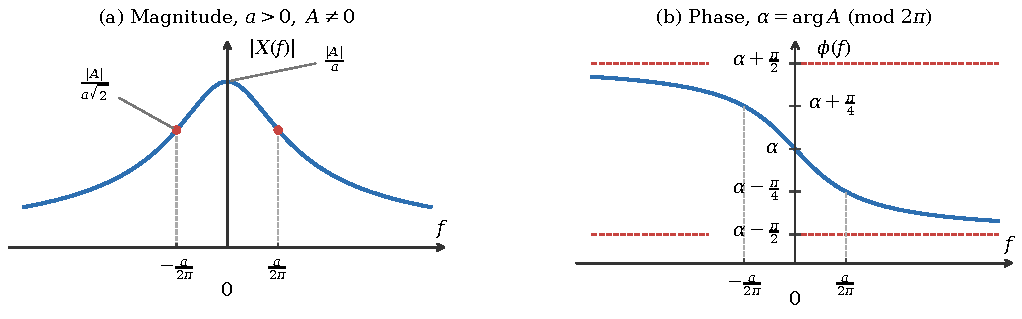
\includegraphics[width=.98\linewidth]{hw02-exponential.pdf}
\end{center}


\subsection*{本题知识点与公式}
\label{kn:2-2}
\begin{focusbox}{已学前置与本题新增}
强度、能量和频率单位见第\ref{kn:2-1}题。本题首次建立复数幅相、傅里叶变换、实信号频谱对称性以及时间尺度与谱宽的关系。后续的频移、调制和系统频响都使用这些约定。
\end{focusbox}

\subsubsection*{1. 复数的幅值与相位：频谱计算的基本工具}
用 $\iu^2=-1$，将复数写成直角坐标与极坐标形式
\[
z=p+\iu q=|z|e^{\iu\phi},\quad |z|=\sqrt{p^2+q^2},\quad
\phi=\operatorname{atan2}(q,p),\quad z^*=p-\iu q.
\]
双参数反正切保留象限；只用 $\arctan(q/p)$ 会把 $p<0$ 的象限弄错。$z=0$ 时相位无定义，非零复数的相位相差 $2\pi k$ 表示同一点。
\[
|z_1z_2|=|z_1||z_2|,\quad
\arg(z_1z_2)=\arg z_1+\arg z_2,
\]
\[
\left|\frac{z_1}{z_2}\right|=\frac{|z_1|}{|z_2|},\quad
\arg\frac{z_1}{z_2}=\arg z_1-\arg z_2\qquad(z_2\ne0).
\]
乘除运算可对模相乘除、相位相加减；加减运算却须先合并实虚部。通常 $|z_1+z_2|\ne|z_1|+|z_2|$，这正是第4、5题不能把两个幅谱直接相加的原因。

欧拉公式把振荡与复指数联系起来：
\[
e^{\iu\theta}=\cos\theta+\iu\sin\theta,\quad
\cos\theta=\frac{e^{\iu\theta}+e^{-\iu\theta}}2,\quad
\sin\theta=\frac{e^{\iu\theta}-e^{-\iu\theta}}{2\iu}.
\]
复指数 $e^{(\sigma+\iu\omega)t}$ 中，$\sigma$ 决定包络的增长/衰减，$\omega$ 决定振荡；两者都必须使指数的整体无量纲。

\subsubsection*{2. 傅里叶变换描述的是频率组成}
以 Hz 为变量的变换和反变换为
\[
X(f)=\int_{-\infty}^{\infty}x(t)e^{-\iu2\pi ft}\diff t,
\qquad x(t)=\int_{-\infty}^{\infty}X(f)e^{\iu2\pi ft}\diff f.
\]
幅谱 $|X(f)|$ 与相谱 $\arg X(f)$ 共同决定信号；一般不能只保留幅谱就重建原波形。对普通非周期可积信号，$X(f)$ 是连续频谱密度：若 $x$ 的单位为 V，则 $X(f)$ 的单位为 $\mathrm{V\,s}$，不是单个正弦的峰值电压。

$\int|x(t)|\diff t<\infty$ 是普通变换存在的常用充分条件，并非必要条件；在合适的分段光滑等条件下，反变换在连续点给出原值，在跳变点给出左右极限的平均值。若 $X$ 不绝对可积，反变换积分按对称截断极限 $\lim_{F\to\infty}\int_{-F}^{F}$ 理解。本题在 $t=0$ 有跳变，反演得到 $A/2$，而原题端点取 $A$；这个单点差异不改变频谱。常数、无限长正弦和阶跃不满足绝对可积条件，需要下一题的广义变换。

若以角频率 $\Omega$ 为变量，则
\[
X_\Omega(\Omega)=\int x(t)e^{-\iu\Omega t}\diff t=X\!\left(\frac\Omega{2\pi}\right),\qquad
x(t)=\frac1{2\pi}\int X_\Omega(\Omega)e^{\iu\Omega t}\diff\Omega.
\]
同一频率位置的连续谱数值只是换横坐标，反变换测度却有 $\diff\Omega=2\pi\diff f$。冲激谱还需结合冲激缩放律，不能只替换箭头位置；该点在第\ref{kn:2-3}题正式说明。

\subsubsection*{3. 首次用到的基本性质与检查方法}
下列等式默认变换以 $f$ 为变量，且信号满足普通或相应广义变换条件：
\begin{align*}
c_1x_1(t)+c_2x_2(t)&\longleftrightarrow c_1X_1(f)+c_2X_2(f),&&\text{线性},\\
x(t-t_d)&\longleftrightarrow X(f)e^{-\iu2\pi ft_d},&&\text{时移},\\
x(bt)&\longleftrightarrow\frac1{|b|}X\!\left(\frac fb\right),\ b\ne0,&&\text{时标伸缩},\\
x^*(t)&\longleftrightarrow X^*(-f),&&\text{共轭}.
\end{align*}
线性使复杂信号可拆成基本信号；时移仅改变相位，不改变幅谱；时间压缩会使频谱展宽，并改变谱密度的高度。若积分有意义，$X(0)=\int x(t)\diff t$，零频值可用时域面积核查；本题应为 $A/a$。

实信号满足共轭对称 $X(-f)=X^*(f)$：实部为偶函数、虚部为奇函数，幅谱为偶函数，相位可按模 $2\pi$ 取反。实偶信号的频谱为实偶函数，实奇信号的频谱为纯虚奇函数；相位不是简单地等于“虚部”。本题当 $A$ 为实数时适用这些实信号结论；若 $A$ 为一般复数，不能直接强加共轭对称。

对有限能量信号，帕塞瓦尔关系为（普通变换不收敛时，$X$ 按均方意义定义）
\[
\int|x(t)|^2\diff t=\int|X(f)|^2\diff f
=\frac1{2\pi}\int|X_\Omega(\Omega)|^2\diff\Omega.
\]
它连接时域能量与频域能量，$|X|^2$ 是能量谱密度，不是周期功率信号中冲激频谱的平方。

\subsubsection*{4. 单边指数的时间尺度与频谱特征}
因 $t<0$ 为零，本题应写 $Ae^{-at}u(t)$，其中 $a$ 的单位是 $\mathrm{s^{-1}}$。时间常数 $\tau_e=1/a$ 表示指数包络在 $t=\tau_e$ 时降至初值的 $e^{-1}$。由答案
\[
\frac{|X(f)|}{|X(0)|}=\frac1{\sqrt{1+(2\pi f/a)^2}},\quad
f_b=\frac a{2\pi},\quad E_x=\frac{|A|^2}{2a}.
\]
$f_b$ 处幅值为零频值的 $1/\sqrt2$，幅值平方为一半；在很高频率下 $|X(f)|\sim|A|/(2\pi|f|)$。$a$ 增大使衰减更快、归一化频谱更宽，但零频高度 $|A|/a$ 更低。此结论描述同一信号的时频对应，尚不等于已经给定某个测量系统的传递函数。


\nt{
    \textbf{易错：单边指数信号的负时间区间为零；横轴单位必须统一。}
    若去掉 $u(t)$，把 $Ae^{-at}$ 定义在全时间轴上，
    它在 $t\to-\infty$ 时发散，
    上述普通傅里叶积分不成立。
    用谱角频率写时为 $A/(a+\iu\Omega)$，
    改用 $f$ 后必须代入 $\Omega=2\pi f$。
    当 $A$ 为负实数时，可取 $\alpha=\pi$，再按所需主值区间折回相位；
    $A=0$ 时相位没有定义。
}

\needspace{11\baselineskip}
\section{第3题：符号函数与单位阶跃函数的广义频谱}
\label{hw:2-3}
\keypoint{复习重点：微分性质、冲激项、主值分布及其谱图表示。}

\begin{hwquestion}
求 $\sgn(t)$ 与 $u(t)$ 的频谱，
    使用频率 $f$ 为横坐标绘制幅频图与相频图。
    采用 $\sgn(0)=0$、$u(0)=1/2$ 的对称约定。
\end{hwquestion}

\subsection*{答案与解析}
这两个信号不绝对可积，不能把普通积分当作收敛积分计算。
引入主值符号 $\PV$，用对称方式处理 $f=0$ 附近的奇性。
\textbf{以下变换等式在广义函数意义下成立。}

\subsubsection{符号函数：用微分性质确定连续部分}
\[
    \sgn(t)=
    \begin{cases}
        -1,&t<0,\\
        1,&t>0,
    \end{cases}
    \qquad
    \frac{\diff}{\diff t}\sgn(t)=2\delta(t).
\]
设 $S(f)=\mathcal F\{\sgn(t)\}$。由
$\mathcal F\{x'(t)\}=\iu2\pi fX(f)$、
$\mathcal F\{\delta(t)\}=1$ 得
\[
    \iu2\pi fS(f)=2.
\]
在 $f\neq0$ 时，$S(f)=1/(\iu\pi f)$。
微分式本身不能排除 $C\delta(f)$，因为 $f\delta(f)=0$；
但 $\sgn(t)$ 是实奇函数，其频谱必须为纯虚奇分布，
不能含偶的 $\delta(f)$ 项。因此
\[
    \boxed{\mathcal F\{\sgn(t)\}
    =\PV\!\left(\frac{1}{\iu\pi f}\right)}.
\]
也可用收敛信号验证这个结果。令
$s_\varepsilon(t)=\sgn(t)e^{-\varepsilon|t|}$，$\varepsilon>0$，则
\begin{align*}
    \mathcal F\{s_\varepsilon(t)\}
    &=\frac{1}{\varepsilon+\iu2\pi f}
      -\frac{1}{\varepsilon-\iu2\pi f} \\
    &=\frac{-\iu4\pi f}{\varepsilon^2+(2\pi f)^2}
      \xrightarrow[\varepsilon\downarrow0]{\text{广义极限}}
      \PV\!\left(\frac{1}{\iu\pi f}\right).
\end{align*}

\subsubsection{单位阶跃：由符号函数补齐零频冲激}
利用 $u(t)=[1+\sgn(t)]/2$ 与 $\mathcal F\{1\}=\delta(f)$，可得
\[
    \boxed{U(f)=\mathcal F\{u(t)\}
    =\frac12\delta(f)
      +\PV\!\left(\frac{1}{\iu2\pi f}\right)}.
\]
这里 $\delta(f)/2$ 来自阶跃的常值分量。
若只对 $u'(t)=\delta(t)$ 做变换，
得到 $\iu2\pi fU(f)=1$，会漏掉微分消去的零频项；
所以必须另外确定冲激的系数。

\subsubsection{如何画幅频与相频示意图}
对 $f\neq0$，频谱是通常的复数函数，因而可以写
\[
    |S(f)|=\frac{1}{\pi|f|},
    \qquad
    |U_{\mathrm c}(f)|=\frac{1}{2\pi|f|},
\]
其中 $U_{\mathrm c}$ 表示阶跃谱的连续部分。两者相位相同：
\[
    \phi(f)=
    \begin{cases}
        +\pi/2,&f<0,\\
        -\pi/2,&f>0.
    \end{cases}
\]

\begin{center}
    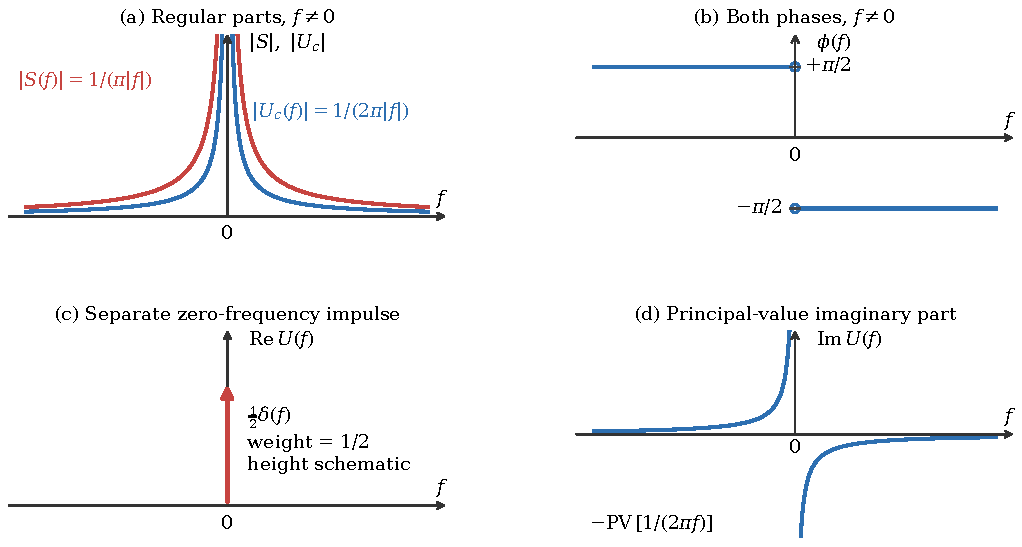
\includegraphics[width=.98\linewidth]{hw03-generalized.pdf}
\end{center}


\subsection*{本题知识点与公式}
\label{kn:2-3}
\begin{focusbox}{已学前置与本题新增}
复数幅相和变换约定见第\ref{kn:2-2}题。本题首次讲清冲激的权重、主值分布、微分/积分的变换性质，以及常数和正余弦线谱。核心是区分“普通函数在非零频率的值”与“整个广义频谱”。
\end{focusbox}

\subsubsection*{1. 单位冲激不是有限高度、零宽度的普通曲线}
冲激 $\delta(t)$ 由筛选作用定义：对适当连续的测试函数 $g$，
\[
\int_{-\infty}^{\infty}\delta(t-t_d)g(t)\diff t=g(t_d),\qquad
\int\delta(t)\diff t=1.
\]
因此 $c\delta(t-t_d)$ 的位置为 $t_d$、权重为 $c$；画谱时标注的是权重，而不是一个有限峰高。$\delta(t)$ 的量纲是 $\mathrm{s^{-1}}$，其积分才无量纲。与普通函数相乘时有
\[
g(t)\delta(t-t_d)=g(t_d)\delta(t-t_d),\qquad
t\delta(t)=0,\qquad \delta(bt)=\frac1{|b|}\delta(t)\quad(b\ne0).
\]
缩放式的绝对值来自保持积分权重不变。阶跃的广义导数为 $u'(t)=\delta(t)$；跳变大小为2的符号函数满足 $\sgn'(t)=2\delta(t)$。跳变点的单点赋值不改变这些关系。

\subsubsection*{2. 为什么要用主值，而不能直接计算 $1/f$ 在零点的值}
$1/f$ 在零点奇异，普通的左右两个反常积分均不收敛。取光滑且在无穷远快速衰减的测试函数 $g$，柯西主值采用对称删去零点附近区间后再取极限：
\[
\left\langle\PV\frac1f,g\right\rangle
=\lim_{\eta\downarrow0}\left(\int_{-\infty}^{-\eta}\frac{g(f)}f\diff f+
\int_{\eta}^{\infty}\frac{g(f)}f\diff f\right).
\]
尖括号表示分布对测试函数 $g$ 的作用。这定义了一种分布，而不是为 $f=0$ 人为指定一个数。$\PV(1/f)$ 与 $\delta(f)$ 作用方式不同：前者保留非零频率处的奇函数结构，后者只筛选零频处的信息。不能把主值奇性画成多余的冲激，也不能对含分布的整个表达式按普通复数直接取模或平方。

\subsubsection*{3. 微分性质为何不能唯一恢复零频项}
由分部积分，在端点项消失的条件下，
\[
\mathcal F\{x^{(n)}(t)\}=(\iu2\pi f)^nX(f).
\]
阶跃等信号须以广义函数意义使用。反过来求 $X$ 时，乘子 $f$ 会消去 $C\delta(f)$，所以除以 $f$ 后只能先确定非零频率部分。必须再用已知常数分量、奇偶性或原函数定义确定 $C$。本题符号函数的奇性排除偶冲激，而阶跃中的 $1/2$ 常数保留 $\delta(f)/2$。

把从负无穷积分写成与阶跃卷积，可得相应积分性质
\[
z(t)=\int_{-\infty}^{t}x(\lambda)\diff\lambda
\quad\longleftrightarrow\quad
Z(f)=\PV\frac{X(f)}{\iu2\pi f}+\frac{X(0)}2\delta(f),
\]
一个充分条件是 $x(t)$ 与 $t\,x(t)$ 都绝对可积，使 $X$ 在零点附近连续可微；等式按广义函数意义理解，不可直接对含未定义分布乘积的任意 $X$ 使用。最后一项不能随意省略；积分下限或积分常数改变，也可能改变直流冲激项。卷积的一般定义在第\ref{kn:2-4}题展开。

\subsubsection*{4. 应记住的广义变换对与正负频率相位}
在本册 Hz 约定下，$f_s>0$，有
\begin{align*}
\delta(t-t_d)&\longleftrightarrow e^{-\iu2\pi ft_d},\\
1&\longleftrightarrow\delta(f),\\
e^{\iu2\pi f_st}&\longleftrightarrow\delta(f-f_s),\\
\cos2\pi f_st&\longleftrightarrow\tfrac12[\delta(f-f_s)+\delta(f+f_s)],\\
\sin2\pi f_st&\longleftrightarrow\tfrac1{2\iu}[\delta(f-f_s)-\delta(f+f_s)].
\end{align*}
正余弦的谱线来自第\ref{kn:2-2}题的欧拉公式。正弦正频率的权重为 $-\iu/2$、负频率为 $+\iu/2$；两者的模均为 $1/2$，相位依次为 $-\pi/2$、$+\pi/2$。负频率是复指数相反的旋转方向，不是另一种独立的物理正弦。

本题两个重要变换对为
\[
\sgn(t)\longleftrightarrow\PV\frac1{\iu\pi f},\qquad
u(t)\longleftrightarrow\frac12\delta(f)+\PV\frac1{\iu2\pi f}.
\]
非零频率处均为纯虚数，$f>0$ 时为负虚数，故相位 $-\pi/2$；$f<0$ 时相位 $+\pi/2$。阶跃频谱的零频冲激需单独标注，不能把非零频率相位延伸到整个零频分布。

若改用角频率，利用 $\delta(\Omega/(2\pi)-f_s)=2\pi\delta(\Omega-2\pi f_s)$，可得
\[
\mathcal F_\Omega\{1\}=2\pi\delta(\Omega),\quad
\mathcal F_\Omega\{\cos\omega_st\}=\pi[\delta(\Omega-\omega_s)+\delta(\Omega+\omega_s)],
\]
\[
\mathcal F_\Omega\{u(t)\}=\pi\delta(\Omega)+\PV\frac1{\iu\Omega}.
\]
正是冲激缩放律使权重出现 $2\pi$；不能把 Hz 谱箭头平移到角频率横轴后仍保留原权重。


\nt{
    \textbf{易错：广义频谱不能在 $f=0$ 处直接取模。}
    图中的曲线仅表示 $f\neq0$ 的连续部分；
    阶跃谱在 $f=0$ 处还须单独画一个冲激箭头，标注\textbf{权重 $1/2$}。
    箭头长度不是有限的冲激高度，也不能把
    $|\delta(f)/2+1/(\iu2\pi f)|$ 当作普通函数计算。
    $f=0$ 的整个广义频谱不具有普通“幅值、相位”数值。
    符号函数的奇性是主值项，不能误画成额外的零频冲激。
}

\Needspace{11\baselineskip}
\section{第4题：截断余弦与两个平移的矩形窗频谱}
\label{hw:2-4}
\keypoint{复习重点：矩形窗变换、调制性质、幅频与有符号频谱的区别。}

\begin{hwquestion}
求
    \[
        y(t)=
        \begin{cases}
            \cos2\pi f_0t,&|t|\leq T,\\
            0,&|t|>T
        \end{cases}
    \]
    的傅里叶变换，并以 $f$ 为横坐标绘制频谱。
    其中 $T>0$，截断窗口总宽度为 $2T$。
\end{hwquestion}

\subsection*{答案与解析}
\textbf{先求窗谱，再搬移到 $\pm f_0$。}
令 $w(t)=1$（$|t|\leq T$），其余处为 $0$，则
$y(t)=w(t)\cos2\pi f_0t$。
\begin{align*}
    W(f)
    &=\int_{-T}^{T}e^{-\iu2\pi ft}\diff t \\
    &=\frac{e^{\iu2\pi fT}-e^{-\iu2\pi fT}}{\iu2\pi f}
      =\frac{\sin2\pi fT}{\pi f}
      =2T\Sa(2\pi fT).
\end{align*}
$f=0$ 处由极限补上 $W(0)=2T$。利用欧拉公式与频移性质：
\begin{align*}
    y(t)
    &=\frac12w(t)e^{\iu2\pi f_0t}
      +\frac12w(t)e^{-\iu2\pi f_0t},\\
    Y(f)
    &=\frac12W(f-f_0)+\frac12W(f+f_0).
\end{align*}
\[
    \boxed{Y(f)=T\Sa\bigl(2\pi T(f-f_0)\bigr)
       +T\Sa\bigl(2\pi T(f+f_0)\bigr)}.
\]
这也等价于把两条理想余弦谱线
$[\delta(f-f_0)+\delta(f+f_0)]/2$
分别与 $W(f)$ 卷积。

为绘制两个平移分量，记
\[
    Y_+(f)=T\Sa\bigl(2\pi T(f-f_0)\bigr),
    \qquad
    Y_-(f)=T\Sa\bigl(2\pi T(f+f_0)\bigr).
\]
下图分别画出 $Y_+(f)$ 和 $Y_-(f)$，竖线用于定位各自的中心频率。
$Y_+$ 在 $f=f_0$ 处峰高为 $T$，首零点为 $f_0\pm1/(2T)$；
$Y_-$ 在 $f=-f_0$ 处峰高为 $T$，首零点为 $-f_0\pm1/(2T)$。
这些峰和零点均属于\textbf{单个分量}；真正的总谱必须逐点代数相加：
$Y(f)=Y_+(f)+Y_-(f)$。

\begin{center}
    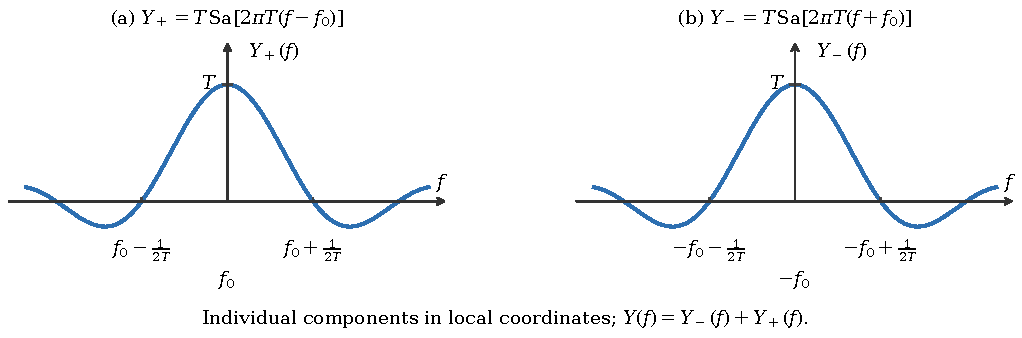
\includegraphics[width=.98\linewidth]{hw04-windowed.pdf}
\end{center}

\needspace{6\baselineskip}
\textbf{总频谱的幅值与相位。}
因为 $y(t)$ 为实偶函数，$Y(f)$ 也是实偶函数，
但其旁瓣可取负值。
幅频图应画 $|Y(f)|$；有符号的频谱图则保留负旁瓣。相位为
\[
    \phi(f)=
    \begin{cases}
        0,&Y(f)>0,\\
        \pi\quad(\mathrm{mod}\ 2\pi),&Y(f)<0,
    \end{cases}
\]
$Y(f)=0$ 处相位无定义。

\begin{center}
    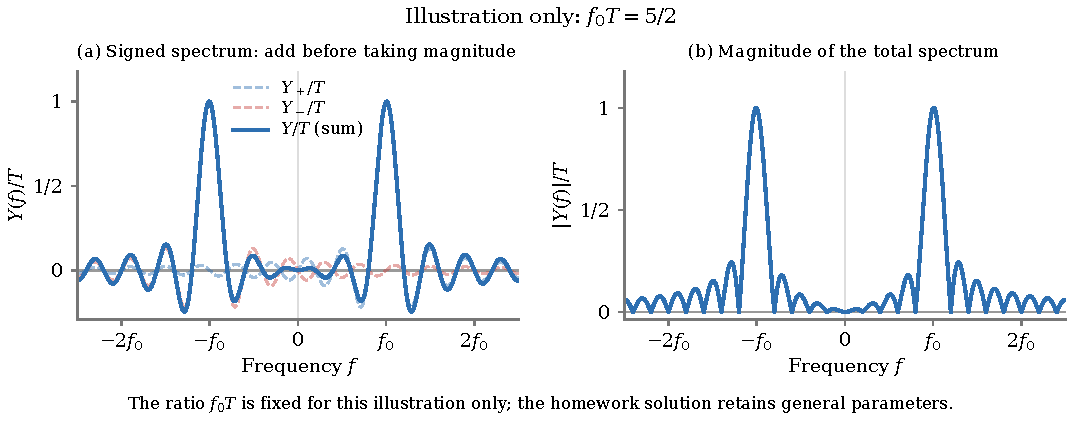
\includegraphics[width=.98\linewidth]{homework-windowed-total.pdf}
\end{center}
上图仅取 $f_0T=5/2$ 展示两个分量的代数相加与取模，未给原题增添已知条件；横轴为频率 $f$，纵轴除以 $T$ 归一化。左图保留总谱的正负旁瓣，右图为总幅谱。其他 $f_0T$ 比值的谱形由前述通式确定。


\subsection*{本题知识点与公式}
\label{kn:2-4}
\begin{focusbox}{已学前置与本题新增}
变换、复数叠加见第\ref{kn:2-2}题，余弦的冲激线谱见第\ref{kn:2-3}题。本题首次系统讲频移、卷积、时域相乘、矩形窗与主旁瓣。核心操作顺序是“构造复频谱，再相加，最后取模”。
\end{focusbox}

\subsubsection*{1. 频移性质与时移性质必须分开}
将指数乘子直接代入变换定义，可得
\[
\mathcal F\{x(t)e^{\iu2\pi f_ct}\}
=\int x(t)e^{-\iu2\pi(f-f_c)t}\diff t=X(f-f_c).
\]
所以频域的 $f-f_c$ 表示向右移动 $f_c$，$f+f_c$ 表示向左移动 $f_c$。利用欧拉公式，
\begin{align*}
x(t)\cos2\pi f_ct&\longleftrightarrow\tfrac12[X(f-f_c)+X(f+f_c)],\\
x(t)\sin2\pi f_ct&\longleftrightarrow\tfrac1{2\iu}[X(f-f_c)-X(f+f_c)].
\end{align*}
余弦为两个副本相加，正弦为复数副本相减。对照第\ref{kn:2-2}题，$x(t-t_d)$ 引入的是频域相位因子，既不搬动幅谱，也不产生这两个副本。

\subsubsection*{2. 卷积的定义、筛选作用与乘积定理}
时域卷积定义为
\[
(x*h)(t)=\int_{-\infty}^{\infty}x(\lambda)h(t-\lambda)\diff\lambda.
\]
它把各时刻 $x(\lambda)$ 对延迟响应 $h(t-\lambda)$ 的贡献累加；一般不是逐点乘积。频域卷积同理定义为
\[
(X*H)(f)=\int_{-\infty}^{\infty}X(\nu)H(f-\nu)\diff\nu.
\]
交换、结合和分配关系在适当的收敛条件下成立。冲激的筛选作用给出 $X(f)*\delta(f-f_c)=X(f-f_c)$，因而与冲激线谱卷积恰好产生频移。

在 Hz 变换约定下，两条成对性质为
\[
x(t)*h(t)\longleftrightarrow X(f)H(f),\qquad
x(t)h(t)\longleftrightarrow X(f)*H(f).
\]
第二式可把一个因子的反变换代入积分，并交换积分顺序推得。本题属于第二式：矩形窗与余弦在时域相乘，频域中窗谱与两条余弦冲激卷积。角频率约定下，时域乘积的频域卷积前须有 $1/(2\pi)$；不同约定不可混用。

\subsubsection*{3. 矩形窗、Sa与sinc的宽度约定}
记 $\operatorname{rect}(v)=1$（$|v|<1/2$），外部为零；端点定义不影响积分。若观察总时长为 $L$，则
\[
w_L(t)=\operatorname{rect}\!\left(\frac tL\right),\qquad
W_L(f)=L\Sa(\pi Lf)=L\operatorname{sinc}(Lf),
\]
其中 $\Sa z=\sin z/z$，归一化 $\operatorname{sinc}v=\sin(\pi v)/(\pi v)$，两者的自变量不同。$W_L(0)=L$，非零零点为 $f=k/L$（整数 $k\ne0$）。中心两侧首零点为 $\pm1/L$，主瓣零点间宽度为 $2/L$；其余振荡瓣称旁瓣。

本题 $L=2T$，所以 $W(f)=2T\Sa(2\pi Tf)$。乘以余弦后，两个副本各乘 $1/2$，分别以 $\pm f_0$ 为中心；各自的峰高 $T$、首零点偏移 $1/(2T)$、主瓣宽度 $1/T$ 都由此得出。它们是\textbf{各个分量}的属性，不保证就是总谱的峰高、峰位和零点。总谱仍满足
\[
Y(0)=2T\Sa(2\pi f_0T),\qquad
Y(f_0)=T[1+\Sa(4\pi f_0T)].
\]

\subsubsection*{4. 为什么截断产生泄漏，延长观察时间有什么作用}
无限长余弦的全部频率组成集中于 $\pm f_0$ 两条线；有限时长观察相当于加窗，窗谱把每条线展宽，并产生延伸到远处的旁瓣，这叫频谱泄漏。矩形窗的尾部只按约 $1/|f|$ 衰减，因而严格时限不等于严格带限。

增大 $L$ 会使首零点间距缩小，改善区分相近频率成分的能力；同时连续谱密度的峰高随 $L$ 增长，不能把这个增长误认为原余弦的时域峰值改变。窗函数的主瓣宽度与旁瓣大小存在折中：平滑端点通常能降低远旁瓣，却会改变主瓣宽度，具体指标应由所用窗计算，不能沿用矩形窗的零点公式。

本题的实偶时域信号使总谱为实偶，但负旁瓣仍代表相位 $\pi$；画有符号谱保留负值，画幅谱才取绝对值。先把旁瓣绝对化再叠加，会失去相消与相位信息，得到另一幅错误的谱。


\nt{
    \textbf{易错：截断并未保留两条理想谱线。}
    时域相乘对应频域卷积，有限窗口把谱线展宽为带旁瓣的连续谱。
    $T$ 是半窗宽，窗口频谱为 $2T\Sa(2\pi fT)$，
    不能误写成 $T\Sa(\pi fT)$。
    窗越长，主瓣越窄；两个平移的窗谱需要先做\textbf{代数相加}，
    再取绝对值，不能把两个窗谱的模直接相加。
    两端点取不取等号不影响傅里叶积分。
}

\needspace{11\baselineskip}
\section{第5题：指数衰减振荡的频谱与实际峰位}
\label{hw:2-5}
\keypoint{复习重点：指数谱频移、复数合并与幅频峰的位置。}

\begin{hwquestion}
原题为 $x(t)=e^{-at}\sin\omega t$。结合第2题，按 $a>0$、$\omega>0$ 且 $t\geq0$ 的单边衰减振荡解释，即
    $x(t)=e^{-at}\sin\omega t\,u(t)$。
    利用单边指数信号的频谱及傅里叶变换性质，求其频谱，
    并以 $f$ 为横坐标绘制幅频图。
\end{hwquestion}

\subsection*{答案与解析}
令 $g(t)=e^{-at}u(t)$，单边指数信号的变换为
$G(f)=1/(a+\iu2\pi f)$。
设振荡频率 $f_{\mathrm s}=\omega/(2\pi)$，由
$\sin\omega t=(e^{\iu\omega t}-e^{-\iu\omega t})/(2\iu)$ 得
\begin{align*}
    X(f)
    &=\frac{1}{2\iu}\bigl[G(f-f_{\mathrm s})-G(f+f_{\mathrm s})\bigr]\\
    &=\frac{1}{2\iu}
      \left[
        \frac{1}{a+\iu(2\pi f-\omega)}
        -\frac{1}{a+\iu(2\pi f+\omega)}
      \right]\\
    &=\boxed{\frac{\omega}{(a+\iu2\pi f)^2+\omega^2}}.
\end{align*}
把分母分成实部和虚部，得到幅频表达式
\[
    \boxed{
    |X(f)|=
    \frac{\omega}
    {\sqrt{\bigl[a^2+\omega^2-(2\pi f)^2\bigr]^2
    +4a^2(2\pi f)^2}}
    }.
\]
该幅值是偶函数，零频处为
$|X(0)|=\omega/(a^2+\omega^2)$。

\subsubsection*{幅谱峰位的推导}
令 $q=(2\pi f)^2\geq0$。幅值最大等价于其分母平方最小：
\begin{align*}
    D(q)
    &=(a^2+\omega^2-q)^2+4a^2q\\
    &=q^2+2(a^2-\omega^2)q+(a^2+\omega^2)^2,\\
    D'(q)&=2(q+a^2-\omega^2).
\end{align*}
因此，
\[
    \boxed{
    f_{\mathrm{peak}}=
    \begin{cases}
        \displaystyle\pm\frac{\sqrt{\omega^2-a^2}}{2\pi},
            &\omega>a,\\[2mm]
        0,&0<\omega\leq a.
    \end{cases}}
\]
当 $\omega>a$ 时，存在两个对称峰，峰高为 $1/(2a)$；
当 $\omega\leq a$ 时，最大值在中心，峰高为
$\omega/(a^2+\omega^2)$。
弱衰减 $a\ll\omega$ 时，双峰才接近 $\pm\omega/(2\pi)$。


绘制幅谱时，先标出中心值 $\omega/(a^2+\omega^2)$、上述峰位和峰高，
再利用关于纵轴的对称性补齐曲线。
下图分别示意 $\omega>a$ 的双峰与 $0<\omega\leq a$ 的中心单峰。

\begin{center}
    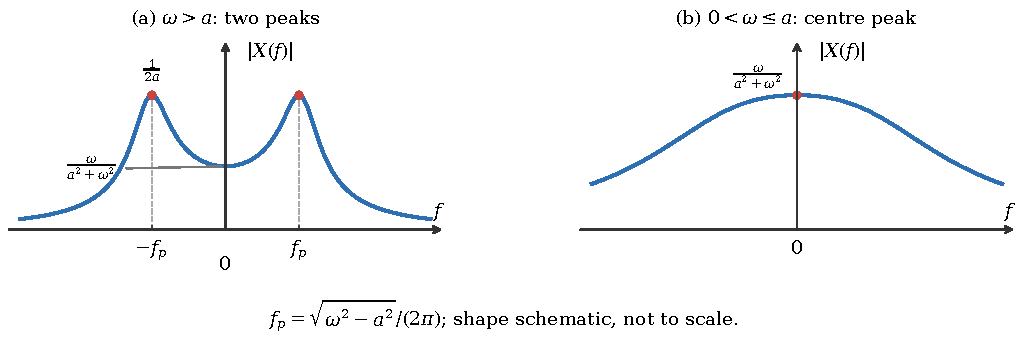
\includegraphics[width=.98\linewidth]{hw05-damped.pdf}
\end{center}


\subsection*{本题知识点与公式}
\label{kn:2-5}
\begin{focusbox}{已学前置与本题新增}
指数谱见第\ref{kn:2-2}题，正弦线谱和频移见第\ref{kn:2-3}、\ref{kn:2-4}题。本题新增单边阻尼振荡的包络、谱相位、能量，以及“振荡频率”和“幅谱峰位”之间的区别；变换性质本身不再重复推导。
\end{focusbox}

\subsubsection*{1. 衰减率与振荡频率控制不同的时间特征}
对 $e^{-at}\sin\omega t\,u(t)$，$a>0$ 的单位为 $\mathrm{s^{-1}}$，$\omega>0$ 的单位为 $\mathrm{rad/s}$。指数包络为 $\pm e^{-at}$，包络时间常数为 $1/a$；正弦因子的振荡周期为 $T_s=2\pi/\omega$，每经过一个振荡周期，包络比值为
\[
\frac{e^{-a(t+T_s)}}{e^{-at}}=e^{-2\pi a/\omega}.
\]
因此 $a/\omega$ 是判断衰减相对振荡快慢的无量纲量。整个信号不是周期信号，尽管其中的正弦因子有周期。乘上 $u(t)$ 又破坏了整条时间轴上的奇对称，不能因为含正弦便断言其频谱纯虚。

\subsubsection*{2. 两个复数副本相减后，幅值与相位怎样提取}
第\ref{kn:2-4}题的正弦调制公式给出两个指数谱的差；合并后设
\[
X(f)=\frac{\omega}{D_R(f)+\iu D_I(f)},\quad
D_R=a^2+\omega^2-(2\pi f)^2,\quad D_I=4\pi af.
\]
由于分子为正实数，相位为
\[
\phi(f)=-\operatorname{atan2}\!\left(4\pi af, a^2+\omega^2-(2\pi f)^2\right).
\]
零频处相位为零；当正频率足够大时，分母实部为负、虚部为正，输出相位趋于 $-\pi$，不能用普通反正切误画成回到零。负频率相位按共轭对称取反；幅谱始终为偶函数。这里 $X(f)$ 没有有限频率零点，因为 $\omega>0$ 且分母对实 $f$ 不为零。

谱峰位置由分母模的极小值决定，不能只看频移中心。答案已经给出 $\omega>a$ 时的双峰 $\pm\sqrt{\omega^2-a^2}/(2\pi)$ 与 $\omega\leq a$ 时的中心峰。弱衰减条件下可展开为
\[
f_{\mathrm{peak},+}=\frac{\omega}{2\pi}\sqrt{1-\frac{a^2}{\omega^2}}
\approx\frac{\omega}{2\pi}\left(1-\frac{a^2}{2\omega^2}\right),\qquad a/\omega\ll1.
\]
这个近似说明峰位接近正弦频率需要额外条件，不是频移公式自动保证的结论。

\subsubsection*{3. 用能量和高频渐近检查频谱}
由 $\sin^2\omega t=(1-\cos2\omega t)/2$ 及指数积分，
\begin{align*}
E_x&=\int_0^\infty e^{-2at}\sin^2\omega t\diff t\\
&=\frac1{4a}-\frac{a}{4(a^2+\omega^2)}
=\frac{\omega^2}{4a(a^2+\omega^2)}.
\end{align*}
本题是有限能量信号，平均功率为零，帕塞瓦尔关系可据此检查 $\int|X(f)|^2\diff f$。在 $|f|\to\infty$ 时，
\[
|X(f)|\sim\frac{\omega}{(2\pi f)^2}.
\]
其高频衰减比第2题的 $1/|f|$ 更快：本题在 $t=0$ 连续且为零，而单边指数在零点有幅值跳变；时域边界的光滑性会影响频域尾部。不能据此取消本题的单边条件，也不能把它替换为双边 $e^{-a|t|}\sin\omega t$，那是另一个信号。

\nt{
    \textbf{易错：两次频移后的复数谱要先相减，再取模。}
    不能把 $|X(f)|$ 画成两个指数幅频图的简单叠加，
    也不能因正弦的名义频率是 $\omega$ 就把最大值固定在 $\pm\omega$。
    这里横轴为 $f$，频率位置均须除以 $2\pi$。
    若省略 $u(t)$ 而把原式定义在整条实轴上，
    负时间方向会指数增长，普通傅里叶积分不收敛。
}

\needspace{11\baselineskip}
\section{第6题：余弦调制与频谱搬移、重叠}
\label{hw:2-6}
\keypoint{复习重点：欧拉展开的 $1/2$ 系数、两个搬移副本及频带重叠条件。}

\begin{hwquestion}
原题中的时间函数记作 $f(t)$。为避免与频率变量 $f$ 混淆，以下将其改记为 $m(t)$，频谱为 $M(f)$，按原图采用实值带限模型
    \[
        M(f)=0\quad(|f|>f_m),
        \qquad f_m=\frac{\omega_m}{2\pi}>0.
    \]
    采用角频率为 $\omega_0>0$ 的余弦载波，记
    \[
        f_{\mathrm c}=\frac{\omega_0}{2\pi},
        \qquad s(t)=m(t)\cos\omega_0t.
    \]
    求调幅信号 $s(t)$ 的傅里叶变换，示意画出时域和频域信号，
    并讨论 $\omega_0>\omega_m$、$\omega_0=\omega_m$
    与 $\omega_0<\omega_m$ 时的频带关系。
\end{hwquestion}

\subsection*{答案与解析}
利用欧拉公式展开载波，再应用频移性质：
\begin{align*}
    s(t)
    &=\frac12m(t)e^{\iu2\pi f_{\mathrm c}t}
      +\frac12m(t)e^{-\iu2\pi f_{\mathrm c}t}.
\end{align*}
\[
    \boxed{S(f)=\frac12M(f-f_{\mathrm c})
        +\frac12M(f+f_{\mathrm c})}.
\]
两项分别把原谱搬到正、负载频处，
每个副本都乘 $1/2$，谱形保持不变。
若改用谱角频率 $\Omega$ 为横轴，定义
$\mathcal M(\Omega)=M(\Omega/2\pi)$、
$\mathcal S(\Omega)=S(\Omega/2\pi)$，则同一结论写作
\[
    \boxed{\mathcal S(\Omega)
      =\frac12\mathcal M(\Omega-\omega_0)
       +\frac12\mathcal M(\Omega+\omega_0)}.
\]

\subsubsection{时域图：快速振荡受调制信号控制}
对于实信号，$|s(t)|\leq|m(t)|$ 始终成立。
在本题严格带限且 $f_c>f_m$ 的谱分离条件下，可先画 $m(t)$ 的形状，再在其内部画载波振荡，解析幅值包络为 $|m(t)|$；若 $m(t)\geq0$，上下包络为 $\pm m(t)$。$m(t)$ 变号时还会使载波翻转 $\pi$ 相位。若载频过低、两谱副本重叠，则 $\pm|m(t)|$ 仍提供逐点幅值界，但一般不再等于解析包络。
该调制信号没有额外的常值载波项，
是双边带抑制载波调制的基本形式。

下图根据给定的 $m(t)$ 轮廓，在包络内画出载波振荡，
并将一般的 $M(f)$ 轮廓左右平移以构造调制频谱。
时域包络与频谱轮廓为形状示意；
频带端点和每个副本的 $1/2$ 系数由变换公式决定。

\begin{center}
    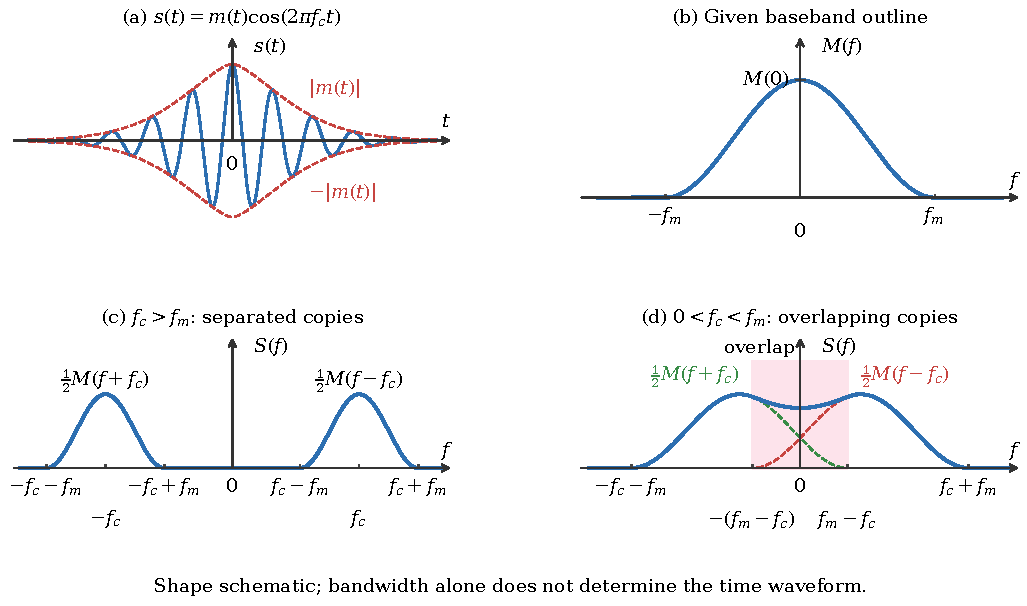
\includegraphics[width=.98\linewidth]{hw06-modulation.pdf}
\end{center}


\subsection*{本题知识点与公式}
\label{kn:2-6}
\begin{focusbox}{已学前置与本题新增}
频移和卷积见第\ref{kn:2-4}题，冲激线谱见第\ref{kn:2-3}题。本题新增基带、载波、边带和带宽的完整含义，频带重叠与相干解调，并补齐后续多频应变和调幅题需要的傅里叶级数与谱线幅值约定。
\end{focusbox}

\subsubsection*{1. 基带、载波、边带及带宽应怎样定义}
$m(t)$ 携带被测信息，称调制信号，其未经搬移的频谱称基带谱；$\cos2\pi f_ct$ 为载波，$s(t)$ 为已调信号。本题是乘法调制：信息改变高频振荡的幅值及正负符号。严格带限模型 $M(f)=0$（$|f|>f_m$）中，$f_m$ 为基带最高频率；基带正频率带宽为 $f_m$，不要把双边支撑区间的宽度 $2f_m$ 也叫同一个基带带宽。

调制的两个副本支撑在
\[
I_+=[f_c-f_m,f_c+f_m],\qquad I_-=[-f_c-f_m,-f_c+f_m].
\]
当 $f_c>f_m$，正载频附近的双边带占用宽度为 $B=2f_m$，上下边带分别位于载频两侧。两个副本间隔为 $2(f_c-f_m)$；$f_c=f_m$ 时在零频相接；$0<f_c<f_m$ 时交集为
\[
I_+\cap I_-=[-(f_m-f_c),\ f_m-f_c],
\]
重叠宽度 $2(f_m-f_c)$。若原谱内部有空隙或端点为零，上述区间只是可能支撑的范围；发生实际相加仍取决于两个副本在该频率处是否非零。实际非严格带限信号只能按规定的有效带宽作近似判断。

\subsubsection*{2. 抑制载波、包络与有符号信息}
本题 $s=m\cos2\pi f_ct$ 没有额外的常值载波项，称双边带抑制载波调制。若 $m$ 自身含直流 $D$，则 $D\cos2\pi f_ct$ 仍会产生载波线，不能仅凭写成乘积就断言载波处一定无线谱。对一般连续基带谱，频移也不凭空产生独立冲激。

在上述严格带限且 $f_c>f_m$ 的条件下，幅值包络为 $|m(t)|$；若 $m$ 变号，载波还翻转 $\pi$ 相位。对实际有效带限、载波远快于包络的情况，这可作近似解释。只测包络会丢失这个符号。带直流偏置的常规调幅 $[D+m(t)]\cos2\pi f_ct$ 可在频谱分离、$D+m(t)$ 不变号时用包络恢复偏置后的信号；具体多音条件在第\ref{kn:5-3}题展开。

\subsubsection*{3. 同步相乘为什么能把信息搬回低频}
将 $s(t)$ 乘同频参考 $\cos(2\pi f_ct+\theta_r)$，积化和差给出
\[
s(t)\cos(2\pi f_ct+\theta_r)
=\frac12m(t)\cos\theta_r+
\frac12m(t)\cos(4\pi f_ct+\theta_r).
\]
第一项回到基带，第二项移至 $2f_c$ 附近。低通滤波是保留低频、抑制高频的操作；若其通带覆盖 $|f|\leq f_m$，又能抑制 $2f_c$ 附近的项，则输出为 $m(t)\cos\theta_r/2$。同相时乘2可恢复原信号；相差 $90^\circ$ 时理想基带输出为零，故参考的频率与相位都重要。

$f_c>f_m$ 保证基带上端 $f_m$ 低于高频项下端 $2f_c-f_m$，为理想滤波分离提供空隙。若两个搬移副本重叠，同一变换公式仍成立，但简单带通分离以及上述直接低通恢复条件可能失效；这与离散采样造成的混叠不是同一个操作，也不等于在附加信息下任何方法都无法恢复。

\subsubsection*{4. 周期多频信号：傅里叶级数与三角系数}
后续应变和调幅题常给出多个正弦之和。对周期为 $T_0$、基角频率 $\omega_0=2\pi/T_0$ 的实信号，采用常数项直接记作 $a_0$ 的约定：
\[
x(t)=a_0+\sum_{n=1}^\infty[a_n\cos n\omega_0t+b_n\sin n\omega_0t],
\]
\[
a_0=\frac1{T_0}\int_{t_*}^{t_*+T_0}x(t)\diff t,\quad
a_n=\frac2{T_0}\int_{t_*}^{t_*+T_0}x(t)\cos n\omega_0t\diff t,
\]
\[
b_n=\frac2{T_0}\int_{t_*}^{t_*+T_0}x(t)\sin n\omega_0t\diff t.
\]
这些系数来自不同整数次正弦、余弦在一个周期上的正交性。例如对正整数 $n,m$，
\[
\int_{t_*}^{t_*+T_0}\cos n\omega_0t\cos m\omega_0t\diff t
=\begin{cases}0,&n\ne m,\\T_0/2,&n=m.\end{cases}
\]
正弦与正弦同理，正弦与余弦的交叉积分为零。将展开式乘某一基函数再积分，只留下对应项，所以非零频率系数前有 $2/T_0$。另一常见写法把常数项记作 $a_0/2$，此时常数系数定义相应改变，不能混用。分段光滑等充分条件下，级数在连续点收敛到原值，在跳变点收敛到左右极限平均值。

三角项可合并为单个余弦：
\[
a_n\cos n\omega_0t+b_n\sin n\omega_0t
=A_n\cos(n\omega_0t-\theta_n),
\]
\[
A_n=\sqrt{a_n^2+b_n^2},\qquad \theta_n=\operatorname{atan2}(b_n,a_n).
\]
若 $A_n=0$，该项相位不定义。实偶信号使 $b_n=0$，实奇信号使 $a_0=a_n=0$，可在积分前简化计算。

\subsubsection*{5. 复指数系数、单边峰值与双边冲激权重}
同一周期信号还可写为
\[
x(t)=\sum_{n=-\infty}^{\infty}C_ne^{\iu n\omega_0t},\qquad
C_n=\frac1{T_0}\int_{t_*}^{t_*+T_0}x(t)e^{-\iu n\omega_0t}\diff t.
\]
对实信号，$C_0=a_0$，$C_n=(a_n-\iu b_n)/2$（$n>0$），$C_{-n}=C_n^*$，故 $|C_{\pm n}|=A_n/2$。$C_n$ 与 $x$ 同单位；Hz 傅里叶变换为
\[
X(f)=\sum_n C_n\delta(f-nf_0),\qquad f_0=1/T_0.
\]
因此“时域余弦峰值”“复指数系数模”“角频率变换中的冲激权重的模”依次为 $A_n$、$A_n/2$、$\pi A_n$。对上式的 $A_n\cos(n\omega_0t-\theta_n)$，正角频率处实际复权重为 $2\pi C_n=\pi A_ne^{-\iu\theta_n}$，负频率处为其共轭；不能遗漏相位。这里的 $2\pi$ 来自第\ref{kn:2-3}题的冲激缩放。直流只在零频出现，不能也按正负频率分成两半。

一周期平方可积时，正交性还给出周期功率的帕塞瓦尔关系
\[
x_{\mathrm{rms}}^2=P_x=\sum_{n=-\infty}^{\infty}|C_n|^2
=a_0^2+\frac12\sum_{n=1}^\infty(a_n^2+b_n^2).
\]
它与第\ref{kn:2-1}题的有效值相连，便于计算多频信号的强度；频率不同、在共同周期正交的分量，均方值可以相加，峰值一般不能这样相加。对无限长周期信号，不应通过把冲激傅里叶谱直接平方来计算功率。


\nt{
    \textbf{易错：重叠区仍按同一变换公式计算，且系数始终为 $1/2$。}
    $\omega_0<\omega_m$ 不会使频移性质失效，
    只是两个副本在同一频率处发生叠加。
    “不能靠带通分离副本”也不等于“任何方法都无法恢复原信号”；
    恢复能力还取决于所用方法及信号的额外信息。
    时域相乘引起频域搬移，时域平移则引起相位因子，二者不可混用。
}

\chapter{测试系统的特性}
\label{hw:systems}

\noindent 本章对应《课后作业-CH3》的全部4题。数值答案以静态灵敏度标定后的输出为准，取归一化静态增益 $K=1$；相角差统一定义为“输出相位减输入相位”。知识说明中保留一般静态灵敏度 $K>0$；实际输出幅值需再乘 $K$，归一化幅值误差与相位结论不变。

\section{第1题：双频信号通过一阶装置}
\label{hw:3-1}
\begin{hwquestion}
求周期信号 $x(t)=0.5\cos(10t)+0.2\cos(100t-45^\circ)$ 通过传递函数
$H(s)=1/(0.005s+1)$ 的装置后得到的稳态响应。要求根据线性叠加特性和一阶系统动态特性计算，并分析不同频率的幅值、相位变化规律。
\end{hwquestion}

\subsection*{答案与解析}
由 $\tau=0.005\,\mathrm{s}$ 得
\[
H(\iu\omega)=\frac{1}{1+\iu0.005\omega},\qquad
A(\omega)=\frac{1}{\sqrt{1+(0.005\omega)^2}},\qquad
\phi(\omega)=-\arctan(0.005\omega).
\]
稳定线性时不变系统对每个正弦分量分别作“幅值乘 $A$、原相位加 $\phi$”的变换。两个分量的角频率为 $10$ 与 $100\,\mathrm{rad/s}$，于是
\begin{align*}
A_1&=(1+0.05^2)^{-1/2}=0.998752,
&\phi_1&=-\arctan0.05=-2.8624^\circ,\\
A_2&=(1+0.5^2)^{-1/2}=0.894427,
&\phi_2&=-\arctan0.5=-26.5651^\circ.
\end{align*}
因此 $y_1(t)=0.499376\cos(10t-2.8624^\circ)$，
$y_2(t)=0.178885\cos(100t-45^\circ-26.5651^\circ)$。叠加得
\[
\boxed{\begin{aligned}
y_{\mathrm{ss}}(t)\approx{}&0.499376\cos(10t-2.8624^\circ)\\
&+0.178885\cos(100t-71.5651^\circ).
\end{aligned}}
\]
相位中的度数是常相位的标注；用计算程序求值时须转为弧度。

\begin{center}
\small
\begin{tabular}{@{}ccccc@{}}
\toprule
$\omega/(\mathrm{rad/s})$ & 输入幅值 & 输出幅值 & 幅值衰减 & 系统相角差\\
\midrule
$10$ & $0.5$ & $0.499376$ & $0.1248\%$ & $-2.8624^\circ$\\
$100$ & $0.2$ & $0.178885$ & $10.5573\%$ & $-26.5651^\circ$\\
\bottomrule
\end{tabular}
\end{center}
频率升高时，一阶装置的幅值比单调降低，相位由 $0$ 向 $-90^\circ$ 滞后；输出各分量仍与各自输入同频。高频项受到更强衰减和更大相位滞后，故叠加后的波形发生变化。

\begin{focusbox}{知识主线}
把装置看成稳定线性时不变系统：由微分方程建立 $H(s)$，令 $s=\iu\omega$ 得到正弦稳态的幅值比与相位差，最后逐频叠加。下文依次解释这些步骤的依据，以及为什么同频输出仍可能改变多频波形。
\end{focusbox}

\subsection*{本题知识点与公式}
\label{kn:3-1}
\noindent\textbf{已学前置：}第\ref{kn:2-2}节的复数频谱、幅值与相位，第\ref{kn:2-4}节的卷积与时频域联系。
\textbf{本题新增：}系统的线性与时不变性、传递函数和初值条件、冲激响应、一阶模型、相量稳态法、稳态与暂态及不失真测量。

\subsubsection*{1. 为什么可以分开计算两项：线性、时不变与零状态}
用 $\mathcal T$ 表示装置对输入的作用。若在\textbf{零初始状态}下 $x_1\mapsto y_1$、$x_2\mapsto y_2$，线性要求对任意常数 $a,b$ 都有
\[
\mathcal T\{ax_1+bx_2\}=a\mathcal T\{x_1\}+b\mathcal T\{x_2\}.
\]
其中 $a\mathcal T\{x_1\}$ 是比例性，两种输入响应相加是叠加性。因此本题可以分别求两项的响应再相加。零状态意味着储能元件没有额外初始能量，例如电容初始电压或机械质量块初始位移、速度为零。存在初始能量时，还要单独加入它引起的零输入响应，不能把该响应重复加入每一项。

时不变性则要求输入整体延后 $t_0$，输出也仅延后相同时间：
\[
\mathcal T\{x(t-t_0)\}=y(t-t_0).
\]
常系数线性微分方程在相应的固定工作条件下给出典型的线性时不变（LTI）模型。线性与时不变是两项要求；调制环节 $y(t)=x(t)\cos\omega_ct$ 对输入线性，却因系数随时间变化而不是时不变系统，会搬移频率。\textbf{本题逐频保持原频率的结论依赖稳定LTI模型，而不只是“线性”二字。}实际装置发生饱和、明显迟滞或参数随工况变化时，应重新检查这一模型是否适用。

\subsubsection*{2. 从微分方程到传递函数：$H(s)$ 包含什么信息}
若输入 $x(t)$、输出 $y(t)$ 满足
\[
a_1\dot y(t)+a_0y(t)=b_0x(t),
\]
在 $a_0\ne0$ 时除以 $a_0$，令 $\tau=a_1/a_0$、$K=b_0/a_0$，就得到一阶标准模型
\[
\boxed{\tau\dot y+y=Kx},\qquad \tau>0.
\]
例如电阻、电容构成的低通电路满足 $RC\dot u_C+u_C=u_{\mathrm{in}}$，故 $\tau=RC$、$K=1$。机械、热学等装置的一个主要惯性过程也可能在限定工作范围内近似成相同形式；“一阶”指最高时间导数为一阶，并非指输入只有一个频率。

引入拉普拉斯变换 $X(s)=\int_{0^-}^{\infty}x(t)e^{-st}\diff t$，其中 $s=\sigma+\iu\omega$ 为复频率。用
$\mathcal L\{\dot y\}=sY(s)-y(0^-)$ 得
\[
(\tau s+1)Y(s)=KX(s)+\tau y(0^-).
\]
零初值时，输入输出之比定义为传递函数：
\[
\boxed{H(s)=\left.\frac{Y(s)}{X(s)}\right|_{\text{零初值}}
=\frac{K}{1+\tau s}}.
\]
它由装置参数及输入输出的选取决定，不随输入的具体波形改变。非零初值时，右端还存在 $\tau y(0^-)$，所以不能直接用 $Y=HX$ 代表总响应。更一般的常系数方程
$\sum_k a_k y^{(k)}=\sum_k b_k x^{(k)}$，在零初值下同样给出 $H(s)=\sum_k b_ks^k/\sum_k a_ks^k$。

符号和量纲要对应：$t,\tau$ 用秒，$s,\omega$ 用 $\mathrm{s}^{-1}$（角频率通常写 $\mathrm{rad/s}$），所以 $\tau s$ 和 $\omega\tau$ 无量纲。$K=H(0)$ 是静态增益或静态灵敏度，单位为“输出单位/输入单位”，不一定无量纲。例如输入力、输出电压时，$K$ 的单位是 $\mathrm{V/N}$。本题给出的模型相当于已归一化为 $K=1$。

\subsubsection*{3. 冲激响应与卷积：同一系统的时域描述}
单位冲激输入 $\delta(t)$ 所产生的零状态输出记为 $h(t)$，称冲激响应。冲激满足 $\int\delta(t)\diff t=1$，是“面积为1”的理想输入，而不是高度为1的窄脉冲。因果系统在冲激到达前没有输出，故 $h(t)=0$（$t<0$）。把输入分解为各时刻的冲激，再利用线性和时不变性，得到
\[
\boxed{y_{\mathrm{zs}}(t)=(h*x)(t)
=\int_{0}^{\infty}h(\xi)x(t-\xi)\diff\xi}.
\]
对从 $t=0$ 才接入的因果输入，积分上限可改为 $t$。这里 $\xi$ 为历史时间，$h$ 的单位是增益单位再除以秒，使积分后量纲仍为输出单位。卷积的频域联系见第\ref{kn:2-4}节。

一阶模型在 $t>0$ 的冲激响应满足 $\tau\dot h+h=0$；跨越 $t=0$ 对方程积分，得到 $\tau[h(0^+)-h(0^-)]=K$。结合因果性可得
\[
\boxed{h(t)=\frac{K}{\tau}e^{-t/\tau}u(t)},\qquad
H(s)=\mathcal L\{h(t)\}.
\]
当 $\tau>0$ 时，$h(t)$ 衰减且绝对可积，系统可建立稳定的正弦稳态。其傅里叶变换就是频率响应：
\[
H(\iu\omega)=\int_{-\infty}^{\infty}h(t)e^{-\iu\omega t}\diff t
=\frac{K}{1+\iu\omega\tau}.
\]
因此 $H(s)$、$h(t)$ 和 $H(\iu\omega)$ 分别从复频域、时域和正弦频率域描述同一LTI系统。不是任意传递函数都能通过令 $s=\iu\omega$ 就解释成稳定稳态响应；还要有适当的稳定性条件。本题极点 $s=-1/\tau<0$，自然响应会衰减，满足这一条件。

\subsubsection*{4. 相量法如何给出正弦稳态的幅值与相位}
把实余弦写成复指数的实部：
$x(t)=\Re\{\widehat X e^{\iu\omega t}\}$，其中 $\widehat X=X_0e^{\iu\theta}$ 为相量，$X_0\geq0$ 是输入峰值。设稳态输出为 $y_{\mathrm{ss}}=\Re\{\widehat Y e^{\iu\omega t}\}$。代入一阶方程，求导仅引入 $\iu\omega$，故
\[
(1+\iu\omega\tau)\widehat Y=K\widehat X,
\qquad \widehat Y=H(\iu\omega)\widehat X.
\]
复数相乘使模相乘、相角相加。因此对 $K>0$，定义归一化幅值比 $a(\omega)=|H(\iu\omega)|/K$，有
\[
a(\omega)=\frac{1}{\sqrt{1+(\omega\tau)^2}},\qquad
\phi(\omega)=\arg H(\iu\omega)=-\arctan(\omega\tau),
\]
\[
\boxed{y_{\mathrm{ss}}(t)=KX_0a(\omega)
\cos[\omega t+\theta+\phi(\omega)]}.
\]
若输入用正弦表示，输出也写正弦，仍使用相同的幅值比和相位差。相位差是输出相位减输入相位，负号表示滞后。$|H|$ 可能有单位，$a$ 无量纲；本题 $K=1$，答案中的 $A(\omega)$ 就等于这里的 $a(\omega)$。对于实际传感器，不能省去静态灵敏度就把伏特与牛顿等不同物理量直接比较大小。

\subsubsection*{5. 一阶响应为何包含稳态与暂态}
齐次方程 $\tau\dot y+y=0$ 的解为 $Ce^{-t/\tau}$。任意特解加上齐次解都满足原方程，所以从有限时刻开始测量时，总响应为
\[
y(t)=y_{\mathrm{ss}}(t)+Ce^{-t/\tau},\qquad
C=y(0^+)-y_{\mathrm{ss}}(0).
\]
前一项由持续输入决定，后一项调整初始条件。$\tau>0$ 时后一项随时间衰减，经过足够长时间只剩稳态。零初始状态并不等于“没有暂态”：即使 $y(0)=0$，为了满足启动条件也通常需要一个非零的 $C$。

若从静止开始施加阶跃 $x(t)=X_su(t)$，常值特解为 $KX_s$，配合 $y(0)=0$，得到
\[
y(t)=KX_s(1-e^{-t/\tau})\quad(t\geq0).
\]
这是同一个模型的阶跃响应；第\ref{kn:3-2}节将用它定义响应速度指标。稳态正弦与阶跃全过程并非两套互不相干的公式，而是同一微分方程在不同输入下的解。

\subsubsection*{6. 为什么同频不等于不失真}
对多频信号，逐项使用上述相量关系再叠加即可。若所有分量仅经历相同增益 $K_d$ 和共同时间延迟 $t_d$，则
\[
y(t)=K_dx(t-t_d),\qquad
H(\iu\omega)=K_de^{-\iu\omega t_d}
\]
必须在信号所占的频带内成立。这等价于该频带内幅频特性为常数、展开后的相频特性为通过原点的直线：
$|H(\iu\omega)|=K_d$、$\phi(\omega)=-\omega t_d$。不同频率的相位差应与频率成比例，而不是全部相等。

本题两项幅值比为 $0.998752$ 与 $0.894427$，其由相角换算的时间延迟约为 $4.996$ 与 $4.636\,\mathrm{ms}$，均不完全相同。因此每项虽然仍保持原频率，叠加波形却不再严格等于输入的整体放大、延后版本。工程中的“近似不失真”必须结合信号频带及允许的幅值、相位误差来判断；一阶装置在 $\omega\tau\ll1$ 的低频区更接近这一要求。
\nt{\textbf{易错点：}$10t$、$100t$ 中的系数是角频率，不能再乘 $2\pi$；第二项的系统相角差为 $-26.5651^\circ$，输出总相位为 $-71.5651^\circ$，两者不能混写。}

\needspace{11\baselineskip}
\section{第2题：由幅值误差反求时间常数}
\label{hw:3-2}
\begin{hwquestion}
用一阶系统测量 $100\,\mathrm{Hz}$ 正弦信号，要求振幅误差在 $5\%$ 以内，时间常数应取多少？若用该系统测量 $50\,\mathrm{Hz}$ 正弦信号，此时振幅误差和相角差是多少？要求写出所选系统的频响函数，并计算 $50\,\mathrm{Hz}$ 输入时的稳态输出。
\end{hwquestion}

\subsection*{答案与解析}
一阶系统 $H(s)=1/(1+\tau s)$ 的幅值比不超过1。振幅误差按理想幅值归一化为 $e_A=1-A$，在 $100\,\mathrm{Hz}$ 时要求
\[
1-\frac{1}{\sqrt{1+(2\pi\times100\tau)^2}}\leq0.05.
\]
逐步整理为 $A\geq0.95$、$(200\pi\tau)^2\leq0.95^{-2}-1$，所以
\[
\boxed{0<\tau\leq\tau_{\max}
=\frac{\sqrt{0.95^{-2}-1}}{200\pi}
=5.23117\times10^{-4}\,\mathrm{s}=0.523117\,\mathrm{ms}}.
\]
这是允许范围，并非唯一取值。为给出后半题的具体结果，采用边界设计 $\tau=\tau_{\max}$，频响为
\[
\boxed{H(\iu\omega)=\frac{1}{1+\iu(5.23117\times10^{-4})\omega}}.
\]
在 $50\,\mathrm{Hz}$ 时，
\[
q=2\pi\times50\tau_{\max}
=\tfrac12\sqrt{0.95^{-2}-1}=0.164342,
\]
\begin{align*}
A_{50}&=(1+q^2)^{-1/2}=0.986763,\\
e_{A,50}&=1-A_{50}=\boxed{1.3237\%},\\
\phi_{50}&=-\arctan q
=-0.162886\,\mathrm{rad}=\boxed{-9.3327^\circ}.
\end{align*}
题目没有给输入幅值和初相位。写作 $x(t)=X_0\sin(100\pi t+\theta)$ 时，稳态输出为
\[
\boxed{y_{\mathrm{ss}}(t)=0.986763X_0\sin(100\pi t+\theta-9.3327^\circ)}.
\]
若取更小的 $\tau$，上述误差与滞后角的绝对值会进一步减小。

\begin{focusbox}{知识主线}
先说明误差以哪个理想值为基准，再把允许误差变成参数不等式。时间常数同时控制阶跃响应速度和频率响应带宽；截止频率、精度规定的测量上限及相位允许的上限需要分别计算。
\end{focusbox}

\subsection*{本题知识点与公式}
\label{kn:3-2}
\noindent\textbf{已学前置：}第\ref{kn:3-1}节的一阶方程、静态增益归一化、幅频与相频公式、阶跃与正弦稳态响应。
\textbf{本题新增：}动态误差基准、由误差反求参数、阶跃响应指标、精度带宽、分贝幅频图及幅相联合约束。

\subsubsection*{1. 振幅误差应与什么比较}
设输入正弦幅值为 $X_0$，静态标定预测的理想输出幅值为 $KX_0$，实际稳态输出幅值为 $|H(\iu\omega)|X_0$。消去输入幅值后，有符号相对偏差及误差大小分别为
\[
e_{\mathrm{signed}}=\frac{|H|X_0-KX_0}{KX_0}=a(\omega)-1,
\qquad e_A=|a(\omega)-1|.
\]
这是动态幅值误差，不是以满量程为基准的静态仪表误差，也不是以实际输出幅值作分母的相对差。对一阶低通，$0<a\leq1$，才可进一步写成 $e_A=1-a$；第\ref{hw:3-4}题的二阶传感器存在放大，不能直接沿用这个简化式。

要求 $e_A\leq\varepsilon$，对一阶装置等价于 $a\geq1-\varepsilon$。代入模型并保留不等号：
\begin{align*}
\frac{1}{\sqrt{1+(2\pi f_m\tau)^2}}&\geq1-\varepsilon,\\
(2\pi f_m\tau)^2&\leq(1-\varepsilon)^{-2}-1,\\
\tau&\leq\frac{\sqrt{(1-\varepsilon)^{-2}-1}}{2\pi f_m}.
\end{align*}
这里 $0<\varepsilon<1$、$f_m>0$，$f_m$ 用Hz、$\tau$ 用秒。由于一阶幅值比随频率单调减小，只要最高频率满足约束，较低频率的单频幅值误差也不会更大。本题恰以 $f_m=100\,\mathrm{Hz}$、$\varepsilon=0.05$ 得到 $\tau$ 的上界。由误差限得到的是一族可行装置；后续给出唯一数值前必须声明采用哪一个 $\tau$。

\subsubsection*{2. 时间常数的物理含义与阶跃响应速度}
由上一题的阶跃响应 $y/(KX_s)=1-e^{-t/\tau}$，在 $t=\tau$ 时，输出达到最终变化量的
\[
1-e^{-1}=0.63212\approx63.2\%.
\]
因此 $\tau$ 是惯性过程的特征时间，不是“达到最终值所需时间”；指数响应在有限时刻仍有残差。若要达到最终变化量的比例 $p$（$0<p<1$），解 $1-e^{-t_p/\tau}=p$，得
\[
t_p=-\tau\ln(1-p).
\]
采用10\%到90\%定义的上升时间为
\[
t_r=t_{0.9}-t_{0.1}=\tau\ln9\approx2.197\tau.
\]
这里必须说明10\%和90\%的定义；不能只给“上升时间”而不说明采用的阈值。调节时间 $t_s$ 指从该时刻起输出始终处于最终值的规定误差带内。对单调的一阶阶跃，归一化残差为 $e^{-t/\tau}$，故误差带半宽为 $\delta$ 时，精确有
\[
t_s=\tau\ln(1/\delta),\qquad
t_s\approx3.912\tau\ (2\%),\quad
t_s\approx2.996\tau\ (5\%).
\]
常见的“$4\tau$达到2\%带内”就是取整近似。上述指标适用于零初始状态的理想一阶阶跃模型；输入本身上升缓慢、非零初始状态或存在其他极点时，不能照搬。

\subsubsection*{3. 截止带宽与精度带宽为什么不同}
令幅值比降为零频值的 $1/\sqrt2$，有 $2\pi f_c\tau=1$，从而
\[
\boxed{f_c=\frac{1}{2\pi\tau}},\qquad
a(f_c)=\frac{1}{\sqrt2},\qquad \phi(f_c)=-45^\circ.
\]
这是低通装置通常所说的 $-3\,\mathrm{dB}$ 截止频率。截止处幅值衰减约29.3\%，明显不等于5\%。在本题 $\tau=\tau_{\max}$ 时，$f_c\approx304.24\,\mathrm{Hz}$，而5\%误差允许的测量上限仍只有 $100\,\mathrm{Hz}$。一般地，由上一不等式反解频率，得到\textbf{按幅值精度规定的可用频带}
\[
f\leq f_{A,\max}
=f_c\sqrt{(1-\varepsilon)^{-2}-1}.
\]
因此“装置带宽足以覆盖信号”只能说明截止范围，若要保证测量精度，还需规定误差并计算可用频带。由 $t_r=\tau\ln9$ 可得 $t_rf_c=\ln9/(2\pi)\approx0.350$；在这一阶模型内，响应越快，对应的带宽越宽。

\subsubsection*{4. 幅频、相频曲线和每十倍频衰减20 dB}
用 $q=\omega\tau=f/f_c$ 归一化横轴，幅值比和相位仅由 $q$ 决定。对数幅值以归一化增益定义为
\[
G_{\mathrm{dB}}=20\log_{10}a
=-10\log_{10}(1+q^2).
\]
对电压、位移等幅值比使用 $20\log_{10}$；若使用功率比，则采用 $10\log_{10}$。这里先除以静态增益，避免对有量纲的 $|H|$ 直接取对数。$a=1/\sqrt2$ 时，$G_{\mathrm{dB}}=-3.0103\,\mathrm{dB}$，通常约写为 $-3\,\mathrm{dB}$。

在低频 $q\ll1$ 时，$a\approx1-q^2/2$、$\phi\approx-q$（弧度），幅值接近0 dB，滞后也小。在高频 $q\gg1$ 时，$a\approx1/q$，因此
\[
G_{\mathrm{dB}}\approx-20\log_{10}(f/f_c),
\qquad \phi\longrightarrow-90^\circ.
\]
频率增大10倍时，高频渐近线下降20 dB，这就是“一阶低通为 $-20\,\mathrm{dB/dec}$”；频率增大2倍时下降 $20\log_{10}2\approx6.02\,\mathrm{dB}$。这只是高频渐近斜率，不能把它当作在任何两个频率之间都精确成立的有限衰减。幅频伯德图的横轴采用对数频率，图中转折处用精确曲线平滑连接两条渐近线。

\subsubsection*{5. 幅值和相位同时受限时如何选参数}
低频展开中，幅值误差约为 $q^2/2$，相位滞后却约为 $q$，说明幅值误差小并不保证相位滞后同样小。本题边界设计在100 Hz处幅值误差正好5\%，但相位已滞后约 $18.1949^\circ$。

若同步测量还规定滞后角绝对值不得超过 $\phi_{\max}$，其中 $0<\phi_{\max}<\pi/2$，则由 $\arctan(2\pi f_m\tau)\leq\phi_{\max}$ 得
\[
\tau\leq\frac{\tan\phi_{\max}}{2\pi f_m}.
\]
所以最终需同时满足
\[
\boxed{\tau\leq\frac{1}{2\pi f_m}
\min\left\{\sqrt{(1-\varepsilon)^{-2}-1},\ \tan\phi_{\max}\right\}}.
\]
反三角函数、近似展开及程序计算中的角度应统一用弧度，最后再按需要换为度。实际选型还应为参数容差留出余量，而不是仅让名义参数恰等于边界。本题只给幅值要求，故原答案按幅值边界选择；相位条件是理解如何进一步设计装置的通用方法，并未给原题添加限制。
\nt{\textbf{易错点：}本题给的是Hz，必须用 $\omega=2\pi f$。$5\%$ 幅值误差要求写成 $A\geq0.95$；不能以输出为分母写成 $A\geq1/1.05$。$50\,\mathrm{Hz}$ 的具体数值以取最大允许时间常数为前提。}

\needspace{11\baselineskip}
\section{第3题：为什么常取阻尼比为0.6至0.8}
\label{hw:3-3}
\begin{hwquestion}
试说明二阶装置阻尼比 $\zeta$ 多采用 $0.6\sim0.8$ 的原因。
\end{hwquestion}

\subsection*{答案与解析}
归一化二阶测量装置为
\[
H(s)=\frac{\omega_n^2}{s^2+2\zeta\omega_ns+\omega_n^2},
\qquad r=\frac{\omega}{\omega_n},
\]
\[
A(r)=\frac{1}{\sqrt{(1-r^2)^2+4\zeta^2r^2}},\qquad
\phi(r)=-\operatorname{atan2}(2\zeta r,1-r^2).
\]
这个阻尼区间是幅值、相位和瞬态响应之间的常用折中，理由如下。
\begin{enumerate}[leftmargin=*]
\item \textbf{压低共振峰，减小动态放大与过载。}
对 $0<\zeta<1/\sqrt2$，幅频峰位为 $r_r=\sqrt{1-2\zeta^2}$，峰高为
$A_{\max}=1/[2\zeta\sqrt{1-\zeta^2}]$。$\zeta=0.14$ 时峰高约 $3.607$，而 $\zeta=0.6$ 时仅约 $1.0417$；$\zeta\geq1/\sqrt2$ 时不再有非零频率处的幅频峰。
\item \textbf{获得较平坦的低频幅值特性。}
由
\[
A^{-2}(r)=1+(4\zeta^2-2)r^2+r^4
\]
可见，$\zeta=1/\sqrt2\approx0.707$ 时二次项消失，低频幅值接近1。过小阻尼使幅值上拱；过大阻尼则使幅值较早衰减。
\item \textbf{在足够低的工作频带内取得近似线性相位。}
当 $r\ll1$ 时，$\phi(\omega)\approx-2\zeta\omega/\omega_n$，对应近似共同延迟 $t_0=2\zeta/\omega_n$。实际还须限制工作频率相对于固有频率的比例。
\item \textbf{减小超调和振铃。}
欠阻尼阶跃响应的相对超调量为
$M_p=\exp[-\pi\zeta/\sqrt{1-\zeta^2}]$。在 $\zeta=0.6,0.7,0.8$ 时分别约 $9.48\%$、$4.60\%$、$1.52\%$，比很小阻尼时的超调小得多；继续增大到过阻尼又可能降低响应速度。
\end{enumerate}

\begin{focusbox}{知识主线}
由质量、阻尼、刚度建立二阶模型，再分别检查自由衰减、阶跃过程和正弦稳态。$\zeta=1$ 区分振荡与非振荡自然响应，$\zeta=1/\sqrt2$ 区分是否存在非零频率的幅频共振峰；二者不能互换。
\end{focusbox}

\subsection*{本题知识点与公式}
\label{kn:3-3}
\noindent\textbf{已学前置：}第\ref{kn:3-1}节的微分方程、传递函数、稳态与暂态，第\ref{kn:3-2}节的幅值误差及调节时间定义。
\textbf{本题新增：}二阶机械模型、固有频率与阻尼比、极点和阻尼分类、二阶阶跃响应、超调与振铃、幅频共振和低频平坦性。

\subsubsection*{1. 二阶模型来自哪里：质量、阻尼和弹性储能}
设传感器内部等效质量为 $m$、黏性阻尼系数为 $c$、刚度为 $k$，输入力为 $F(t)$，敏感结构位移为 $q(t)$。按牛顿第二定律，外力扣除阻尼力 $c\dot q$ 和弹性力 $kq$ 后用于加速质量：
\[
m\ddot q+c\dot q+kq=F(t).
\]
$m$ 用 $\mathrm{kg}$，$c$ 用 $\mathrm{N\,s/m}$，$k$ 用 $\mathrm{N/m}$，三项均为牛顿。这个模型要求小位移线性弹性、近似黏性阻尼、参数在工作范围内固定；明显摩擦、间隙或多个接近的结构振型需要更复杂模型。

静态时导数为零，$q=F/k$，因此位移对力的静态灵敏度为 $K_q=1/k$，单位 $\mathrm{m/N}$。除以 $m$，定义
\[
\boxed{\omega_n=\sqrt{\frac{k}{m}},\qquad
\zeta=\frac{c}{2\sqrt{mk}},\qquad f_n=\frac{\omega_n}{2\pi}}.
\]
$\omega_n$ 是无阻尼固有角频率，单位 $\mathrm{rad/s}$；$f_n$ 用Hz；$\zeta$ 为无量纲阻尼比。由这一定义有 $c/m=2\zeta\omega_n$，于是零初值传递函数为
\[
\frac{Q(s)}{F(s)}=\frac{1}{ms^2+cs+k}
=\frac{K_q\omega_n^2}{s^2+2\zeta\omega_ns+\omega_n^2}.
\]
若后续电路把位移线性变成电压 $U=Gq$，整体静态灵敏度变为 $K=G/k$，但分母中的动态参数不变。把输出按静态灵敏度归一化为 $z=y/K$，输入记为 $x$，得到本题使用的标准式
\[
\ddot z+2\zeta\omega_n\dot z+\omega_n^2z=\omega_n^2x,
\qquad H_N(s)=\frac{Z(s)}{X(s)}
=\frac{\omega_n^2}{s^2+2\zeta\omega_ns+\omega_n^2}.
\]
因此习题中的无量纲幅值比是在静态标定之后讨论的，不能把实际传感器的电压灵敏度默认为1。

\subsubsection*{2. 极点如何决定自由衰减与阻尼类型}
令输入为零，设自然响应含 $e^{st}$，代入齐次方程得到特征方程
$s^2+2\zeta\omega_ns+\omega_n^2=0$，根为
\[
s_{1,2}=-\zeta\omega_n\pm\omega_n\sqrt{\zeta^2-1}.
\]
这些根也是传递函数的极点，决定装置本身的响应模式。对 $\omega_n>0$，可据此分类。
\begin{itemize}[leftmargin=*]
\item $\zeta=0$：极点为 $\pm\iu\omega_n$，没有能量耗散，自由振荡不衰减；在固有频率处持续正弦激励可导致共振增长，不能使用一般稳定装置的有限稳态幅值解释。
\item $0<\zeta<1$：为欠阻尼，极点为 $-\zeta\omega_n\pm\iu\omega_d$，其中
\[
\omega_d=\omega_n\sqrt{1-\zeta^2}.
\]
自由响应为 $e^{-\zeta\omega_nt}[C_1\cos\omega_dt+C_2\sin\omega_dt]$；振幅包络衰减，而振荡角频率是 $\omega_d$，并非 $\omega_n$。包络的时间尺度为 $1/(\zeta\omega_n)$。
\item $\zeta=1$：为临界阻尼，重根 $s=-\omega_n$，自由响应为 $(C_1+C_2t)e^{-\omega_nt}$，不再含正弦振荡。
\item $\zeta>1$：为过阻尼，两个不同的负实极点，响应是两个衰减指数的组合；其中绝对值较小的极点决定较慢的末期过程。
\end{itemize}
对固定正的 $\omega_n$，$\zeta>0$ 时两极点实部均负，初始能量最终消散。增大阻尼可抑制振荡，但进入过阻尼后，一个极点会更靠近原点，所以并非阻尼越大响应就越快。

\subsubsection*{3. 阶跃响应、超调与调节时间是怎样得到的}
对零初值的欠阻尼装置施加阶跃 $x(t)=X_su(t)$，稳态特解为 $z=X_s$。由上一节的自然响应形式，再用 $z(0)=\dot z(0)=0$ 定常数，得到
\[
\frac{z(t)}{X_s}=1-e^{-\zeta\omega_nt}
\left[\cos\omega_dt+
\frac{\zeta}{\sqrt{1-\zeta^2}}\sin\omega_dt\right],\qquad t\geq0.
\]
这里要求 $0<\zeta<1$；临界和过阻尼不能直接代入分母含 $\sqrt{1-\zeta^2}$ 的表达式。对该式求导可化为
\[
\frac{\dot z(t)}{X_s}
=\frac{\omega_n^2}{\omega_d}e^{-\zeta\omega_nt}\sin\omega_dt.
\]
因此第一次峰值在 $t_p=\pi/\omega_d$。在该时刻，$\sin\omega_dt_p=0$、$\cos\omega_dt_p=-1$，输出比最终值高出的相对量为
\[
\boxed{M_p=\frac{z(t_p)-X_s}{X_s}
=e^{-\pi\zeta/\sqrt{1-\zeta^2}}}.
\]
$M_p$ 为无量纲量，写成超调百分数时再乘100\%。$t_p$ 的单位是秒。低阻尼会产生较大的超调和多次振铃，即使最后静态值正确，启动和冲击阶段仍可能超出量程。

阶跃残差中的正弦、余弦组合，其幅值为 $1/\sqrt{1-\zeta^2}$，所以
\[
\left|1-\frac{z(t)}{X_s}\right|
\leq\frac{e^{-\zeta\omega_nt}}{\sqrt{1-\zeta^2}}.
\]
若以最终值的 $\pm\delta$ 为调节带，要求上述包络降到 $\delta$ 以内，可得到保证此后均在带内的充分条件
\[
t\geq t_{\mathrm{env}}
=\frac{-\ln\!\left(\delta\sqrt{1-\zeta^2}\right)}{\zeta\omega_n}.
\]
它是包络给出的保守界限，实际最后一次进入误差带的调节时间满足 $t_s\leq t_{\mathrm{env}}$，不一定等于该界限。常用的 $t_s\approx4/(\zeta\omega_n)$（2\%带）及 $t_s\approx3/(\zeta\omega_n)$（5\%带）是对中等欠阻尼的工程估计；不能对接近临界、过阻尼或任意误差带机械套用。

\subsubsection*{4. 二阶幅频和相频公式及象限}
令 $s=\iu\omega$，并以 $r=\omega/\omega_n=f/f_n$ 归一化频率，则
\[
H_N(\iu\omega)=\frac{1}{1-r^2+\iu2\zeta r}.
\]
复数分母的模与相角分别决定幅值比和相位滞后：
\[
\boxed{A(r)=\frac{1}{\sqrt{(1-r^2)^2+4\zeta^2r^2}}},\qquad
\boxed{\phi(r)=-\operatorname{atan2}(2\zeta r,1-r^2)}.
\]
$A$ 是对静态增益归一化后的幅值比；实际幅值灵敏度为 $K A$。$\operatorname{atan2}(v,u)$ 表示复数 $u+\iu v$ 的带象限相角，参数次序是虚部在前、实部在后。对于正频率与 $\zeta>0$：
\[
\phi(r)=
\begin{cases}
-\arctan\dfrac{2\zeta r}{1-r^2},&0\leq r<1,\\[1mm]
-\pi/2,&r=1,\\[1mm]
-\pi+\arctan\dfrac{2\zeta r}{r^2-1},&r>1.
\end{cases}
\]
分母实部在 $r=1$ 变号，故只用普通反正切会在高频丢掉 $180^\circ$ 象限。$r=0$ 时 $A=1$、$\phi=0$；$r=1$ 时 $A=1/(2\zeta)$、$\phi=-90^\circ$；$r\to\infty$ 时 $A\sim r^{-2}$、$\phi\to-180^\circ$。高频对数幅值因而渐近为每十倍频下降40 dB，这是两个惯性阶次的结果。

\subsubsection*{5. 幅频共振峰为什么在另一个阻尼分界出现}
最大化 $A(r)$ 等价于最小化它的分母平方
\[
D(r)=(1-r^2)^2+4\zeta^2r^2
=1+(4\zeta^2-2)r^2+r^4.
\]
求导得 $D'(r)=4r(r^2+2\zeta^2-1)$。除 $r=0$ 外，只有 $1-2\zeta^2>0$ 才有正的驻点，所以
\[
\boxed{r_r=\sqrt{1-2\zeta^2},\qquad
A_{\max}=\frac{1}{2\zeta\sqrt{1-\zeta^2}}},
\qquad 0<\zeta<\frac{1}{\sqrt2}.
\]
峰频为 $\omega_r=\omega_nr_r$，通常低于 $\omega_n$。$\zeta\geq1/\sqrt2$ 时，幅值从直流值1向下变化，没有非零频率的幅频峰。\textbf{自由振荡频率 $\omega_d$、固有频率 $\omega_n$、正弦稳态幅频峰位 $\omega_r$ 是三个不同的量。}欠阻尼的分界是1，出现幅频峰的分界却是 $1/\sqrt2$，这由两个不同问题的方程决定。

\subsubsection*{6. 如何由公式解释0.6至0.8的折中}
对 $r\ll1$ 展开幅值，有
\[
A(r)=1+(1-2\zeta^2)r^2+O(r^4).
\]
$\zeta<1/\sqrt2$ 时二次项使曲线上拱；$\zeta>1/\sqrt2$ 时曲线较早下弯。在 $\zeta=1/\sqrt2$ 处二次项恰好消失，精确式成为
$A(r)=1/\sqrt{1+r^4}$，低频误差从四次项开始，说明为什么这一附近有较平坦的幅频特性。相位在低频则有
\[
\phi(\omega)\approx-2\zeta r
=-\frac{2\zeta}{\omega_n}\omega,
\]
近似对应共同延迟 $2\zeta/\omega_n$，但必须保持工作频带相对于 $\omega_n$ 足够低。

因此 $0.6\sim0.8$ 能在小幅共振或无幅频峰、较平坦低频增益、较低阶跃超调之间取得常用折中。它既不是严格最优的统一答案，也不表示任意频率下幅相误差都小。考试中应把这一结论分别联系到幅频分母、相位低频式和阶跃超调式，才能完整说明取值依据，而不是只记一个数值区间。
\nt{\textbf{易错点：}不能说“$0.6\sim0.8$ 内全部没有共振峰”，其中 $0.6$ 和 $0.7$ 仍有峰；也不能说“阻尼越大，相位越准确”。阻尼的适宜值由工作频带、允许误差及瞬态要求共同决定。}

\needspace{11\baselineskip}
\section{第4题：改变力传感器阻尼后的幅相响应}
\label{hw:3-4}
\begin{hwquestion}
某力传感器可作为二阶振荡系统处理，固有频率 $800\,\mathrm{Hz}$，阻尼比 $\zeta=0.14$。测量 $400\,\mathrm{Hz}$ 正弦力时，求幅值比 $A(\omega)$ 和相角差 $\phi(\omega)$；若阻尼比改为 $0.7$，二者如何变化？结合两种阻尼下的幅频、相频特性说明常取 $0.6\sim0.8$ 的原因。
\end{hwquestion}

\subsection*{答案与解析}
频率比为 $r=f/f_n=400/800=0.5$，因此
\[
H(\iu\omega)=\frac{1}{1-r^2+\iu2\zeta r}
=\frac{1}{0.75+\iu\zeta}.
\]
这里两频率均用Hz，取比时 $2\pi$ 已抵消。分别计算如下。
\begin{align*}
\zeta=0.14:\quad
A&=\frac{1}{\sqrt{0.75^2+0.14^2}}=\boxed{1.310694},\\
\phi&=-\arctan\frac{0.14}{0.75}=\boxed{-10.5735^\circ};\\[2pt]
\zeta=0.7:\quad
A&=\frac{1}{\sqrt{0.75^2+0.7^2}}=\boxed{0.974740},\\
\phi&=-\arctan\frac{0.7}{0.75}=\boxed{-43.0251^\circ}.
\end{align*}
归一化后，前者使力幅值高估 $31.0694\%$，后者使幅值低估 $2.5260\%$。若输入 $F(t)=F_0\cos(800\pi t+\theta)$，两种阻尼的稳态输出依次为
\begin{align*}
z_{0.14}(t)&=1.310694F_0\cos(800\pi t+\theta-10.5735^\circ),\\
z_{0.7}(t)&=0.974740F_0\cos(800\pi t+\theta-43.0251^\circ).
\end{align*}

\begin{center}
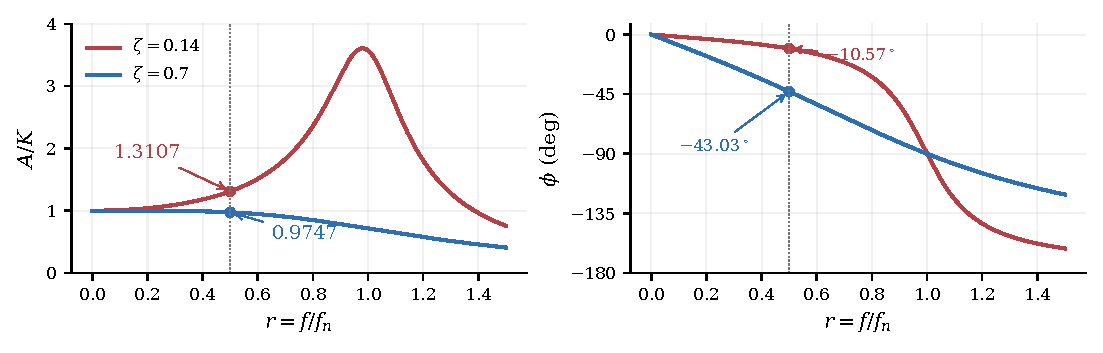
\includegraphics[width=.96\linewidth]{ch3-hw04-damping.pdf}
\end{center}
图中标出的 $r=0.5$ 即本题工作点。$\zeta=0.14$ 的共振峰在 $r_r\approx0.9802$，峰高约 $3.607$；$\zeta=0.7$ 的峰高仅约 $1.0002$。提高阻尼明显压低共振放大，并使本题工作点的幅值更接近静态标定值；相位滞后却由约 $10.57^\circ$ 增大到约 $43.03^\circ$。这说明适度阻尼改善幅值和瞬态振铃，同时需要接受并检查相位延迟。

\begin{focusbox}{知识主线}
把输入频率换成归一化工作点 $r=f/f_n$，由幅相响应评价该点的误差。静态标定、动态幅值校正和时延评价回答不同的问题；选择固有频率时应检查整个待测频带，不能只检查是否低于固有频率。
\end{focusbox}

\subsection*{本题知识点与公式}
\label{kn:3-4}
\noindent\textbf{已学前置：}第\ref{kn:3-3}节的二阶模型、频率比、幅相响应和阻尼折中，第\ref{kn:3-2}节的误差约束。
\textbf{本题新增：}工作点与动态灵敏度、静态标定后的动态误差、已知模型的单频校正、固有频率选取、相位延迟与群延迟。

\subsubsection*{1. 频率比如何把具体传感器放到通用曲线上}
二阶归一化特性只依赖 $r$ 和 $\zeta$，而非分别依赖输入频率与固有频率。因此同一阻尼下，把横轴写成 $r=f/f_n$，不同固有频率装置都可在同一条曲线上比较。这里 $f$ 与 $f_n$ 必须同用Hz，或 $\omega$ 与 $\omega_n$ 同用 $\mathrm{rad/s}$；不能一个用Hz、另一个用角频率。本题 $r=0.5$，表示输入角频率是无阻尼固有角频率的一半，不表示“输入已低到可以忽略所有动态误差”。

在此工作点，分母实部 $1-r^2=0.75$ 固定，虚部 $2\zeta r=\zeta$ 随阻尼变化。所以增大 $\zeta$ 会增大分母的模，使 $A$ 从 $1.310694$ 降到 $0.974740$；同时分母相角增大，使相位更滞后。由复平面上同一个分母即可解释幅值改善、相位滞后增大同时发生的原因。

\subsubsection*{2. 静态灵敏度、动态灵敏度与幅值校正}
设力传感器实际输出电压为 $U$，静态灵敏度为 $K_0>0$，单位 $\mathrm{V/N}$。若采用本题的二阶模型，其实际频率响应为
\[
H_{UF}(\iu\omega)=\frac{K_0}{1-r^2+\iu2\zeta r},\qquad
S_{\mathrm{dyn}}(\omega)=|H_{UF}(\iu\omega)|=K_0A(r).
\]
$S_{\mathrm{dyn}}$ 称该频率下的幅值动态灵敏度，单位仍是 $\mathrm{V/N}$；$A(r)$ 才是无量纲比值。静态标定把电压换为指示力 $z=U/K_0$，所以单频输入力幅值为 $F_0$ 时，指示幅值为 $Z_0=A(r)F_0$。有符号动态偏差为 $(A-1)\times100\%$，误差大小为 $|A-1|\times100\%$。

因此静态标定已知，并没有消除频率相关误差：本题两种阻尼分别仍会高估31.0694\%和低估2.5260\%。若频率和模型参数已准确获知，可按
\[
F_0=\frac{U_0}{K_0A(r)},\qquad
\theta_F=\theta_U-\phi(r)
\]
对单频的幅值与相位作动态校正，其中 $U_0,\theta_U$ 是所测输出电压的幅值和相位。复数形式就是 $\widehat F=\widehat U/H_{UF}(\iu\omega)$。多频信号必须逐频校正，不能用一个常数修正所有频率。

校正的适用前提是装置在线性范围内，$K_0,f_n,\zeta$ 及测量频率已知，而且该频率的输出具有足够信噪比。若输出中有噪声，其折算到输入的幅值会被 $1/|H_{UF}|$ 放大；当高频响应很小时，逆校正会明显放大噪声与模型误差。动态校正因而不能替代合理的传感器带宽与固有频率设计。

\subsubsection*{3. 如何按误差要求选择固有频率}
提高 $f_n$ 会减小给定 $f$ 的 $r$，使工作点靠近 $A(0)=1$、$\phi(0)=0$。但需要多高的 $f_n$，应由误差限和阻尼共同决定，不能仅要求 $f_n>f$。

设待测最高频率为 $f_m$，允许归一化幅值误差为 $0<\varepsilon<1$。从 $|A(r)-1|\leq\varepsilon$ 得
\[
1-\varepsilon\leq A(r)\leq1+\varepsilon.
\]
用第\ref{kn:3-3}节的 $D(r)=A^{-2}(r)$ 代入，等价于
\[
\boxed{\frac{1}{(1+\varepsilon)^2}
\leq1+(4\zeta^2-2)r^2+r^4
\leq\frac{1}{(1-\varepsilon)^2}}.
\]
给定 $\zeta$ 后，这是一组关于 $r$ 的不等式；令 $u=r^2\geq0$，即可化为二次不等式求解。应选出\textbf{从直流 $r=0$ 连续延伸且全段满足要求}的工作区间 $[0,r_A]$，再要求 $f_m/f_n\leq r_A$。低阻尼幅值先升后降，某个较高频率处偶然再次接近1，并不能证明此前整个频带都满足精度。

若还要求 $|\phi|\leq\phi_{\max}<\pi/2$，工作点必须位于 $r<1$。由
$2\zeta r/(1-r^2)\leq\tan\phi_{\max}$，整理二次不等式可得
\[
r\leq r_\phi
=\frac{\sqrt{\zeta^2+\tan^2\phi_{\max}}-\zeta}
{\tan\phi_{\max}},\qquad \phi_{\max}>0.
\]
所以覆盖从直流到 $f_m$ 的设计条件为
\[
\boxed{f_n\geq\frac{f_m}{\min(r_A,r_\phi)}}.
\]
这里的误差限是一般设计符号，原题并未指定，故无需为本题另造数值要求。原题给定 $f_n=800\,\mathrm{Hz}$ 后，直接在 $r=0.5$ 处检查即可；两种阻尼的误差比较已说明它们不能仅凭相同的固有频率视作等效装置。

\subsubsection*{4. 相位差换算的延迟与群延迟不是同一量}
对某个单频输入，若输出滞后 $\phi(\omega)$，可把它写成 $\omega(t-t_\phi)$，定义相位延迟
\[
\boxed{t_\phi(\omega)=-\frac{\phi(\omega)}{\omega}}.
\]
相位须用弧度，结果才是秒；应使用从低频连续展开的相位支。单频的周期性使延迟还存在整周期的不确定性，连续支约定用于在频率之间一致比较。本题输入角频率为 $800\pi\,\mathrm{rad/s}$，两种阻尼的相位延迟约为 $0.07343$ 与 $0.29879\,\mathrm{ms}$。该数值只表示此单频分量的相移，不能直接当作任何波形的整体传播时间。

若信号由某中心角频率 $\omega_c$ 附近的一小段频带组成，可在该处展开相位：
\[
\phi(\omega)\approx\phi(\omega_c)
+\left.\frac{\diff\phi}{\diff\omega}\right|_{\omega_c}(\omega-\omega_c).
\]
当该小频带内幅值近似不变、相位可近似成这条直线时，缓变包络经历的延迟由相位曲线的斜率决定，定义为\textbf{群延迟}
\[
\boxed{t_g(\omega)=-\frac{\diff\phi}{\diff\omega}}.
\]
相位延迟是相位与频率之比，群延迟是相位对频率的导数，单位均为秒。只有纯延迟 $\phi=-\omega t_d$ 时二者都等于同一个 $t_d$；频率相关相位一般不会使二者相等。

例如，一阶装置由第\ref{kn:3-1}节相位式直接得到
\[
t_\phi=\frac{\arctan(\omega\tau)}{\omega},\qquad
t_g=\frac{\tau}{1+(\omega\tau)^2}.
\]
二阶装置对 $\operatorname{atan2}(2\zeta r,1-r^2)$ 求导，分子为
$(1-r^2)2\zeta-(2\zeta r)(-2r)=2\zeta(1+r^2)$，再用 $\diff r/\diff\omega=1/\omega_n$，得到
\[
t_g(\omega)=\frac{2\zeta(1+r^2)}
{\omega_n\bigl[(1-r^2)^2+4\zeta^2r^2\bigr]}.
\]
在本题 $r=0.5$ 处，两种阻尼的群延迟约为 $0.11962$ 与 $0.33079\,\mathrm{ms}$，均与各自相位延迟不同。在 $r\to0$ 的极限下，两者才都趋向 $2\zeta/\omega_n$，与上一题的近似线性相位相符。理解这一差别，就能区分“某频率相位滞后较大”和“某个多频波形是否近似共同延迟”这两个判断。
\nt{\textbf{易错点：}本题 $r=0.5$ 并非共振点；“幅值比更接近1”不等于“相位滞后更小”。实际电压输出还需乘力传感器的静态灵敏度，题中未给出该值，不能为它指定数值。}

\chapter{传感原理和敏感元件}
\label{chap:hw-sensors}

\noindent 本章对应《课后作业-CH4》的全部7题。各题沿着“被测量改变什么物理量，测量电路怎样读出，哪些条件限制结论”展开；所列应用均用于解释原题，不另设练习。

\section{第1题：应变片电阻变化与电流表的可读性}
\label{sec:hw-sensors-1}
\label{hw:4-1}
\begin{hwquestion}
电阻应变片的灵敏度 $S_g=2$，初始电阻 $R=120\,\Omega$，工作应变为 $1000\,\mu\varepsilon$。求 $\Delta R$。将应变片与原图中的 $1.5\,\mathrm V$ 电源、电流表串联，求：（1）无应变时电流；（2）有应变时电流；（3）电流指示值的相对变化量；（4）分析该变化能否从表中读出。
\end{hwquestion}

\subsection*{答案与解析}
按正应变表示拉伸，忽略电源内阻、电流表内阻及导线电阻，供电电压恒为 $U=1.5\,\mathrm V$。先换算应变：
\[
\varepsilon=1000\times10^{-6}=10^{-3},\qquad
\frac{\Delta R}{R}=S_g\varepsilon=0.002.
\]
因此
\[
\boxed{\Delta R=RS_g\varepsilon=0.24\,\Omega},\qquad
R'=R+\Delta R=120.24\,\Omega.
\]
电流表的两个读数为
\[
\boxed{I_0=\frac{1.5}{120}=12.5\,\mathrm{mA}},\qquad
\boxed{I=\frac{1.5}{120.24}\approx12.47505\,\mathrm{mA}}.
\]
由此得到电流的绝对变化与相对变化：
\begin{align*}
\Delta I&=I-I_0\approx-0.02495\,\mathrm{mA}=-24.95\,\mu\mathrm A,\\
\boxed{\frac{\Delta I}{I_0}}
&=\frac{R}{R+\Delta R}-1
=-\frac{\Delta R/R}{1+\Delta R/R}
=\boxed{-0.001996\approx-0.1996\%}.
\end{align*}
正应变使电阻增大，恒压供电下电流减小。若只作一阶近似，则 $\Delta I/I_0\approx-\Delta R/R=-0.2\%$；精确结果的分母不能省略。

\textbf{能否读出：}原题未给电流表的量程、最小分度或数字分辨力，也未给噪声和漂移，因而不能作唯一判断。要可靠区分两个读数，表计应能分辨约 $25\,\mu\mathrm A$ 的变化，且重复读数的噪声、供电变化和温漂须足够小。该变化仅约占初始读数的 $0.2\%$，普通粗分度毫安表通常难以清楚辨别；合适的精密表计则可能读出。若使用准确度按满量程给出的模拟表，还需结合所选量程评估读数可信程度。

\subsection*{本题知识点与公式}\label{kn:4-1}
\noindent\textbf{本题新增：}建立“构件变形 $\to$ 敏感栅应变 $\to$ 电阻变化 $\to$ 电流或桥压”的完整关系。本题先讲应变计本体，完整单臂、半桥和全桥接线在信号调理部分继续展开。

\subsubsection*{1. 应变、电阻与灵敏度系数从何而来}
轴向工程应变定义为 $\varepsilon=\Delta l/l_0$，其中 $l_0$ 是未变形长度，$\Delta l$ 是沿所选方向的长度增量。应变无量纲，通常拉伸为正、压缩为负；$1\,\mu\varepsilon=10^{-6}$。它与应力不同：应力单位为Pa，单轴、小变形、线弹性条件下才有 $\sigma_m=E\varepsilon$，其中 $E$ 是杨氏模量。

均匀导体电阻满足
\[
R=\rho\frac{l}{A_s},\qquad
\frac{\diff R}{R}=\frac{\diff\rho}{\rho}
+\frac{\diff l}{l}-\frac{\diff A_s}{A_s}.
\]
$\rho$ 为电阻率（$\Omega\,\mathrm m$），$A_s$ 为敏感栅截面积（$\mathrm m^2$）。式中三个来源分别是材料电阻率改变、长度改变及截面积改变，不能只保留长度项。若敏感栅近似承受单轴应变，泊松比 $\nu=-\varepsilon_{\perp}/\varepsilon$，两横向尺寸相对应变均为 $-\nu\varepsilon$，则一阶近似有
\[
\frac{\Delta A_s}{A_s}\approx-2\nu\varepsilon,
\quad
\frac{\Delta R}{R}\approx(1+2\nu)\varepsilon+\frac{\Delta\rho}{\rho}.
\]
于是应变片灵敏度系数为
\[
\boxed{S_g=\frac{\Delta R/R}{\varepsilon}
\approx1+2\nu+\frac{\Delta\rho/\rho}{\varepsilon}},
\qquad \Delta R\approx RS_g\varepsilon.
\]
这里以小变化比值代表局部导数；$S_g$ 无量纲，应采用制造商标定值或题给值。\textbf{金属应变片}中几何变化很重要，电阻率变化也可能贡献，常见 $S_g$ 约为2；\textbf{半导体应变片}的压阻效应使电阻率随应力明显改变，通常灵敏度更大，但温度影响、非线性与个体差异也更显著。故不能把所有材料的 $S_g$ 都固定成 $1+2\nu$。

\subsubsection*{2. 应变片测的是哪个方向的应变}
粘贴式应变片依靠基底和胶层把构件表面变形传到敏感栅，主要测量栅轴方向的平均应变。栅线需与所求应变方向一致，粘贴不良、胶层蠕变和局部应变梯度都会改变读数。若表面平面应变分量为 $\varepsilon_x,\varepsilon_y,\gamma_{xy}$，栅轴相对 $x$ 方向夹角为 $\theta$，则
\[
\varepsilon_\theta=\varepsilon_x\cos^2\theta+
\varepsilon_y\sin^2\theta+\gamma_{xy}\sin\theta\cos\theta.
\]
$\gamma_{xy}$ 是工程剪应变，等于张量剪应变的两倍；角度误差不一定只造成一个余弦系数。未知主应变方向时，可用多个方向的应变片组成应变花，再由各方向读数重建应变状态。原题默认给定的 $1000\,\mu\varepsilon$ 就是栅轴方向的有效应变。

\subsubsection*{3. 温度交叉影响与激励自热}
温度既能改变敏感栅电阻率，也会引起栅、基底和构件的热膨胀不匹配。把这些影响在工作点附近合并为有效温度系数 $\alpha_{\mathrm{eff}}$（$\mathrm K^{-1}$），可写
\[
\frac{\Delta R}{R}\approx S_g\varepsilon+
\alpha_{\mathrm{eff}}\Delta T,\qquad
\varepsilon_{\mathrm{app}}=\frac{\alpha_{\mathrm{eff}}\Delta T}{S_g}.
\]
第二项会被误读为表观应变；$\alpha_{\mathrm{eff}}$ 随材料和安装条件而定，并非单一材料电阻温度系数的通用替代。温度还会改变 $S_g$，因此零点补偿和灵敏度温度补偿是两个问题。可采用匹配材料的自温度补偿片、同温补偿片和合理桥路减轻影响，仍须按实际温度范围标定。

电阻上的激励功率为 $P_g=I_g^2R=U_g^2/R$。提高激励会增大可测信号，同时增加自热；温升又反过来引起电阻漂移。应检查应变片允许功率、栅面积和构件散热条件，不能只为提高输出无限增大供电。\footnote{应变、桥路与温度补偿的器件说明可参见\href{https://www.ni.com/en/shop/data-acquisition/sensor-fundamentals/measuring-strain-with-strain-gages.html}{NI：Measuring Strain with Strain Gages}。}

\subsubsection*{4. 从电阻变化到可辨读数}
若串联回路还有固定电阻 $R_s$，则
\[
I(\varepsilon)=\frac{U}{R(1+S_g\varepsilon)+R_s},\quad
I_0=\frac{U}{R+R_s},\quad
\frac{\Delta I}{I_0}=-\frac{RS_g\varepsilon}{R+R_s+RS_g\varepsilon}.
\]
在零应变附近，电流对应变的局部灵敏度为
\[
S_{I\varepsilon}=\left.\frac{\diff I}{\diff\varepsilon}\right|_0
=-\frac{URS_g}{(R+R_s)^2},\qquad
\Delta\varepsilon_{\min}\approx\frac{\Delta I_{\min}}{|S_{I\varepsilon}|}.
\]
$S_{I\varepsilon}$ 的单位为A/应变，$\Delta I_{\min}$ 是电流输出端可辨变化；折算成微应变时应乘 $10^6$。由此可见，表内阻和引线电阻不仅改变基值，也会降低相对应变的读出能力。原题还缺少 $\Delta I_{\min}$、噪声及漂移，因此不能仅由理论 $\Delta I$ 断言仪表一定可读。

平衡电桥用两个分压点相减，把未受力时的大基值抵消，使微小变化便于差分放大。等臂、单臂变化、输出近似开路时，有
\[
|U_o|\approx\frac{U_e}{4}\left|\frac{\Delta R}{R}\right|
=\frac{U_eS_g}{4}|\varepsilon|.
\]
它说明电桥为何适合本题的微小电阻变化；准确系数、符号及半桥、全桥增敏条件须由具体接线推导，不能只按应变片数量判断。
\nt{\textbf{易错点：}$1000\,\mu\varepsilon=0.001$，不是 $0.001\%$；相对电阻变化为 $+0.2\%$，电流相对变化约为 $-0.1996\%$。分辨力说明能否区分变化，准确度还涉及偏差等因素，两者不能混用。}

\needspace{11\baselineskip}
\section{第2题：电容、电感和电阻应变式测量电路的异同}
\label{hw:4-2}
\begin{hwquestion}
电容式、电感式、电阻应变式传感器的测量电路有何异同？举例说明。
\end{hwquestion}

\subsection*{答案与解析}
\textbf{共同点：}三者都可先把被测量转换为电参数变化，即 $\Delta C$、$\Delta L$ 或 $\Delta R$，再借助外部激励和转换电路得到可测电压、电流或频率。测量链通常包含激励、参数转换、放大、必要的解调及滤波；差动结构、电桥和比值读出均可用于抑制部分共同干扰。

\begin{center}
\small
\begin{tabularx}{\linewidth}{@{}p{1.6cm} X X@{}}
\toprule
类型 & 典型读出电路与例子 & 主要区别和误差来源 \\
\midrule
电阻应变式 & 直流或交流电阻桥。应变使 $\Delta R/R=S_g\varepsilon$，桥路把电阻比变化变成差分电压。 & 可直接用直流激励；须注意导线电阻、供电稳定性、自热和温度补偿。 \\
电容式 & 交流电桥、交流阻抗分压、充放电计时或振荡调频。变极距位移使 $C=\varepsilon_0\varepsilon_r A/d$ 改变。 & $Z_C=1/(\iu\omega_e C)$；电容量常较小，对寄生电容、漏电、屏蔽和前端输入阻抗敏感。 \\
电感式 & 交流电桥、阻抗分压、差动变压器或振荡调频。气隙变化引起 $L$ 改变；差动变压器读二次差动电压。 & 线圈一般含 $R_w+\iu\omega_e L$，需考虑绕组电阻、磁滞、漏磁、损耗及外磁场；相位信息常有意义。 \\
\bottomrule
\end{tabularx}
\end{center}

直流电阻桥在理想条件下的平衡关系只涉及电阻比例；交流桥的平衡关系涉及\textbf{复阻抗比例}，通常须同时满足幅值与相位条件。对电容或电感施加恒定直流并等待暂态消失，不能仅由理想元件的稳态电压、电流读出其参数；因此常用交流或充放电等时变过程测量。

\subsection*{本题知识点与公式}\label{kn:4-2}
\noindent\textbf{已学前置：}\hyperref[kn:4-1]{第1题}已建立电阻应变转换与外部激励读出。本题新增电容、自感、互感的结构关系，以及三类参数共有的交流桥、时间和频率读出。频率响应的幅相概念见\hyperref[kn:3-1]{测试系统第1题知识点}。

\subsubsection*{1. 电容式：面积、极距和介质三种结构}
忽略边缘效应的平行板电容为
\[
C=\frac{\varepsilon_0\varepsilon_rA}{d},\qquad
\frac{\diff C}{C}=\frac{\diff\varepsilon_r}{\varepsilon_r}
+\frac{\diff A}{A}-\frac{\diff d}{d}.
\]
$C$ 的单位是F，$\varepsilon_0$ 为真空介电常数（F/m），$\varepsilon_r$ 为无量纲相对介电常数，$A$ 为有效重叠面积，$d$ 为极距。\textbf{变极距型}用膜片或动极板改变 $d$，局部灵敏度 $\diff C/\diff d=-\varepsilon_0\varepsilon_rA/d^2$；极距越小越灵敏，但允许行程、机械平行度、击穿和碰撞风险也更严格。若 $x>0$ 表示极距缩小，
\[
C(x)=\frac{C_0}{1-x/d_0},\qquad
\frac{\Delta C}{C_0}=\frac{x/d_0}{1-x/d_0}\approx\frac{x}{d_0}
\quad(|x|\ll d_0).
\]
\textbf{变面积型}保持极距不变，矩形极板重叠面积 $A=bx$ 时，$C=\varepsilon_0\varepsilon_r bx/d$，理想灵敏度为常数 $\varepsilon_0\varepsilon_r b/d$，适合较大位移或角位移。\textbf{变介质型}使介电常数或介质占据比例改变；例如介质沿极板长度方向插入、不同区域相当于并联时，
\[
C(x)=\frac{\varepsilon_0 b}{d}
\bigl[\varepsilon_r x+(l-x)\bigr].
\]
这里 $l$ 为极板总长，外部区域取空气；若介质沿电场方向分层，应按串联电容处理，不能直接沿用此式。液位、厚度和湿度测量都需明确几何与介质分布。

\textbf{差动结构的推导：}两侧间隙为 $d_0-x$、$d_0+x$，令 $r=x/d_0$，则
\[
C_1=\frac{C_0}{1-r},\quad C_2=\frac{C_0}{1+r},\quad
\frac{C_1-C_2}{C_0}=\frac{2r}{1-r^2},\quad
\boxed{\frac{C_1-C_2}{C_1+C_2}=r}.
\]
差值在零点附近灵敏度加倍并消除偶次项；\textbf{差值本身仍非严格线性，理想差和比才严格线性}。极板不平行、寄生电容和边缘效应会破坏理想关系。电容量小时，引线电容可能与信号同量级，需短引线、屏蔽、保护环或就近前置读出。

\subsubsection*{2. 自感、互感与涡流并非同一种转换链}
磁路近似中，磁动势 $NI=\mathcal R_m\Phi$，磁链 $\lambda_m=N\Phi$，由 $L=\lambda_m/I$ 得
\[
\boxed{L\approx\frac{N^2}{\mathcal R_m}},\qquad
\mathcal R_m=\sum_i\frac{l_i}{\mu_iA_i}.
\]
$N$ 为线圈匝数，$I$ 为电流（A），$\Phi$ 为磁通（Wb），$\lambda_m=N\Phi$ 为磁链；$L$ 的单位为H，$\mathcal R_m$ 为磁阻（A/Wb），$l_i,A_i$ 为第 $i$ 段磁路长度与截面积，$\mu_i$ 为磁导率（H/m）。若铁芯磁阻可忽略，总气隙长度为 $g$，则 $L\approx N^2\mu_0A/g$，有 $\diff L/\diff g=-L/g$。可变气隙式用位移改变磁阻；公式要求磁通近似均匀、漏磁和边缘效应较小且磁芯未饱和。

互感型通过一次线圈激励在二次线圈产生感应电压。差动变压器（LVDT）含两个反向串联的二次线圈，铁芯居中时互感近似相等。用一次电流相量 $I_p$ 表示，
\[
U_d=\iu\omega_e(M_1-M_2)I_p.
\]
在中心附近设 $M_1=M_0+k_Mx$、$M_2=M_0-k_Mx$，则 $U_d\approx\iu2\omega_e k_MI_px$。所以幅值反映位移大小，跨过零点时符号改变，等效载波相位翻转 $180^\circ$。实际若采用电压激励，一次电流还受一次阻抗影响；常用标定后的 $U_d\approx K_xxU_e$ 描述，不能把 $K_x$ 当成与激励频率无关的常数。\footnote{LVDT的耦合与同步解调见\href{https://www.analog.com/en/resources/reference-designs/circuits-from-the-lab/cn0371.html}{Analog Devices：CN0371}。}

涡流式则由交流磁场在导体中激发涡流，反作用使线圈的\textbf{等效电阻和电感同时变化}，读出量是 $Z=R_{\mathrm{eq}}+\iu\omega_eL_{\mathrm{eq}}$。间距、导电率、磁导率和缺陷都可能改变 $Z$；材料与检测深度问题在\hyperref[kn:4-5]{第5题}详细展开。

\subsubsection*{3. 从参数到时间、频率或桥压}
三种基本阻抗为 $Z_R=R$、$Z_C=1/(\iu\omega_e C)$、$Z_L=\iu\omega_e L$；实际电容有漏电和介质损耗，线圈有绕组电阻。\textbf{RC计时}利用 $U_C(t)=U_e(1-e^{-t/RC})$：达到固定阈值 $U_{\mathrm{th}}$ 所需时间为
\[
t_{\mathrm{th}}=-RC\ln\!\left(1-\frac{U_{\mathrm{th}}}{U_e}\right).
\]
在 $R$ 和阈值比固定时，$t_{\mathrm{th}}\propto C$；它可读静态电容，并不需要被测对象持续运动。\textbf{LC调频}利用 $f_r=(2\pi\sqrt{LC})^{-1}$，对数微分得到
\[
\frac{\Delta f_r}{f_r}\approx-\frac12
\left(\frac{\Delta L}{L}+\frac{\Delta C}{C}\right).
\]
固定一项即可读另一项；寄生参数、损耗和振荡器稳定性也会影响频率。

\textbf{交流桥的一般平衡：}规定左支路上、下臂为 $Z_1,Z_2$，右支路上、下臂为 $Z_3,Z_4$，桥源加在上下端，输出取左中点减右中点。输出开路时，
\[
U_o=U_e\left(\frac{Z_2}{Z_1+Z_2}-\frac{Z_4}{Z_3+Z_4}\right),\qquad
\boxed{Z_1Z_4=Z_2Z_3\ \Longleftrightarrow\ U_o=0}.
\]
交流平衡不仅要求阻抗模的比例匹配，还要求相角差匹配；纯电阻桥是其特例。若信号为 $u_s=A(x)\cos(\omega_et+\phi)$，与同频参考 $\cos\omega_et$ 相乘再低通，保留 $A(x)\cos\phi/2$。相敏读出因此能保留载波正反相对应的位移符号；单纯取绝对幅值会丢失方向。实际需先校准载波相差，且解调低通应通过被测变化、抑制高频乘积项。
\nt{\textbf{易错点：}“需要交流激励”不等于“只能测动态量”。静态位移也可使电容或电感保持在新值，再由持续交流激励读出。被测量变化频率与激励载波频率应分别标明。}

\needspace{11\baselineskip}
\section{第3题：光电传感器的类型、特点与被测量}
\label{hw:4-3}
\begin{hwquestion}
光电传感器包含哪几种类型？各有何特点？用光电式传感器可以测量哪些物理量？
\end{hwquestion}

\subsection*{答案与解析}
若按\textbf{光电转换的物理效应}分类，可分为以下三类；后两类均属于内光电效应。
\begin{enumerate}
\item \textbf{外光电效应型：}光子使电子逸出材料表面，由阳极收集形成电流。典型元件为光电管、光电倍增管；倍增管通过二次电子发射获得较高增益，适合弱光检测，但通常需高压供电，并应注意强光、背景光和噪声。
\item \textbf{光导效应型：}光照在材料内部产生或释放载流子，改变电导率。典型元件为光敏电阻，通常光照增强时电阻降低，需要外加电源读出；结构简单，但响应速度、线性、暗电阻与温度影响取决于材料。
\item \textbf{光生伏特效应型：}光生电子、空穴被结区内建电场分离，形成光电流或光电压。典型元件为光电池和以光伏模式工作的光电二极管；可在零外加偏压下检测光，但输出仍需合适电路读出。
\end{enumerate}
光电二极管也可反向偏置运行以改善速度等性能，此时常称光导模式；不能因此把它的工作过程等同于光敏电阻的电阻变化。

若按\textbf{光路布置}分类，又可说对射式、反射式、遮光式等；若按信息编码方式分类，可说模拟光强测量、脉冲计数、成像等。它们与上述物理效应分类处于不同层面，可相互组合。

\begin{center}
\small
\begin{tabularx}{\linewidth}{@{}p{2.8cm} X@{}}
\toprule
可测物理量 & 被测量到光电信号的转换关系 \\
\midrule
光强、光功率、照度 & 直接检测入射光；须匹配光谱响应并进行相应标定。 \\
位移、尺寸、振动 & 位移改变遮挡面积、反射光耦合或光斑位置，产生连续电信号。 \\
转速、角位移、计数 & 光栅或码盘周期遮光，把运动变为脉冲频率、相位或脉冲数。 \\
温度 & 目标热辐射的光强或光谱随温度变化，结合辐射模型与发射率求温度。 \\
浓度、液位、浑浊度 & 被测介质改变吸收、透射或散射，使接收光强或光谱变化。 \\
表面状态与缺陷 & 合适照明下，裂纹、划痕等改变反射、散射或图像对比度。 \\
\bottomrule
\end{tabularx}
\end{center}

\subsection*{本题知识点与公式}\label{kn:4-3}
\noindent\textbf{已学前置：}前两题说明用电参数变化读被测量。本题新增光到电的能量与载流子转换、光谱匹配，以及光学运动量的编码读出；傅里叶与频率概念沿用前章，不另作推导。

\subsubsection*{1. 三种光电效应的物理判别}
光子能量 $E_\gamma=h f_\gamma=hc/\lambda$，其中 $h$ 为普朗克常量（J$\cdot$s），$c$ 为真空光速，$\lambda$ 为真空波长。\textbf{外光电效应}要求光子提供足够能量使电子越过表面逸出势垒；理想阈值 $hf_\gamma\ge W$，最大初动能满足 $E_{k,\max}=hf_\gamma-W$。光电管用阳极收集逸出电子，光电倍增管再通过多个倍增极进行二次发射。倍增提高电流增益，也会带来暗计数、增益波动和强光过载，故“高增益”并不等同于无限低噪声。

\textbf{光导效应}不要求电子逸出材料。光照改变内部载流子浓度，使
\[
\sigma_e=q_e(n\mu_n+p\mu_p),\qquad
R=\frac{l}{\sigma_e A_s}
\]
发生变化。$q_e$ 为元电荷的正值，$n,p$ 为电子、空穴浓度（$\mathrm m^{-3}$），$\mu_n,\mu_p$ 为迁移率（$\mathrm m^2/(\mathrm{V\,s})$）。光敏电阻需要外部电源把电导变化变成电流或电压；载流子寿命长可能提高光导增益，同时使关光后的恢复变慢，因此灵敏度与速度常有取舍。

\textbf{光生伏特效应}用结区内建电场分离光生电子和空穴；短路时表现为光电流，开路时形成光电压。光电二极管可采用零偏光伏模式以减轻某些暗电流影响，也可反偏以减小结电容、改善速度；反偏需同时考虑暗电流和噪声。不能仅由“需要电源”与否给所有光电器件作统一性能排序。

对普通带间吸收半导体探测器，理想长波截止近似为 $\lambda_c=hc/E_g$，$E_g$ 是带隙能量；这说明波长太长时光子能量不足。实际还受吸收系数、表面窗口和材料结构影响，短波响应也有损失，应使用器件给定的光谱响应曲线，而非只用一个理论截止波长。

\subsubsection*{2. 响应度、量子效率和光电读出}
在给定波长的线性范围内，光电流满足 $I_{\mathrm{ph}}=\mathcal R_\lambda P_r$，$\mathcal R_\lambda$ 的单位为A/W。外量子效率定义为收集到的电子数率与入射光子数率之比：
\[
\eta_q=\frac{I_{\mathrm{ph}}/q_e}{P_r/(hc/\lambda)},\qquad
\boxed{\mathcal R_\lambda=\eta_q\frac{q_e\lambda}{hc}}.
\]
该式适用于无内部倍增、按所定义收集电子计数的情况；具有光导增益或雪崩倍增时应明确是否另计增益。由此可知，同一量子效率下A/W响应度也随波长变化。照度以lux计，光功率以W计，两者分别涉及人眼加权与辐射量，不能在没有光谱条件时直接互换。\footnote{光谱响应度、量子效率及噪声的器件解释见\href{https://hub.hamamatsu.com/us/en/technical-notes/detector-selection/guide-to-detector-selection.html}{Hamamatsu：Guide to detector selection}和\href{https://hub.hamamatsu.com/us/en/technical-notes/detector-selection/the-wits-guide-to-selecting-a-photodetector.html}{WITS detector guide}。}

光电流可由跨阻放大器转换为 $U_o\approx-R_fI_{\mathrm{ph}}$，但该关系要求放大器在线性工作频带内、输出不饱和，且反馈与输入电容得到适当处理。若被测量 $x$ 通过光路改变 $P_r$，则
\[
\frac{\diff U_o}{\diff x}\approx
-R_f\mathcal R_\lambda\frac{\diff P_r}{\diff x}.
\]
所以位移、浓度等的灵敏度由“光路斜率 $\times$ 光电响应度 $\times$ 电路增益”共同决定。反射率、污染、光源波动也会改变 $P_r$，可通过参考通道、比值读出或同步检测减轻干扰。

\subsubsection*{3. 从遮光脉冲到位移、方向和转速}
对射式由目标遮断光束，反射式由目标返回光；连续遮光面积或光斑位置变化可读模拟位移，周期光栅与码盘则把运动变成计数。设增量码盘每相每转有 $N$ 个完整周期，计数倍频因子 $q_c=1,2,4$，则
\[
N_{\mathrm{cnt}}=q_cN,\qquad
\Delta\theta=\frac{360^\circ}{q_cN},\qquad
\theta-\theta_0=m\Delta\theta.
\]
$m$ 是带方向的累计计数。A、B两路相差四分之一周期，哪一路超前随转动方向改变，故用正交相位顺序判向；四倍计数同时利用两路上、下沿。若 $f_{\mathrm{cnt}}$ 是按同一规则统计的每秒计数事件数，转速大小为
\[
n_{\mathrm{rot}}=\frac{60f_{\mathrm{cnt}}}{q_cN}\quad(\mathrm{r/min}).
\]
若使用单路周期频率 $f_A$，则应写 $60f_A/N$，不能再次除以4。增量式断电后通常需重新建立参考零位；绝对码盘用 $n_b$ 位编码标识位置，理想角分辨力为 $360^\circ/2^{n_b}$。格雷码使相邻位置只变一位，可减轻过渡区多位不同步引起的粗大误码，但分辨力仍不代表机械与光学准确度。

\subsubsection*{4. 弱光、强光与响应速度的使用边界}
\textbf{暗电流}是无入射光时仍存在的电流；背景光则是实际入射的非目标光，两者来源不同。二者以及光电流都会带来噪声。以散粒噪声模型说明，在等效噪声带宽 $B_n$ 内，若相关电流为 $I_d+I_{\mathrm{ph}}$，则
\[
i_{n,\mathrm{shot,rms}}\approx
\sqrt{2q_e(I_d+I_{\mathrm{ph}})B_n}.
\]
公式说明扩大读出带宽会增加所收集的白噪声；电阻热噪声和放大器噪声还需另计。缩窄带宽有助于弱光检测，却不能窄到削弱所需动态信号。噪声设定弱光下限，结区、倍增或放大器饱和设定强光上限；二者之间还需检查非线性。器件的响应时间、结电容及后级时间常数共同限制高速计数能力，应结合\hyperref[kn:3-2]{一阶系统的带宽与误差条件}评估漏计、脉冲展宽和相位滞后。
\nt{\textbf{易错点：}光电传感器最终可测多种物理量，但探测器直接接收的是光。温度测量还需发射率等条件，反射式位移测量还需目标表面和光路标定，不能把光强变化唯一归因于被测量。}

\needspace{11\baselineskip}
\section{第4题：霍尔效应的本质与三种应用}
\label{hw:4-4}
\begin{hwquestion}
何谓霍尔效应？其物理本质是什么？用霍尔元件可测哪些物理量？请举出三个例子说明。
\end{hwquestion}

\subsection*{答案与解析}
\textbf{霍尔效应：}通电导体或半导体置于与电流方向有垂直分量的磁场中，会在同时垂直于电流和磁场的方向产生横向电场及电势差，这一电势差称为霍尔电压。

\textbf{物理本质：}漂移载流子受洛伦兹力 $q\mathbf v_d\times\mathbf B$ 横向偏转，在侧边积累电荷。积累电荷产生霍尔电场，直至横向电场力与磁力平衡。单一载流子、均匀薄片的理想模型给出
\[
U_H=R_H\frac{I_bB_\perp}{d}=K_HI_bB_\perp,
\qquad R_H\approx\frac{1}{nq},\quad K_H=\frac{R_H}{d}.
\]
其中 $I_b$ 为偏置电流，$d$ 为薄片厚度，$B_\perp$ 为垂直片面的磁感应强度，$n$ 为载流子数密度。$R_H$ 的符号与载流子类型及约定有关，输出极性还受电流、磁场和引线方向影响。

\begin{enumerate}
\item \textbf{测磁场：}保持偏置电流恒定并扣除零偏，由 $B_\perp=U_H/(K_HI_b)$ 得到磁场分量。恒定磁场也可产生稳定霍尔电压。
\item \textbf{测电流：}被测导线电流 $I_m$ 产生磁场，霍尔元件检测该磁场。若磁路在线性范围内且已标定 $B_\perp=k_I I_m$，则 $U_H=K_HI_bk_I I_m$，可测直流或适当带宽内的交流电流。被测电流与霍尔片偏置电流是两个不同量。
\item \textbf{测转速：}转子上的磁体或齿轮磁路使磁场周期变化，经阈值处理得到脉冲。若每转输出 $N_p$ 个脉冲，脉冲频率为 $f_p$，则
\[
\boxed{n=\frac{60f_p}{N_p}\quad(\mathrm{r/min})}.
\]
也可由脉冲数测转动增量，具体角分辨力取决于磁极及编码结构。
\end{enumerate}
此外，借助已标定的磁体或磁路，把位移、液位等转换为 $B_\perp$ 的变化，也可间接测量这些量。

\subsection*{本题知识点与公式}\label{kn:4-4}
\noindent\textbf{已学前置：}\hyperref[kn:4-3]{第3题}已讲脉冲计数、方向与转速换算，本题不重复编码器公式；本题新增洛伦兹力与霍尔电压、磁场到其他被测量的转换，以及与磁电感应的区别。

\subsubsection*{1. 从横向受力平衡推到霍尔电压}
设电流沿薄片长方向 $x$ 流动，磁场沿片面法向 $z$，宽为 $w$，厚为 $d$。载流子漂移速度 $\mathbf v_d$、电荷为带符号的 $q$，其横向力平衡为
\[
q(\mathbf E_H+\mathbf v_d\times\mathbf B)=0,
\qquad \mathbf E_H=-\mathbf v_d\times\mathbf B.
\]
横向电场不是外电源直接施加，而是载流子偏转后积累电荷建立的。对单一载流子、均匀薄片，电流密度 $J_x=nqv_x$，故在所选坐标下有 $E_y=J_xB_z/(nq)$。定义霍尔系数 $R_H=E_y/(J_xB_z)$，并取相应电极极性，利用 $I_b=J_xwd$ 与霍尔电压的幅值 $|E_y|w$ 得
\[
\boxed{U_H=R_H\frac{I_bB_\perp}{d}=K_HI_bB_\perp},
\quad R_H\approx\frac{1}{nq},\quad K_H=R_H/d.
\]
宽度在推导中抵消，厚度越小、载流子浓度越低，理想电流相关灵敏度越大，但电阻、噪声、发热和工艺会限制实际选择。多类载流子、复杂能带和散射条件下，$R_H$ 不一定精确等于 $1/(nq)$，考试中的简单公式应附上单载流子模型条件。

各量单位应相容：$U_H$ 为V，$I_b$ 为A，$B$ 为T，$d$ 为m，$R_H$ 为$\mathrm m^3/\mathrm C$，$K_H$ 为$\mathrm{V/(A\,T)}$。注意 $B$ 是磁感应强度，不能把以A/m计的磁场强度 $H$ 直接代入；线性材料中还需 $B=\mu H$。
\footnote{洛伦兹力平衡与霍尔电压的薄片模型见\href{https://www.nist.gov/pml/nanoscale-device-characterization-division/popular-links/hall-effect/hall-effect}{NIST：The Hall Effect}。}

\subsubsection*{2. 电压方向、零偏与偏置条件}
电压是两电极的电势差，方向应根据载流子符号、$\mathbf v_d\times\mathbf B$ 和电极次序判断，不能只记“上正下负”。固定器件与接线后，单独反转 $I_b$ 或 $B_\perp$ 会使理想霍尔电压反号，同时反转二者则不变。换成相反类型的多数载流子时，$R_H$ 的符号也会变化。

实际端口可写 $U_{\mathrm{meas}}=K_H(T)I_bB_\perp+U_{\mathrm{off}}(T)$。零偏可能来自电极不对称、热电势及应力，温度还会改变灵敏度。应采用稳定偏置、零场扣偏和温度标定；减小厚度或提高偏置电流虽会提高信号，也可能使发热与噪声变大。公式中的 $I_b$ 始终是\textbf{流过霍尔片的控制电流}，与被测导线中的大电流 $I_m$ 不同。

\subsubsection*{3. 三类应用各需要什么中间关系}
\textbf{磁场测量}直接利用校准后的 $U_H\to B_\perp$。若片面法向与磁场夹角为 $\alpha$，$B_\perp=B\cos\alpha$，装配角度误差会改变读数。

\textbf{电流测量}先由被测电流产生磁场。对足够长、周围近似空气的直导线，在径向距离 $r$ 处有 $B=\mu_0I_m/(2\pi r)$；磁芯集中磁通结构则用标定关系 $B_\perp=k_I I_m$。霍尔电压再反推 $I_m$。磁芯饱和、气隙、导体位置和外部磁场会破坏理想比例，因此不能把直导线公式与任意闭合磁路混用。由于静态电流也能产生静磁场，该方案可测直流，这是其重要特点。

\textbf{运动测量}由磁体或齿轮使磁场随位置变化，连续标定 $B_\perp(x)$ 可测位移，周期阈值检测可测转速。局部位移灵敏度为
\[
\frac{\diff U_H}{\diff x}=K_HI_b\frac{\diff B_\perp}{\diff x}.
\]
磁场对位置常非线性，所以需选择单调区；单路脉冲只给周期或计数，若要判断方向，还须采用附加相位或位置通道，计数约定沿用\hyperref[kn:4-3]{第3题}。

\subsubsection*{4. 与磁电感应式的原理边界}
磁电感应线圈依据
\[
e=-N\frac{\diff\Phi}{\diff t},\qquad
\Phi=\int\mathbf B\cdot\diff\mathbf S.
\]
它直接响应磁通变化率，静止线圈处在恒定磁通中输出为零；若磁通来自变化位置，输出常与运动速度有关。霍尔式在稳定偏置下可响应静磁场，两种元件都可用于测速，却不能互换其传递关系。运动线圈理想情形的 $e=Blv$ 还要求导线、运动与磁场方向满足相应几何关系；它不是霍尔电压公式，也不意味着能直接读静态位移。
\nt{\textbf{易错点：}霍尔片直接敏感的是磁场，测电流、位移或转速须说明中间的磁场转换关系。由 $U_H\propto B$ 不能推出任意磁路中都有 $U_H\propto x$。}

\needspace{11\baselineskip}
\section{第5题：涡轮机叶片裂纹检测}
\label{hw:4-5}
\begin{hwquestion}
有一批涡轮机叶片，需要检测是否有裂纹，请举出两种以上方法，并阐明所用传感器的工作原理。
\end{hwquestion}

\subsection*{答案与解析}
原题未限定叶片材料、涂层及裂纹位置。可优先说明\textbf{涡流与超声}两种方法，再根据材料与缺陷条件选取补充方法。

\textbf{方法一：涡流检测。}交流线圈在导电叶片中激发涡流；裂纹使涡流路径中断或绕行，改变涡流的反作用磁场和损耗，从而改变探头线圈的等效阻抗。检测其幅值、相位变化并扫描，可发现异常。
\[
\text{裂纹}\longrightarrow\text{涡流分布改变}
\longrightarrow\Delta Z_{\mathrm{coil}}\longrightarrow\text{电信号}.
\]
此法适合\textbf{导电材料的表面和近表面裂纹}，不要求材料必须铁磁，但常规涡流法不能直接用于绝缘陶瓷。抬离、曲率、涂层、裂纹方向及材料电磁性质都会影响判读。

\textbf{方法二：压电超声检测。}探头受电脉冲激励，利用\textbf{逆压电效应}发射超声；声波遇到裂纹等声学界面产生反射，探头再用\textbf{正压电效应}把回波转换为电信号。脉冲反射法根据异常回波的幅度和时间判断缺陷。若声速为 $c_s$，声束沿已知直线路径往返传播，回波时间为 $\Delta t$，则相应路径深度为
\[
h=\frac{c_s\Delta t}{2}.
\]
此法可检测适合声束探测的内部或一定深度的缺陷，但须保证耦合、探头入射方向及几何条件合适。薄壁、复杂曲面、粗晶和近表面盲区会影响检测效果。

\begin{center}
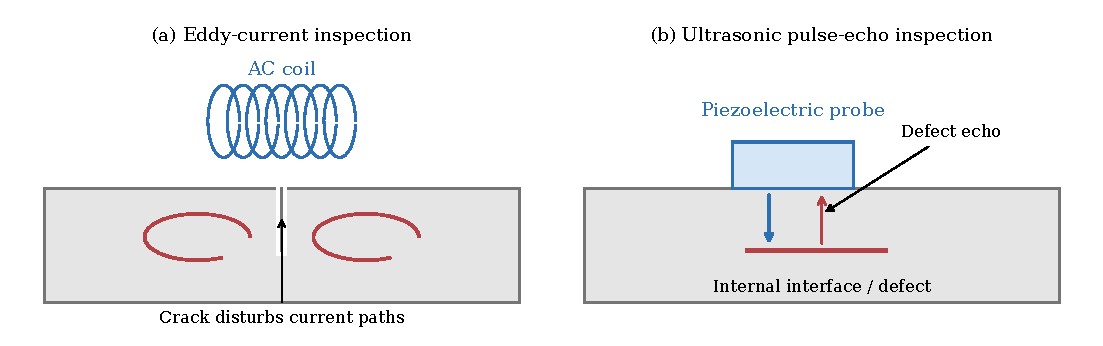
\includegraphics[width=.94\linewidth]{ch4-crack-detection.pdf}
\end{center}
\noindent 上图对比涡流受裂纹扰动和超声遇缺陷反射的机制；实际声束和扫描方向需依据叶片形状与预期裂纹取向设置。

\textbf{方法三：渗透显示配合光学检测。}对致密非多孔材料的\textbf{表面开口裂纹}，渗透液借毛细作用进入裂纹，去除表面多余渗透液后，经显像或荧光照明增强对比，再由相机等光电元件采集。它不能检出完全封闭在内部的裂纹，表面需清洁且开口不能被涂层遮挡。

\textbf{有条件的补充：磁性检测。}若叶片为\textbf{铁磁性材料}，磁化后裂纹附近会形成漏磁场，可由磁粉聚集显示，或由霍尔、磁阻等元件检测。该法不能因叶片“是金属”便直接采用，须先确认其磁性及磁化方向。

\subsection*{本题知识点与公式}\label{kn:4-5}
\noindent\textbf{已学前置：}\hyperref[kn:4-2]{第2题}已讲线圈、互感与涡流阻抗读出，\hyperref[kn:4-3]{第3题}已讲光电成像，\hyperref[kn:4-4]{第4题}已讲磁敏元件。本题新增无损检测的缺陷作用机制、趋肤深度和声学界面关系，重点是方法对材料、位置与取向是否成立。

\subsubsection*{1. 涡流为何改变探头阻抗}
涡流探头与导体可近似理解为一次线圈和一个分布式短路二次回路。用等效二次阻抗 $Z_s=R_s+\iu\omega_e L_s$、互感 $M$ 表示，二次感应电流为 $I_s=-\iu\omega_e MI_p/Z_s$，故一次端的反映阻抗为
\[
Z_{\mathrm{in}}=R_p+\iu\omega_e L_p+
\frac{\omega_e^2M^2}{R_s+\iu\omega_e L_s}.
\]
最后一项的实部代表附加损耗、虚部改变等效电感；这解释了为何实际检测通常同时分析阻抗幅值与相位。裂纹使局部电流绕行，改变等效耦合与阻抗，但抬离、边缘、曲率、涂层和材料变化也会改变这些量，因此异常信号需与参考试样及扫描位置对照。

\subsubsection*{2. 趋肤深度的来源、单位与频率选择}
均匀、线性、足够厚的良导体中，取时间因子 $e^{\iu\omega_et}$ 并忽略位移电流，麦克斯韦方程可化为一维磁场扩散方程
\[
\frac{\diff^2 H}{\diff z^2}=\iu\omega_e\mu\sigma_e H.
\]
沿深度 $z$ 衰减的解为
\[
H(z)=H(0)e^{-(1+\iu)z/\delta_s},\qquad
\boxed{\delta_s=\sqrt{\frac{2}{\omega_e\mu\sigma_e}}
=\sqrt{\frac{2\rho}{\omega_e\mu}}}.
\]
$\rho$ 是电阻率（$\Omega\,\mathrm m$），$\sigma_e=1/\rho$ 为电导率（S/m），$\mu$ 为绝对磁导率（H/m），$\omega_e=2\pi f_e$。把相对磁导率 $\mu_r$ 代入前须乘 $\mu_0$。$\delta_s$ 是场或电流密度幅值降至表面 $e^{-1}\approx36.8\%$ 的深度，既不是幅值降为零的位置，也不是通用的最大可检裂纹深度；相位还随深度滞后 $z/\delta_s$。

由 $\delta_s\propto f_e^{-1/2}\mu^{-1/2}\sigma_e^{-1/2}$ 可知，提高频率、磁导率或电导率都会减小标准穿透深度。高频有利于表层分辨，却更难深入；降低频率增加穿透，也可能降低细小表面缺陷的对比度。真实叶片的有限厚度、探头尺寸及弯曲表面不完全满足半空间模型，应把公式用于理解趋势与初选频率，再用试块验证。\footnote{趋肤深度及其幅值定义见\href{https://www.twi-global.com/technical-knowledge/faqs/faq-how-far-can-eddy-currents-penetrate}{TWI：How far can eddy currents penetrate?}；公式的均匀导体模型亦见\href{https://ansyshelp.ansys.com/public/views/secured/electronics/v242/en/subsystems/maxwell/content/SkinDepthforanEddyCurrentSolution.htm}{Ansys：Skin Depth for an Eddy Current Solution}。}

裂纹若大致平行于主涡流方向，阻断作用可能较弱；近似垂直于主电流路径时扰动更明显。故应改变扫描与励磁方向，而非只在某一位置读一次阻抗。涡流法要求导电，但并不要求铁磁；对铁磁材料，还需注意磁导率变化本身可能形成较强干扰。

\subsubsection*{3. 压电超声的发射、接收与缺陷回波}
压电材料的\textbf{正效应}把机械应力转为极化电荷，给定结构下可写 $Q=d_FF$，$d_F$ 单位为C/N；\textbf{逆效应}把电场转为机械应变，线性近似 $S=d_pE_e$，$d_p$ 单位为m/V，方向与晶体或陶瓷极化有关。探头发射利用逆效应，接收利用正效应；这两个过程组成“电信号 $\to$ 声波 $\to$ 缺陷反射 $\to$ 电信号”的完整链。

对均匀介质中的一维行波，特性声阻抗为
\[
Z_a=\rho_m c_s\quad
\bigl[\mathrm{kg/(m^2\,s)}\bigr],
\]
其中 $\rho_m$ 为质量密度，须与前面的电阻率 $\rho$ 区分。正常入射、平面界面、无损模型下，声压反射系数与强度反射率分别为
\[
r_p=\frac{Z_{a2}-Z_{a1}}{Z_{a2}+Z_{a1}},\qquad
\mathcal R_I=|r_p|^2.
\]
空气裂隙与金属的声阻抗差通常很大，能产生强反射；但探头与叶片之间若存在空气，也会阻碍声能进入工件，所以常需耦合剂或适当的非接触超声方案。式中 $r_p$ 可正可负，表示声压相位关系；$\mathcal R_I$ 是能量比，不能直接把两者相等。\footnote{声阻抗与界面反射的器件解释见\href{https://www.murata.com/products/sensor/ultrasonic/overview/basic/nature}{Murata：Properties of sound waves}；正常入射的反射关系可参见\href{https://hyperphysics.phy-astr.gsu.edu/hbase/Sound/acousimp.html}{Georgia State University：Acoustic Impedance}。}

在扣除仪器、耦合层及楔块延迟后，往返时间给出声程 $l=c_s\Delta t/2$。只有正入射且声程沿深度时才直接有 $h=l$；若声束在工件内与深度方向成角 $\theta$，则简单平面几何下 $h=l\cos\theta$。纵波、横波的声速不同，必须采用实际波型的材料声速。

探测能力还取决于波长 $\lambda_s=c_s/f_u$、脉冲长度、声束宽度与衰减。短脉冲有利于分开相邻回波，轴向分辨距离量级为 $c_s\tau_p/2$；提高频率通常改善小尺度分辨，却增加许多材料中的传播衰减。平面裂纹具有方向性，若镜面反射不返回接收探头，裂纹存在也可能回波弱，应采用多角度或阵列扫描。超声可用于适当声学条件下的金属、陶瓷等，不以导电或铁磁性为必要条件，但粗晶、薄壁和复杂曲面可能明显限制效果。

\subsubsection*{4. 磁性与渗透法各补充哪类缺陷}
磁粉与漏磁检测先磁化\textbf{铁磁性}工件。裂纹使磁路磁阻增大，局部磁通逸出表面；磁粉在漏磁场附近聚集，或由\hyperref[kn:4-4]{霍尔等磁敏元件}检测。缺陷对磁通的阻断程度随方向而变，必要时用两个励磁方向；非铁磁金属不能因为“导电”就直接采用磁粉法。

渗透法依靠润湿和毛细作用把液体带入\textbf{表面开口}裂纹，清除表面多余渗透液后显像，再作可见光或荧光观察。它对导电性、磁性没有上述要求，适用于合适的致密非多孔材料；封闭内部裂纹、被涂层堵住的开口和多孔表面都不宜直接套用。\footnote{原理及适用边界见\href{https://www-pub.iaea.org/MTCD/Publications/PDF/TCS-11.pdf}{IAEA：Liquid Penetrant and Magnetic Particle Testing}。}
因此本题若只要求“是否存在裂纹”，也应先规定材料和缺陷范围，再用相应参考缺陷建立判据；检测、定位和定量尺寸评估是不同层次的结论。
\nt{\textbf{易错点：}涡流需导电，磁性方法还需材料具有适用的磁性；两者不能混为一谈。超声发射用逆压电效应，接收用正压电效应，传播速度应取叶片材料内相应波型的声速。发现异常不等于已定量测出裂纹深度。}

\Needspace{11\baselineskip}
\section{第6题：光纤测压力与位移的工作原理}
\label{hw:4-6}
\begin{hwquestion}
说明用光纤传感器测量压力和位移的工作原理，指出其不同点。
\end{hwquestion}

\subsection*{答案与解析}
光纤可传输光，也可作为敏感元件。被测量改变光的强度、相位、偏振或波长，再由光电器件及解调电路读出。以\textbf{反射强度式光纤结构}说明两种测量，可直接比较其共同点与不同点。

\textbf{测位移：}发射光纤把光照向随被测对象移动的反射面，接收光纤收集反射光。间距 $d$ 改变时，光斑和接收耦合效率 $\eta(d)$ 改变，接收功率为
\[
P_r=P_t\eta(d),\qquad d=d_0+x.
\]
光电读出经标定后可将输出换为位移 $x$。应在 $\eta(d)$ 的合适单调区工作，避免同一输出对应两个间距。

\textbf{测压力：}把反射面制成受压弹性膜片。压力差 $p$ 使膜片产生位移 $x_d$，再改变光纤端面与膜片间距，从而改变接收光强。局部线性范围内可写
\[
p\longrightarrow x_d=k_pp
\longrightarrow d=d_0-x_d
\longrightarrow P_r=P_t\eta(d)\longrightarrow U_o.
\]
若光电及电路增益为 $G$，即 $U_o=GP_r$，则局部压力灵敏度为
\[
\frac{\diff U_o}{\diff p}=-GP_t\eta'(d)k_p.
\]
该式同时反映膜片机械灵敏度、光学耦合斜率和电路增益；输出正负取决于间距定义与工作分支。

\begin{center}
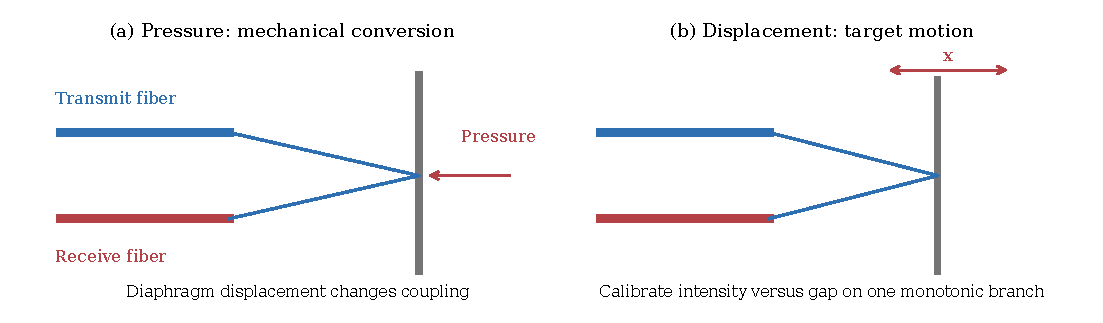
\includegraphics[width=.94\linewidth]{ch4-fiber-pressure-displacement.pdf}
\end{center}

\begin{center}
\small
\begin{tabularx}{\linewidth}{@{}p{2.1cm} X X@{}}
\toprule
比较项 & 位移测量 & 压力测量 \\
\midrule
机械输入 & 目标位移直接改变光学间距。 & 压力先使膜片等弹性体变形，再改变光学间距或应变。 \\
共同读出 & \multicolumn{2}{p{11.5cm}@{}}{均可采用强度、相位或波长调制；上述示例均用反射强度调制和光电转换。} \\
主要标定 & 光路、反射率、间距与输出关系及单调工作区。 & 除光学读出外，还需标定膜片刚度、温度及压力差边界条件。 \\
动态限制 & 目标运动与光电读出带宽。 & 还受膜片固有频率、阻尼及压力传递过程限制。 \\
\bottomrule
\end{tabularx}
\end{center}

\subsection*{本题知识点与公式}\label{kn:4-6}
\noindent\textbf{已学前置：}光到电的响应度和读出见\hyperref[kn:4-3]{第3题}，机械应变见\hyperref[kn:4-1]{第1题}，机械幅相响应见\hyperref[kn:3-3]{二阶系统知识点}。本题新增导光条件、三类光学调制和压力到光学量的弹性转换，重点解释压力与位移测量为何可共用同一光学读出。

\subsubsection*{1. 光纤如何导光，为什么间距会改变接收光}
普通阶跃型光纤由折射率较高的纤芯 $n_1$ 和较低的包层 $n_2$ 构成，$n_1>n_2$。在几何光学的子午光线近似下，纤芯到包层的入射角相对法线大于临界角
\[
\theta_c=\arcsin(n_2/n_1)
\]
时发生全反射。若外部介质折射率为 $n_0$，入射光相对纤轴的最大接收半角为 $\theta_a$，由端面折射和全反射条件可得数值孔径
\[
\boxed{\mathrm{NA}=n_0\sin\theta_a=\sqrt{n_1^2-n_2^2}}.
\]
数值孔径无量纲，描述可接收光锥的范围；不是越大测量就必然越准。上述光线公式适用于相应阶跃型导光模型，单模光纤的场分布和耦合还需波动光学描述。\footnote{全反射和接收角关系见\href{https://bop-iitk.vlabs.ac.in/exp/numerical-aperture-measurement/theory.html}{IIT Kanpur Virtual Labs：Numerical aperture measurement}。}

反射强度式探头的发射光形成扩展光斑，反射后只有落入接收纤端面且角度满足耦合条件的部分进入光纤，所以 $P_r=P_t\eta(d)$ 随间距改变。这里 $\eta$ 是包括光路几何与反射损失的耦合效率，不是第3题的量子效率 $\eta_q$。$\eta(d)$ 往往有峰值和不同斜率分支，需选定单调区；小变化时 $\Delta P_r\approx P_t\eta'(d_0)\Delta d$，在峰值处 $\eta'\approx0$，反而不适合灵敏位移读出。参考光路或比值 $P_r/P_{\mathrm{ref}}$ 可减轻共同光源功率波动，但不能自动消除目标反射率、弯曲损耗与几何变化。

\subsubsection*{2. 压力多了一段弹性机械转换}
位移测量中，目标运动直接使间距变化。压力是单位面积上的法向载荷（Pa），反射膜片受到的通常是两侧\textbf{压力差} $p=p_{\mathrm{in}}-p_{\mathrm{out}}$，并非没有参考条件的绝对压力。

以半径 $a$、厚度 $t_m$、周边固支的均匀圆形薄膜片为明确模型。材料各向同性、线弹性，均匀压力下的小挠度板弯曲刚度为
\[
D_b=\frac{Et_m^3}{12(1-\nu^2)}.
\]
$D_b$ 单位为N$\cdot$m。薄板方程 $D_b\nabla^4w=p$ 配合边缘条件 $w(a)=0$、$w'(a)=0$，得到
\[
w(r)=\frac{p}{64D_b}(a^2-r^2)^2,
\qquad
\boxed{w_0=\frac{pa^4}{64D_b}
=\frac{3(1-\nu^2)pa^4}{16Et_m^3}}.
\]
这里 $w_0$ 为中心挠度，$E$ 的单位为Pa，$a,t_m,w_0$ 均用m；模型要求薄板、挠度相对厚度足够小、无显著初始张力及塑性，边界确为固支。大挠度时膜内拉力变得重要，不能继续把上式线性外推。其他膜片形状、波纹和支承方式的系数也不同。\footnote{固支圆板的边界条件与解见\href{https://pkel015.connect.amazon.auckland.ac.nz/SolidMechanicsBooks/Part_II/06_PlateTheory/06_PlateTheory_05_RectangularCoordinates.pdf}{P. Kelly：Solid Mechanics Part II，Section 6.5}。}

于是本题示例的 $k_p=w_0/p$ 单位为m/Pa。若间距 $d=d_0-w_0$、光电总增益 $G$ 的单位为V/W，便有
\[
\frac{\diff U_o}{\diff p}=
\underbrace{G}_{\text{电路与光电}}
\underbrace{P_t\eta'(d)}_{\text{光学耦合}}
\underbrace{(-k_p)}_{\text{压力到位移}},
\]
输出灵敏度单位为V/Pa。增大半径或减薄膜片会提高静态灵敏度，也会降低刚度并影响固有频率、过载与线性范围。把膜片的主模态近似为二阶系统时，其归一化幅相规律沿用\hyperref[kn:3-3]{测试系统的二阶模型}；测压系统还可能受到引压管、腔体及光电读出带宽限制。

\subsubsection*{3. 相位式：读光程，不只读光强大小}
两束相干光叠加时，探测强度可写
\[
I=I_1+I_2+2V_c\sqrt{I_1I_2}\cos\Delta\phi,
\quad 0\le V_c\le1.
\]
$V_c$ 是可见度相关因子，反映相干、偏振和空间重叠等条件。反射腔的往返相位含 $\Delta\phi=4\pi nd/\lambda+\phi_0$；当折射率 $n$ 固定时，$\Delta(\Delta\phi)=4\pi n\Delta d/\lambda$。单个强度读数对相位是周期且多值的，小位移常在正交工作点附近线性读出，大范围位移则需条纹计数或相位解缠；一整条纹对应间距变化 $\lambda/(2n)$。温度也能改变 $n$、腔长和参考光程，需稳定或补偿。

压力若通过膜片改变同一腔长，也能用上述相位式读出；因此“位移只能调强度、压力只能调相位”没有普遍依据。

\subsubsection*{4. FBG波长式与温度补偿}
FBG是在纤芯中形成的周期性折射率调制结构。相邻周期的反射光满足相干增强条件 $2n_{\mathrm{eff}}\Lambda=\lambda_B$，所以反射中心波长为
\[
\lambda_B=2n_{\mathrm{eff}}\Lambda,\qquad
\frac{\Delta\lambda_B}{\lambda_B}
\approx\frac{\Delta n_{\mathrm{eff}}}{n_{\mathrm{eff}}}
+\frac{\Delta\Lambda}{\Lambda}.
\]
轴向应变既改变光栅周期，也通过弹光效应改变有效折射率；温度通过热膨胀和热光效应改变两者。对相应自由光纤、小变化模型，可写
\[
\boxed{\frac{\Delta\lambda_B}{\lambda_B}
=(1-p_e)\varepsilon+(\alpha_f+\xi)\Delta T},\qquad
\xi=\frac{1}{n_{\mathrm{eff}}}\frac{\partial n_{\mathrm{eff}}}{\partial T}.
\]
$p_e$ 为有效弹光系数，$\alpha_f,\xi$ 单位为$\mathrm K^{-1}$；这里 $\varepsilon$ 表示额外机械应变，热膨胀另列。粘贴和封装会改变应变传递及温度系数，工程上应采用标定后的 $K_\varepsilon,K_T$，写成相对波长变化 $K_\varepsilon\varepsilon+K_T\Delta T$。若压力经弹性结构产生 $\varepsilon=k_{\varepsilon p}p$，即可得到压力读出，但不能从一个未知温度下的波长漂移唯一分离应变与温度。\footnote{FBG机械与温度响应及封装影响见\href{https://www.hbm.com/fileadmin/mediapool/files/technical-articles-technotes-white-papers/Article_Sensing_of_Surface_Strain_with_Flexible_Fiber_Bragg_Strain_Gages_2011_EN.pdf}{HBM：Sensing of Surface Strain with Flexible Fiber Bragg Strain Gages}。}

温度补偿可增加一个同温、机械隔离的参考光栅，先由其波长求 $\Delta T$ 再扣除温度项；或使用两个灵敏度不同、方程相互独立的光栅联合求解。对粘贴在构件上的光栅，还应区分构件真实热变形与光栅自身的温度交叉影响。光纤抗电磁干扰是传输与光学敏感段的优点，光源、探测器和解调仪仍需供电、标定与带宽核查。
\nt{\textbf{易错点：}光纤抗电磁干扰并不意味着整个系统没有漂移。强度式结构受光源功率、弯曲损耗、反射率等影响；压力式还受弹性体温度、迟滞和机械动态影响。光纤传感器也并非全部非接触。}

\needspace{11\baselineskip}
\section{第7题：传感器选用的基本原则}
\label{hw:4-7}
\begin{hwquestion}
选用传感器的基本原则是什么？
\end{hwquestion}

\subsection*{答案与解析}
原则是\textbf{从实际测量任务出发，在满足测量要求的前提下，综合比较可靠性、可实现性和总成本}。不能仅凭灵敏度或标称精度最高作选择，可按以下顺序筛选。

\begin{enumerate}
\item \textbf{明确被测对象与可测性。}规定被测量、量程、最大过载、最小有意义变化、静态或动态特征、接触条件与安装空间。先判断机理是否适用，例如涡流需导电对象；长期静态力不宜直接依赖存在电荷泄漏的压电读出。
\item \textbf{确定准确度与分辨力要求。}综合非线性、迟滞、重复性、零漂、温漂、交叉敏感和噪声，评估整个测量链的误差，而非只看敏感元件的某一个指标。量程应覆盖最大输入并留有适当裕量，同时避免量程过大导致小信号难辨。
\item \textbf{核查动态性能。}在关注频带内，幅值误差和相位误差应满足要求，并考虑响应时间、固有频率、阻尼及安装后的整体结构。元件本身响应快，不保证装配后的测量系统有同样带宽。
\item \textbf{选择合适灵敏度与输出形式。}小信号应能高于噪声和分辨阈值，最大信号又不能使后级饱和；核查激励、输出阻抗、放大、解调、滤波、采样和接口是否匹配。
\item \textbf{适应现场环境并减小测量扰动。}考虑温湿度、腐蚀、振动冲击、粉尘、防护和电磁环境；同时检查接触力、刚度、质量加载、自热等是否改变被测对象。
\item \textbf{保证可安装、可校准、可维护。}比较尺寸、接线、校准条件、长期稳定性、互换性、寿命、供货与维护成本。在性能足够时，优先选择结构可靠、已有使用经验且便于标定的方案。
\end{enumerate}

\subsection*{本题知识点与公式}\label{kn:4-7}
\noindent\textbf{已学前置：}前6题给出各敏感机理及适用材料，\hyperref[kn:3-1]{测试系统知识点}已讲频响。本题新增静态性能指标的严格含义、误差归一化和完整测量链匹配，用统一量纲把这些方案放在同一任务中比较。

\subsubsection*{1. 先规定测量范围、参考关系与误差分母}
设输入 $x\in[x_{\min},x_{\max}]$，输入量程跨度 $X_{\mathrm{FS}}=x_{\max}-x_{\min}$，标定输出为 $y$，参考直线为 $y_{\mathrm{ref}}=b+S_0x$，其输出跨度为 $Y_{\mathrm{FS}}=|S_0|X_{\mathrm{FS}}$。\textbf{测量范围}描述上下限，\textbf{量程跨度}描述两者之差；双极性范围不能把正端上限当成整个跨度。过载能力说明超出正常范围后的承受能力，不保证在过载区仍符合原准确度。

输入估计值 $\hat x$ 的绝对误差为 $e_x=\hat x-x_{\mathrm{ref}}$，单位与输入相同。相对误差 $e_x/x_{\mathrm{ref}}$、读数百分比和满量程百分比 $100e_x/X_{\mathrm{FS}}$ 使用不同分母，不能只写“误差1\%”而不说明基准。输入接近零时，按读数定义的相对误差可能很大或无定义，此时应给绝对误差、零点误差或按跨度归一化的指标。

\subsubsection*{2. 灵敏度、分辨力与准确度不能互相代替}
\textbf{灵敏度}是输入变化引起的输出变化率：
\[
S(x_0)=\left.\frac{\diff y}{\diff x}\right|_{x_0},\qquad
\Delta y\approx S(x_0)\Delta x.
\]
单位为“输出单位/输入单位”，例如V/Pa。线性标定中 $S_0$ 为常数，非线性传感器则需指定工作点。相对灵敏度 $(\diff y/y)/(\diff x/x)=Sx/y$ 无量纲，但要求所用 $x,y$ 不为零且参考定义明确。\textbf{分辨力}是在给定噪声、观察时间和判别规则下能区分的最小输入变化，局部可估为 $\Delta x_{\min}\approx\Delta y_{\min}/|S|$；第1题正是缺少 $\Delta y_{\min}$，不能仅凭输出变化就确定可读性。

\textbf{准确度}描述测量结果与真值或认可参考值的接近程度，受系统偏差和随机变化共同影响；\textbf{精密性}描述规定条件下重复结果的接近程度。日常“精度”可能指两者中的不同含义，答题时应给实际误差限或重复性指标。灵敏度高但温漂、迟滞大，准确度仍可能较差；数字位数多也不能消除系统偏差。

\subsubsection*{3. 线性度、迟滞与重复性分别怎样量化}
\textbf{非线性误差}是实际标定曲线相对选定参考直线的最大偏差。常见输出跨度归一化定义为
\[
\delta_L=\frac{\max_x|y(x)-y_{\mathrm{ref}}(x)|}{Y_{\mathrm{FS}}}\times100\%.
\]
端点直线、最小二乘直线和其他最佳拟合直线会给出不同结果，须说明参考方法，不能混用分子和分母。非线性可通过标定补偿，但补偿后的误差还受温度、噪声及模型稳定性限制。

\textbf{迟滞}是在同一输入、相同环境下，增程与减程输出不同，常定义
\[
\delta_H=\frac{\max_x|y_{\uparrow}(x)-y_{\downarrow}(x)|}
{Y_{\mathrm{FS}}}\times100\%.
\]
它与只沿一个方向测量得到的非线性不同，常与摩擦、磁滞或材料内部过程有关。\textbf{重复性}是在相同程序、同方向、短时间及相同条件下重复施加同一输入，输出的离散程度。对 $m$ 次读数可计算
\[
\bar y=\frac1m\sum_{i=1}^{m}y_i,\qquad
s_y=\sqrt{\frac{\sum_{i=1}^{m}(y_i-\bar y)^2}{m-1}}.
\]
若用极差、$s_y$ 或 $ks_y/Y_{\mathrm{FS}}$ 作为重复性指标，应明确统计量、$k$、次数及是否归一化。重复性好不能证明无固定偏差；不同设备、操作者或长期条件下的再现性也不等于同条件重复性。

\subsubsection*{4. 零漂、灵敏度漂移与交叉敏感}
在输入不变时，输出随时间或环境变化称漂移。\textbf{零点漂移}改变截距，\textbf{灵敏度漂移}改变斜率。在温度小范围内，可表示为
\[
y\approx b_0+S_0x+k_{0T}\Delta T+S_0\alpha_Sx\Delta T.
\]
$k_{0T}$ 是输出零点温度系数（如V/K），$\alpha_S$ 是相对灵敏度温度系数（$\mathrm K^{-1}$）。零漂也可折算到输入为 $k_{0T}/S_0$（如Pa/K），或再除以跨度表示\%FS/K；不同表示不能仅比数字大小。长期漂移需给时间尺度，不能用短时重复测量替代。

更一般地，非目标量 $z$ 也改变输出，局部模型为
\[
\Delta y\approx S_x\Delta x+S_z\Delta z,
\qquad \Delta x_{\mathrm{eq}}=\frac{S_z}{S_x}\Delta z.
\]
$S_z$ 为交叉灵敏度，$\Delta x_{\mathrm{eq}}$ 是其等效输入误差。应变片的温度、反射式传感器的表面反射率、FBG的温度都是本章已出现的实例。只有温度项和载荷项得到独立信息或合理补偿，才可把输出归因于目标输入。

\subsubsection*{5. 噪声、动态与接口如何形成系统限制}
若多个线性环节的局部增益为 $S_1,S_2,\ldots,S_n$，总灵敏度为 $S_{\mathrm{tot}}=\prod S_i$。输出端噪声均方根为 $\sigma_y$ 时，等效输入噪声近似为 $\sigma_x=\sigma_y/|S_{\mathrm{tot}}|$；若规定需超过噪声若干倍才能判别，应明确该倍数及统计假设，不能把一个标准差自动当成确定的最小可测量。

量化也产生限制：若ADC满量程电压跨度为 $V_{\mathrm{span}}$、有效采用 $n_b$ 位均匀码级，则理想码宽 $q_v\approx V_{\mathrm{span}}/2^{n_b}$，可折算成 $q_x=q_v/|S_{\mathrm{tot}}|$。实际有效位数、噪声与漂移可能比理想码宽更差。放大应使最小信号可辨，同时确保最大正常信号、零偏及暂态不会使后级饱和。

\textbf{带宽}必须按幅相允许误差或指定截止定义。$-3\,\mathrm{dB}$ 处的幅值已降至约 $0.707$，不等于高精度测量仍无失真。各环节频响相乘 $H_{\mathrm{tot}}(\iu\omega)=\prod H_i(\iu\omega)$，幅值比相乘、相位相加；实际可用测量频带需满足整体误差目标，推导沿用\hyperref[kn:3-1]{第3章一阶响应}和\hyperref[kn:3-3]{二阶响应}。冲击过载还需检查是否激起结构共振。

\textbf{加载效应：}电压输出的戴维南源阻抗为 $Z_s$、后级输入阻抗为 $Z_{\mathrm{in}}$ 时，$U_{\mathrm{read}}=U_{\mathrm{oc}}Z_{\mathrm{in}}/(Z_s+Z_{\mathrm{in}})$。减轻电压加载通常要求工作频带内 $|Z_{\mathrm{in}}|\gg|Z_s|$，并核查相位。机械接触、附加质量与刚度也会改变对象运动，须在实际安装状态下检查。

选型时先规定量程、最小变化、频带、材料和环境，再按同一输入单位、明确误差分母比较整条链的噪声、漂移与误差。没有这些任务指标，不能只凭原理名称确定唯一最优型号。
\nt{\textbf{易错点：}灵敏度、分辨力、准确度、稳定性与带宽须分别核查；单项指标高不代表整条测量链满足任务。}

\chapter{信号调理与滤波器}
\label{chap:hw-conditioning}

\noindent 本章对应《课后作业—信号调理与滤波》的全部6题。电桥计算先约定接法，频谱计算先约定横轴与谱线高度，滤波计算逐频率处理；各题的知识扩展均由原题所用原理展开。


\needspace{11\baselineskip}
\section{第1题：单臂与双臂电桥的输出和灵敏度}
\label{hw:5-1}
\keypoint{复习重点：微应变先换算；先求电阻变化，再分别代入精确桥路公式。}

\begin{hwquestion}
电阻应变片的初始阻值 $R=120\,\Omega$，灵敏系数 $S_g=2$；其余固定电阻初始也为 $120\,\Omega$，供桥电压 $U_0=3\,\mathrm V$，负载电阻视为无穷大。当应变分别为 $\varepsilon=2\,\mu\varepsilon$、$2000\,\mu\varepsilon$ 时，求单臂、双臂电桥的输出电压，并比较灵敏度。
\end{hwquestion}

\subsection*{答案与解析}
\textbf{桥路接法与符号约定。}电源接桥的上、下端，上端电势 $U_0$、下端为0。左支路上臂为 $R_2$、下臂为 $R_1$，其中点记为 $d$；右支路上臂为 $R_3$、下臂为 $R_4$，其中点记为 $b$。取输出 $U_y=V_d-V_b$，则
\[
U_y=U_0\left(\frac{R_1}{R_1+R_2}-\frac{R_4}{R_3+R_4}\right).
\]
单臂取 $R_1$ 增大，其余不变；双臂取相邻的 $R_1$ 增大、$R_2$ 等量减小，其余两臂固定，因此对正应变均得到正输出。原题未给出双臂的受力布置，这里采用常见的等量拉压半桥。

\textbf{第一步：把应变换成电阻相对变化。}
\[
\delta=\frac{\Delta R}{R}=S_g\varepsilon.
\]
当 $\varepsilon=2\times10^{-6}$ 时，$\delta=4\times10^{-6}$、$\Delta R=0.00048\,\Omega$；当 $\varepsilon=2000\times10^{-6}=0.002$ 时，$\delta=0.004$、$\Delta R=0.48\,\Omega$。

\textbf{第二步：单臂采用精确分压式。}
\begin{align*}
U_{y,1}&=U_0\left(\frac{R+\Delta R}{2R+\Delta R}-\frac12\right)\\
&=\boxed{\frac{U_0\Delta R}{4R+2\Delta R}
=\frac{U_0\delta}{4+2\delta}}.
\end{align*}
代入两种应变：
\begin{align*}
U_{y,1}(2\,\mu\varepsilon)
&=\frac{3\times4\times10^{-6}}{4+8\times10^{-6}}\,\mathrm V
\approx\boxed{2.999994\,\mu\mathrm V},\\
U_{y,1}(2000\,\mu\varepsilon)
&=\frac{3\times0.004}{4+0.008}\,\mathrm V
\approx\boxed{2.994012\,\mathrm{mV}}.
\end{align*}
小信号近似 $U_{y,1}\approx U_0\delta/4$ 分别给出 $3\,\mu\mathrm V$ 与 $3\,\mathrm{mV}$。

\textbf{第三步：双臂让相邻电阻等量反向变化。}
\begin{align*}
U_{y,2}&=U_0\left(\frac{R+\Delta R}{(R+\Delta R)+(R-\Delta R)}-\frac12\right)\\
&=\boxed{\frac{U_0\Delta R}{2R}=\frac{U_0\delta}{2}}.
\end{align*}
分母精确保持 $2R$，所以无需舍去高阶项：
\[
\boxed{U_{y,2}(2\,\mu\varepsilon)=6\,\mu\mathrm V},\qquad
\boxed{U_{y,2}(2000\,\mu\varepsilon)=6\,\mathrm{mV}}.
\]

\begin{table}[H]
\centering\small
\begin{tabular}{@{}c c c c@{}}
\toprule
应变 & 单臂精确输出 & 单臂线性近似 & 双臂精确输出 \\
\midrule
$2\,\mu\varepsilon$ & $2.999994\,\mu\mathrm V$ & $3\,\mu\mathrm V$ & $6\,\mu\mathrm V$ \\
$2000\,\mu\varepsilon$ & $2.994012\,\mathrm{mV}$ & $3\,\mathrm{mV}$ & $6\,\mathrm{mV}$ \\
\bottomrule
\end{tabular}
\end{table}

\textbf{第四步：明确比较哪一种灵敏度。}零点小信号灵敏度为
\[
K_{\varepsilon,1}(0)=\frac{U_0S_g}{4}
=1.5\,\mathrm{\mu V}/\mu\varepsilon,
\qquad
K_{\varepsilon,2}=\frac{U_0S_g}{2}
=3\,\mathrm{\mu V}/\mu\varepsilon.
\]
双臂为单臂的2倍，并在理想等量反向条件下保持精确线性。若比较非零输入处的局部斜率，单臂应取导数：
\[
K_{\varepsilon,1}(\varepsilon)
=\frac{U_0S_g}{4(1+S_g\varepsilon/2)^2},\qquad
\frac{K_{\varepsilon,2}}{K_{\varepsilon,1}(\varepsilon)}
=2(1+S_g\varepsilon/2)^2.
\]
而 $U_y/\varepsilon$ 是从零点到测量点的\textbf{割线灵敏度}，对非线性单臂桥并不等于局部导数。直接比较两种输出的比值为 $U_{y,2}/U_{y,1}=2+\delta$，分别为 $2.000004$ 与 $2.004$；它与“零点灵敏度之比为2”并不矛盾。

\textbf{第五步：量化单臂桥路非线性。}以线性化输出为基准定义偏差
\[
e_{\mathrm{nl}}=\frac{U_{y,1}-U_{y,1}^{\mathrm{lin}}}{U_{y,1}^{\mathrm{lin}}}
=-\frac{\delta}{2+\delta}.
\]
两点分别约为 $-0.000200\%$ 与 $-0.199601\%$。若以精确输出为分母，线性近似的相对高估为 $\delta/2$，分别是 $0.000200\%$ 与 $0.200000\%$；误差分母不同，数值也略有不同。

\nt{此处双臂结果假定两片分别受等量拉、压应变。如果两片相邻且同向变化，理想输出会抵消。单臂桥输出的正负还取决于接线；换接输出端后，上述所有电压反号，灵敏度大小不变。}

\subsection*{本题知识点与公式}\label{kn:5-1}
\noindent\textbf{已学前置：}应变 $\varepsilon=\Delta l/l$、应变片灵敏系数 $S_g$ 及 $\Delta R/R=S_g\varepsilon$ 见\hyperref[kn:4-1]{第4章第1题知识讲解}。\textbf{本题新增：}完整学习电桥怎样把电阻变化转为电压，包括桥臂位置、接法与输出灵敏度。

\paragraph{1. 电桥来自两个分压器，平衡就是两个中点等电势}
在答案约定的接法中，电源跨接上、下端，两条支路分别为 $R_2$ 与 $R_1$ 串联、$R_3$ 与 $R_4$ 串联。输出端开路时，每条支路电流只由本支路总电阻决定。由欧姆定律，
\[
I_L=\frac{U_0}{R_1+R_2},\quad V_d=I_LR_1,\qquad
I_R=\frac{U_0}{R_3+R_4},\quad V_b=I_RR_4.
\]
中点电势相减得到任意四臂的\textbf{精确开路输出}：
\[
\boxed{\frac{U_y}{U_0}
=\frac{R_1R_3-R_2R_4}{(R_1+R_2)(R_3+R_4)}}.
\]
所以电桥平衡条件是 $R_1R_3=R_2R_4$，不要求四个阻值全部相等。等臂桥 $R_i=R$ 是最常见的平衡特例。电阻以 $\Omega$ 计，电压以V计，$U_y/U_0$ 为无量纲比值，常以 $\mathrm{mV/V}$ 报告。上述分压式假设电源电压已知、输出无电流；有负载时不能把两条支路仍看作互不影响的分压器。

\paragraph{2. 小信号线性化怎样确定四臂的正负号}
令 $R_i=R(1+\delta_i)$、$|\delta_i|\ll1$。利用
$(1+z)^{-1}=1-z+O(z^2)$，左中点的归一化电势为
\[
\frac{1+\delta_1}{2+\delta_1+\delta_2}
=\frac12+\frac{\delta_1-\delta_2}{4}+O(\delta^2).
\]
右中点同理为 $1/2+(\delta_4-\delta_3)/4+O(\delta^2)$，故
\[
\boxed{\frac{U_y}{U_0}\approx
\frac14(\delta_1-\delta_2+\delta_3-\delta_4)}.
\]
$\delta_i=\Delta R_i/R$ 无量纲；$O(\delta^2)$ 表示二次及更高阶小量。这里的“相邻臂异号、对臂同号”指\textbf{同一个电阻增量对所选输出的贡献符号}。交换输出端会使全部符号反转，但不改变输出大小。本题单臂增大 $R_1$ 得正输出；相邻的 $R_2$ 若减小，其负号与负增量相乘，贡献便与 $R_1$ 相加。

\paragraph{3. 单臂、双臂和全桥的倍数有接法条件}
\begin{center}\small
\begin{tabularx}{\linewidth}{@{}p{1.4cm}Xp{3cm}@{}}
\toprule
接法 & 电阻相对变化与受力条件 & $U_y/U_0$\\
\midrule
单臂 & $\delta_1=\delta$，其余为0 & $\delta/(4+2\delta)\approx\delta/4$\\
拉压双臂 & $\delta_1=\delta,\ \delta_2=-\delta$，其余为0 & $\delta/2$\\
交替全桥 & $\delta_1=\delta_3=\delta,\ \delta_2=\delta_4=-\delta$ & $\delta$\\
\bottomrule
\end{tabularx}
\end{center}
三者的零点应变灵敏度为 $U_0S_g/4,\ U_0S_g/2,\ U_0S_g$，所以有常用的 $1:2:4$ 倍数。双臂和全桥的表中结果在各支路总电阻不变、应变--电阻关系线性的条件下是精确的。若两个相邻臂同向等量变化，二者分压比保持 $1/2$，输出抵消；同向变化的两片若接在对臂，其小信号贡献则可相加，不能只凭“有两片”就指定倍数。

\textbf{泊松半桥不是等量拉压半桥。}若同一试件表面一片沿轴向、一片沿横向，处于单轴应力且横向可自由收缩，横向应变为 $-\nu_p\varepsilon$。$\nu_p$ 为无量纲泊松比，两片同 $S_g$ 并接相邻臂时，
\[
\frac{U_y}{U_0}
=\frac{(1+\nu_p)S_g\varepsilon}
       {4+2(1-\nu_p)S_g\varepsilon}
\approx\frac{(1+\nu_p)S_g}{4}\varepsilon.
\]
它一般不等于 $S_g\varepsilon/2$；受约束、多轴应力或横向灵敏度明显时，还须修正模型。本题答案采用的是弯曲等场景中的等量拉压布置。

\paragraph{4. 温度补偿补偿的是共同变化}
若相邻两片的温度增量均为 $\delta_T$，而有效应变只作用于工作片，则 $\delta_1=\delta_\varepsilon+\delta_T$、$\delta_2=\delta_T$，小信号输出中的 $\delta_T$ 相消。补偿片须与工作片温度接近、温度特性匹配且不承受所测应变；若两片还同时承受同向有效应变，有效信号也会被抵消。引线电阻不等、温度梯度与片间不一致会留下残差，不能把“半桥”本身视为无条件温度补偿。

\paragraph{5. 有限输入阻抗要用戴维南等效}
把桥的输出等效为开路电压 $U_{\mathrm{oc}}$ 与串联电阻 $R_{\mathrm{th}}$。求 $R_{\mathrm{th}}$ 时将理想电压源短路，两个中点各自看到一组并联电阻，因此
\[
R_{\mathrm{th}}=(R_1\parallel R_2)+(R_3\parallel R_4),
\qquad R_a\parallel R_b=\frac{R_aR_b}{R_a+R_b}.
\]
负载 $R_L$ 跨接两中点时，
\[
\boxed{U_L=U_{\mathrm{oc}}\frac{R_L}{R_L+R_{\mathrm{th}}}}.
\]
等臂初始桥有 $R_{\mathrm{th}}=R$；$R_L\gg R_{\mathrm{th}}$ 时才接近开路值。加载衰减随桥臂变化还可能引入附加非线性。本题 $R_L\to\infty$ 正是允许直接使用分压结果的条件。交流桥需把电阻换成复阻抗，并同时满足幅值、相位平衡，见\hyperref[kn:4-2]{第4章第2题知识讲解}。

\paragraph{6. 灵敏度、非线性与供桥电压应分开评价}
局部灵敏度 $K_\varepsilon=\diff U_y/\diff\varepsilon$ 描述某工作点附近的增量；割线灵敏度 $[U_y(\varepsilon)-U_y(0)]/\varepsilon$ 描述从零到该点的平均变化。它们的单位为V/单位应变，也可用 $\mu\mathrm V/\mu\varepsilon$；电阻式应变片的 $S_g$ 则无量纲。单臂精确式可展开为
\[
\frac{U_y}{U_0}
=\frac{\delta}{4}\left(1-\frac{\delta}{2}
+\frac{\delta^2}{4}-\cdots\right).
\]
首个被舍去的电压项为 $-U_0\delta^2/8$，解释了本题大应变点的输出略小于线性值。相对误差必须说明分母，答案给出的两种百分比不能混用。

提高 $U_0$ 能按比例提高电压灵敏度，却不改变理想桥的相对非线性。在平衡等臂桥中，每片两端电压为 $U_0/2$，耗散功率为 $P_i=U_0^2/(4R)$，单位W；自热随供桥电压的平方增加。实际桥压还要满足应变片散热、功耗及放大器输入范围，不能只追求输出电压大。

\needspace{11\baselineskip}
\section{第2题：全桥交流激励的输出及三组频谱}
\label{hw:5-2}
\keypoint{复习重点：全桥的相邻臂必须等量反向；本题所有时间系数均为角频率。}

\begin{hwquestion}
用四片电阻应变片组成全桥，测量
\[
\varepsilon(t)=A\cos10t+B\cos100t.
\]
激励电压为 $u_0(t)=E\sin10000t$，求电桥输出，并画出测量信号、激励信号、输出信号的频谱。
\end{hwquestion}

\subsection*{答案与解析}
\textbf{先说明全桥条件。}原题未给应变片灵敏系数，保留为 $S_g$，并假设四片相同。令 $\delta(t)=S_g\varepsilon(t)$，且
\[
R_1=R_3=R[1+\delta(t)],\qquad
R_2=R_4=R[1-\delta(t)].
\]
即一组对臂受拉、另一组对臂受等量压缩。代入桥路分压式：
\begin{align*}
u_y(t)&=u_0(t)\left[\frac{1+\delta(t)}2-\frac{1-\delta(t)}2\right]\\
&=\boxed{S_gE[A\cos10t+B\cos100t]\sin10000t}.
\end{align*}
该式在电阻--应变关系线性、四臂等量交替变化及高输入阻抗条件下为精确桥路结果。若四片同向等量变化，分压比均不变，不会得到此输出。

\textbf{展开乘积，直接读出四条正频率边带。}
\begin{align*}
u_y(t)=\frac{S_gEA}{2}\bigl[\sin10010t+\sin9990t\bigr]\\
\hspace{1.2cm}+\frac{S_gEB}{2}\bigl[\sin10100t+\sin9900t\bigr].
\end{align*}
注意这里用的是 $\sin\omega_ct\cos\Omega t$，且 $\omega_c>\Omega$，上下两边带均可写成正幅值正弦项。应变信号无直流分量，所以理想输出中\textbf{没有单独位于 $10000\,\mathrm{rad/s}$ 的载波线}。

\textbf{建立明确的双边谱线约定。}本题用复指数线谱
\[
v(t)=\sum_{\nu}C_{\nu}e^{\iu\nu t}
\]
表示周期信号，横轴为角频率 $\nu$。其中
\[
M\cos\nu t\ \longleftrightarrow\ C_{+\nu}=C_{-\nu}=\frac M2,
\]
\[
M\sin\nu t\ \longleftrightarrow\ C_{+\nu}=\frac{M}{2\iu}=-\iu\frac M2,
\quad C_{-\nu}=\iu\frac M2.
\]
若采用角频率傅里叶变换 $V_\omega(\omega)=\int v(t)e^{-\iu\omega t}\diff t$，则其冲激权重是 $2\pi C_\nu$，即
$V_\omega(\omega)=2\pi\sum_\nu C_\nu\delta(\omega-\nu)$。\textbf{谱线系数与傅里叶冲激权重不能混用。}

\begin{table}[H]
\centering\small
\begin{tabularx}{\linewidth}{@{}p{1.25cm} p{3.7cm} X@{}}
\toprule
信号 & 正角频率 $\nu$（$\mathrm{rad/s}$） & 对应的正频率复系数 $C_{+\nu}$ \\
\midrule
应变 & $10$；$100$ & $A/2$；$B/2$ \\
激励 & $10000$ & $-\iu E/2$ \\
输出 & $9990,\ 10010$ & 两条均为 $-\iu S_gEA/4$ \\
输出 & $9900,\ 10100$ & 两条均为 $-\iu S_gEB/4$ \\
\bottomrule
\end{tabularx}
\end{table}
所有信号为实信号，故负频率系数由 $C_{-\nu}=C_{+\nu}^{*}$ 给出。若 $A,B,E,S_g>0$，应变各线相位为零；激励及输出的正频率线相位均为 $-90^\circ$，负频率线为 $+90^\circ$。若 $A$ 或 $B$ 为负，相应谱线再反相 $180^\circ$。

\begin{center}
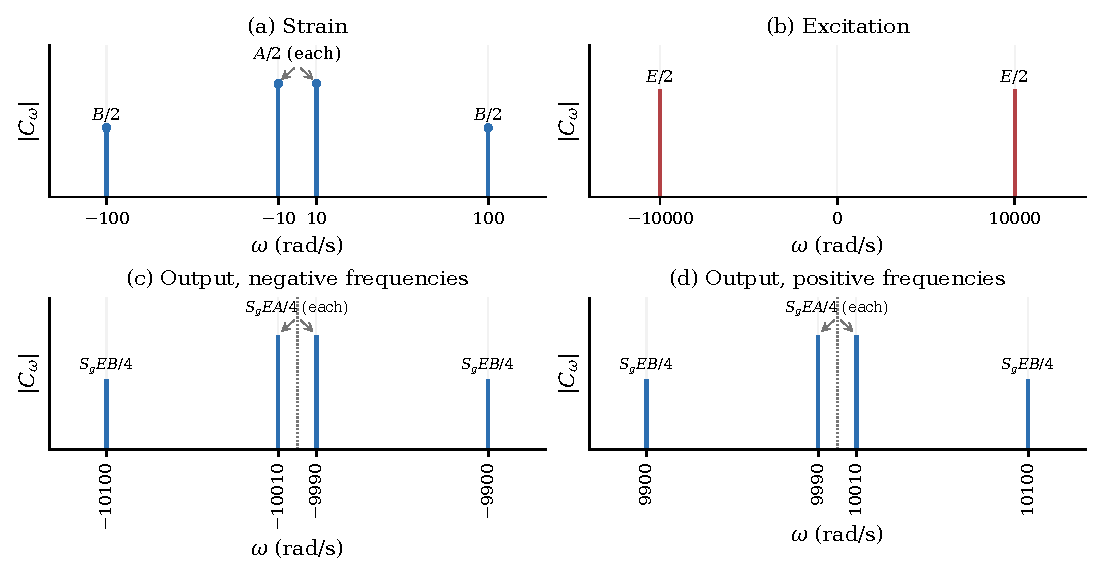
\includegraphics[width=.98\linewidth]{ch5-bridge-spectra.pdf}
\end{center}
图画的是双边复系数的模 $|C_\nu|$，纵向高度按符号示意，精确值见标注；输出正负频率簇分开展示，实际频率位置保持不变。虚线标出载频，虚线位置没有理想谱线。

\textbf{与Hz频谱的换算。}各频率都除以 $2\pi$。激励频率是
\[
f_c=\frac{10000}{2\pi}\approx1591.55\,\mathrm{Hz},
\]
并非 $10\,\mathrm{kHz}$。应变两频率约为 $1.592$、$15.915\,\mathrm{Hz}$，边带相对载频的偏移也分别是这两个数值。

\nt{只给单边峰值谱时，两组输出边带的高度分别为 $|S_gEA|/2$ 与 $|S_gEB|/2$。本题图采用双边复系数模，因此相应高度再减半。无论采用哪一种，都必须说明约定，并保留正弦激励所决定的相位信息。}

\subsection*{本题知识点与公式}\label{kn:5-2}
\noindent\textbf{已学前置：}桥臂接法和全桥系数见\hyperref[kn:5-1]{本章第1题知识讲解}；乘余弦的频移性质见\hyperref[kn:2-6]{第2章第6题知识讲解}；冲激缩放见\hyperref[kn:2-3]{第2章第3题知识讲解}。本题新增交流应变桥的乘法模型、实际桥谱的三种表示对照，以及带参考相位误差的同步解调。

\paragraph{1. 桥路的分压比为何成为调幅系数}
电桥的电源是交流量，并不意味着每个桥臂都必须是电抗。本题桥臂为电阻，若其瞬时电阻由缓变应变确定、导线电容等寄生效应可忽略，原来的电阻分压公式在每个时刻仍成立。设 $k_b$ 为无量纲桥路系数，则
\[
u_y(t)=k_bS_g\varepsilon(t)u_0(t).
\]
等量拉压双臂 $k_b=1/2$，交替全桥 $k_b=1$；单臂 $k_b=1/4$ 仅为小信号近似。$S_g,\varepsilon$ 无量纲，$u_0,u_y$ 单位为V，故系数量纲闭合。若桥臂含电抗、激励频率已使寄生参数显著，就要用交流阻抗桥模型，而不能把此瞬时乘法式当作精确结论。

取 $u_0=E\sin\omega_ct$，令 $K_b=k_bS_gE$，有 $u_y=K_b\varepsilon\sin\omega_ct$。$K_b$ 的单位为V/单位应变。应变控制载波幅值，其变号使输出相对激励反相 $180^\circ$；这正是测量拉、压方向的信息。本题全桥 $K_b=S_gE$，故不能额外再除以4。

记 $\mathcal E(f)=\int_{-\infty}^{\infty}\varepsilon(t)e^{-\iu2\pi ft}\diff t$ 为应变的Hz傅里叶变换（周期信号按广义线谱理解）。

\paragraph{2. 双边带抑制载波的“抑制”指无独立载波线}
设应变频谱限于 $|f|\leq f_m$，载频 $f_c=\omega_c/(2\pi)>f_m$。正弦载波的Hz频谱为
\[
U_y(f)=\frac{K_b}{2\iu}
\left[\mathcal E(f-f_c)-\mathcal E(f+f_c)\right].
\]
正、负载频附近各有一份搬移后的基带谱，每份带有幅值和相位系数；正频率簇占 $[f_c-f_m,f_c+f_m]$。本题应变无直流，因而在 $\pm f_c$ 处无单独谱线，称为双边带抑制载波调幅（DSB-SC）。若应变有直流偏置，该偏置乘载波会产生载频谱线，不能仍断言载波线必为零。

本题 $f_m=100/(2\pi)\,\mathrm{Hz}$，而不是100 Hz；输出所需通带是所有边带的位置范围。实信号的负频率系数为正频率系数的共轭，负频率不表示出现另一套独立的物理振荡。

\paragraph{3. 对本题桥谱统一三种表示}
\hyperref[kn:2-6]{第2章第6题}已经定义傅里叶级数系数。把本题任一周期信号写成
$v(t)=\sum_kC_ke^{\iu\nu_kt}$，其中 $\nu_k$ 为角频率、$f_k=\nu_k/(2\pi)$。同一信号的表示对照为
\begin{center}\small
\begin{tabularx}{\linewidth}{@{}p{2.7cm}X>{\raggedright\arraybackslash}p{2.8cm}@{}}
\toprule
表示法 & 在正频率线的位置与系数 & 本题正弦项 $M\sin\nu_kt$\\
\midrule
复指数线谱 & $\nu_k$ 或 $f_k$ 处画 $C_k$ & $C_k=-\iu M/2$\\
Hz傅里叶变换 & $V_f(f)=\sum_kC_k\delta(f-f_k)$ & 冲激权重 $-\iu M/2$\\
角频率傅里叶变换 & $V_\omega(\omega)=2\pi\sum_kC_k\delta(\omega-\nu_k)$ & 冲激权重 $-\iu\pi M$\\
\bottomrule
\end{tabularx}
\end{center}
两种连续变换的关系是 $V_\omega(\omega)=V_f(\omega/2\pi)$。对冲激代入时必须用
\[
\delta\!\left(\frac{\omega}{2\pi}-f_k\right)
=2\pi\,\delta(\omega-2\pi f_k).
\]
因此“横轴从Hz改成rad/s”若指连续傅里叶谱，冲激权重也出现 $2\pi$；若指把同一组傅里叶级数系数移到角频率坐标，$C_k$ 本身不变。这个因子来自变量缩放，正好对应角频率反变换中的 $1/(2\pi)$。

若 $v$ 是电压，$C_k$ 与单边峰值的单位为V，连续傅里叶变换整体的量纲为 $\mathrm{V\,s}$；冲激箭头标的是权重，不是有限高度的“谱密度”。本题每个输出正弦峰值为 $S_gEA/2$ 或 $S_gEB/2$，所以图中的 $|C_k|$ 分别为其一半，正频率相位为 $-90^\circ$。这同时核对了答案表、频谱图与时域展开，不能只对位置而漏对系数。

\paragraph{4. 同步乘法为什么能恢复应变符号}
用同频参考 $r(t)=B_r\sin(\omega_ct+\theta)$，这里将参考作为无量纲控制量，$B_r$ 为无量纲参考幅值，$\theta$ 为参考相对信号载波的相差；真实电压乘法器还须计入其转换系数。由积化和差，
\[
u_yr=\frac{K_bB_r}{2}\varepsilon(t)
\left[\cos\theta-\cos(2\omega_ct+\theta)\right].
\]
低通除去 $2\omega_c$ 附近的频谱后，
\[
\boxed{v_{\mathrm{LP}}(t)
=\frac{K_bB_r}{2}\cos\theta\,\varepsilon(t)}.
\]
参考同相时恢复有符号的基带；$\theta=90^\circ$ 时有效输出为零；$\theta=180^\circ$ 时输出反号。小相差以弧度计时 $\cos\theta\approx1-\theta^2/2$，会形成比例误差。若参考另有频率偏差 $\Delta\omega$，低频项会乘 $\cos(\Delta\omega t+\theta)$，产生缓慢起伏，不能由固定增益校准消除。

高频副本的最低正频率为 $2f_c-f_m$，因此理想分离要求低通保留 $|f|\leq f_m$，并抑制 $2f_c$ 附近的副本；$f_c>f_m$ 提供了不重叠的条件。实际滤波器还要留过渡带，并满足基带内的幅相精度。普通包络只反映 $|K_b\varepsilon|$，拉压符号丢失；同步参考使这个符号可以保留下来。本题之后第4题将把桥、交流放大、解调和低通合并成整条测量链。

\needspace{11\baselineskip}
\section{第3题：多频调幅波的分量与频谱}
\label{hw:5-3}
\keypoint{复习重点：括号中的直流产生载波，余弦分量各产生一对边带。}

\begin{hwquestion}
已知
\[
x_a(t)=(100+30\cos\Omega t+20\cos3\Omega t)\cos\omega_ct,
\]
其中 $f_c=10\,\mathrm{kHz}$、$f_\Omega=500\,\mathrm{Hz}$。求各分量的频率与幅值，并画出调制信号与调幅波的频谱。
\end{hwquestion}

\subsection*{答案与解析}
把零均值的信息信号记为 $m(t)=30\cos\Omega t+20\cos3\Omega t$，把实际控制载波幅值的量记为 $q(t)=100+m(t)$。二者的区别只有 $q$ 含直流100；称“调制信号”时须明确指哪一个。

\textbf{第一步：展开为五个余弦。}
\begin{align*}
x_a(t)={}&100\cos\omega_ct\\
&+15\cos(\omega_c-\Omega)t+15\cos(\omega_c+\Omega)t\\
&+10\cos(\omega_c-3\Omega)t+10\cos(\omega_c+3\Omega)t.
\end{align*}
因此，$30$与$20$是信息信号的峰值，各自平均分到上下两个边带。

\begin{table}[H]
\centering
\begin{tabular}{@{}c c c@{}}
\toprule
分量 & 频率（$\mathrm{kHz}$） & 时域余弦峰值 \\
\midrule
三倍调制频率的下边带 & $10-1.5=8.5$ & $10$ \\
基频的下边带 & $10-0.5=9.5$ & $15$ \\
载波 & $10$ & $100$ \\
基频的上边带 & $10+0.5=10.5$ & $15$ \\
三倍调制频率的上边带 & $10+1.5=11.5$ & $10$ \\
\bottomrule
\end{tabular}
\end{table}

\textbf{第二步：给出带直流的调制量频谱。}沿用Hz傅里叶变换约定：
\[
Q(f)=100\delta(f)+15[\delta(f-500)+\delta(f+500)]
+10[\delta(f-1500)+\delta(f+1500)].
\]
若画的是 $m(t)$，删去 $100\delta(f)$，其余完全相同。调幅后
\begin{align*}
X_a(f)={}&50[\delta(f-10000)+\delta(f+10000)]\\
&+7.5\!\!\sum_{\nu\in\{9500,10500\}}[\delta(f-\nu)+\delta(f+\nu)]\\
&+5\!\!\sum_{\nu\in\{8500,11500\}}[\delta(f-\nu)+\delta(f+\nu)].
\end{align*}
每条正、负频率线的冲激权重是对应余弦峰值的一半；各系数为正，故相位均为零。

\begin{center}
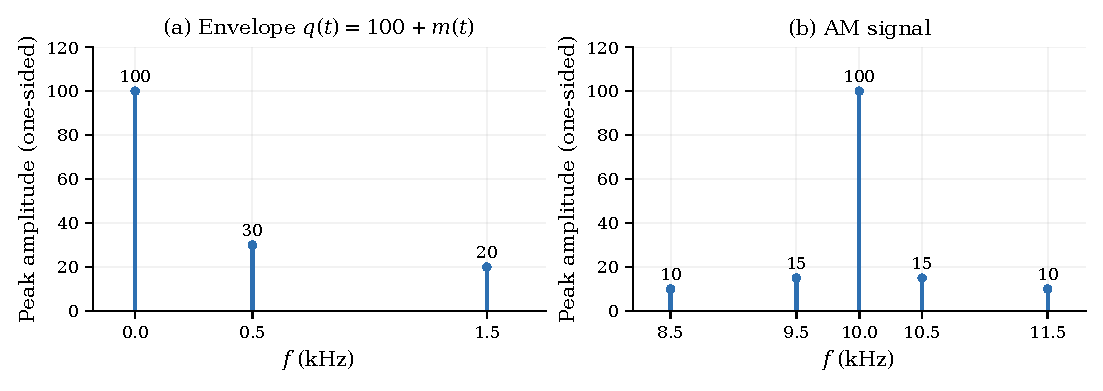
\includegraphics[width=.98\linewidth]{ch5-am-spectra.pdf}
\end{center}
为方便直接读取五个余弦的幅值，本图使用\textbf{单边峰值谱}：正频率余弦项画其峰值，直流画其常数值。若改画双边谱，在正负两侧各画一半峰值；直流仍为100，不做翻倍或减半。

\textbf{第三步：检验包络是否翻折。}由三角不等式，
\[
q(t)\geq100-30-20=50>0.
\]
因而该调幅波无包络翻折，可在适当时间常数与器件工作条件下采用包络检波，检出 $q(t)$ 后再去掉直流100。正频率占用范围为 $8.5\sim11.5\,\mathrm{kHz}$，带宽为 $3\,\mathrm{kHz}=2\times1500\,\mathrm{Hz}$。

\nt{直流100不产生“零频率的射频输出”，而是乘载波后形成 $10\,\mathrm{kHz}$ 谱线。$3\Omega$ 对应 $1500\,\mathrm{Hz}$，不能把它当作 $3\,\mathrm{Hz}$，也不能把两个边带幅值仍写成30、20。}

\subsection*{本题知识点与公式}\label{kn:5-3}
\noindent\textbf{已学前置：}频谱搬移见\hyperref[kn:2-6]{第2章第6题}；本章第\ref{hw:5-2}节已讲DSB-SC和三种线谱约定。本题新增带独立载波的常规调幅、多音调制度、包络检波条件及同阻抗下的功率分配。

\paragraph{1. 常规AM把直流偏置也乘到了载波上}
令零均值信息为 $m(t)$、偏置为 $D>0$，常规AM写成
\[
x_a(t)=[D+m(t)]\cos\omega_ct,\qquad
m(t)=\sum_iM_i\cos(\Omega_it+\theta_i).
\]
$D$ 与 $M_i$ 的量纲相同；若 $x_a$ 为电压，它们以V计。展开后，$D\cos\omega_ct$ 是独立载波，每个调制分量产生
\[
\frac{M_i}{2}\cos[(\omega_c+\Omega_i)t+\theta_i]
+\frac{M_i}{2}\cos[(\omega_c-\Omega_i)t-\theta_i].
\]
此处假设 $\omega_c>\Omega_i>0$。下边带的相位为 $-\theta_i$，上边带为 $+\theta_i$，不能在有初相位时只复制幅值而忽略相位。本题初相位全为0，因此五个余弦分量均可按正峰值直接读谱。

Hz变换中，正频率载波冲激权重是 $D/2$，第 $i$ 组正频率上、下边带的复权重分别为 $(M_i/4)e^{\iu\theta_i}$、$(M_i/4)e^{-\iu\theta_i}$，其模均为 $|M_i|/4$；单边峰值谱则画 $D$ 与 $|M_i|/2$。信息谱本身在 $\pm f_i$ 的复权重为 $(M_i/2)e^{\pm\iu\theta_i}$。搬移的一次减半与双边分解的一次减半各有来源，不能因此丢掉谱线相位。

\paragraph{2. 多音调制度应怎样定义与检查}
单音时定义无量纲调制度 $\mu=|M|/D$。多音可逐项记 $\mu_i=|M_i|/D$，但是否过调取决于总和 $m(t)$ 的实际最小值：
\[
\boxed{D+m(t)\geq0\quad\text{对全部 }t\text{ 成立}}.
\]
一个便于手算的充分条件是
\[
D\geq\sum_i|M_i|\qquad\Longleftrightarrow\qquad
\sum_i\mu_i\leq1.
\]
它利用了三角不等式；相位或频率关系使极小值不能同时出现时，这个条件可以偏保守，不能把“超过此充分界限”一概当作已经证明过调。对多音只检验每个 $\mu_i<1$ 也不充分，因为各项可能同时向下叠加。

本题 $\mu_1=0.3,\ \mu_3=0.2$，且总和为0.5，故 $q(t)=100+m(t)$ 始终为正。理想外包络为 $|q(t)|$；当 $q$ 不变号时，它保留全部调制波形。若 $q$ 变负，外包络会把负部翻上来，丢失有符号的 $q$，造成包络检波失真；已有相干参考时仍可用同步方法恢复，这是解调方式的条件，而非乘法公式失效。

\paragraph{3. 带宽由最高调制频率决定}
当信息频谱占 $|f|\leq f_m$、载频 $f_c>f_m$ 时，正载频附近的边带范围为 $f_c-f_m$ 到 $f_c+f_m$，所需传输带宽为
\[
\boxed{B_{\mathrm{AM}}=2f_m}.
\]
$B_{\mathrm{AM}}$ 与 $f_c$ 均以Hz计，$\omega_c$ 与 $\Omega_i$ 则以rad/s计。本题最高调制频率是 $3f_\Omega=1500\,\mathrm{Hz}$，所以传输带宽为3000 Hz。独立载波线位于此区间中间；它的存在不再额外增加占用带宽。

\paragraph{4. 载波与边带的平均功率从正交性得到}
以下专指 $x_a$ 为电压、作用在同一纯电阻负载 $R_L$ 上、各谱线频率互不重合，且按足够长时间或共同周期求平均。峰值为 $V_p$ 的余弦均方根为 $|V_p|/\sqrt2$，平均功率为 $V_p^2/(2R_L)$。不同频率交叉项平均为零，故载波与全部边带功率分别为
\[
P_c=\frac{D^2}{2R_L},\qquad
P_{\mathrm{SB}}=\sum_i2\frac{(M_i/2)^2}{2R_L}
=\frac{\sum_iM_i^2}{4R_L}.
\]
功率以W计，$R_L$ 以 $\Omega$ 计。总功率与信息边带所占比例为
\[
P_{\mathrm{tot}}=P_c\left(1+\frac12\sum_i\mu_i^2\right),
\qquad
\eta=\frac{P_{\mathrm{SB}}}{P_{\mathrm{tot}}}
=\frac{\sum_i\mu_i^2}{2+\sum_i\mu_i^2}.
\]
这也可由\hyperref[kn:2-6]{第2章第6题的Parseval关系}得到。载波提供包络偏置，却本身不随信息变化；因而常规AM的功率并非全部位于信息边带。单音不过调时 $\mu\leq1$，此模型的最高边带功率比例为 $1/3$。多音不能把 $\sum\mu_i^2$ 直接当作包络极值条件，功率求和与峰值叠加是不同问题。若各频率看到不同阻抗，上式需要逐频率计算真实功率，不能只比较电压平方。

\paragraph{5. 包络检波还需要时间尺度与器件条件}
理想二极管--RC检波器在载波峰附近充电，峰间通过负载放电：时间常数太小会留下明显载波纹波，太大则跟不上下降包络。常用量级条件是
\[
\frac1{\omega_c}\ll\tau_d\ll\frac1{\omega_m},
\qquad \omega_m=2\pi f_m.
\]
$\tau_d$ 单位为s。这只是载波与包络快慢分离的指导式；实际还须检查允许纹波、二极管压降、充电时间及斜切失真。下降包络的局部跟随还要求放电速率不小于包络下降速率，即近似检查
$q/\tau_d\gtrsim|\diff q/\diff t|$。因此即使本题已经证明不过调，也不能跳过检波器动态条件。检出 $q(t)$ 后，去除已知直流 $D$ 并标定增益，才得到零均值信息 $m(t)$。

\needspace{11\baselineskip}
\section{第4题：激励频率与动态应变仪工作频带}
\label{hw:5-4}
\keypoint{复习重点：载频是搬移位置，工作频率是可准确恢复的被测量频带。}

\begin{hwquestion}
某动态应变仪的电桥激励频率为 $10\,\mathrm{kHz}$，工作频率为 $0\sim1500\,\mathrm{Hz}$。用调幅与解调原理解释二者的关系。
\end{hwquestion}

\subsection*{答案与解析}
设应变频谱限于 $|f|\leq1500\,\mathrm{Hz}$，理想桥路输出 $u_y(t)=K\varepsilon(t)\cos(2\pi10000t)$，则
\[
U_y(f)=\frac K2[\mathcal E(f-10000)+\mathcal E(f+10000)].
\]
其中 $\mathcal E(f)$ 为应变频谱，$K$ 含桥路系数、片灵敏系数与激励幅值。因此输出在正载频附近占
\[
\boxed{10000-1500\leq f\leq10000+1500}
\quad\Longrightarrow\quad\boxed{8.5\sim11.5\,\mathrm{kHz}}.
\]
交流放大与带通环节应覆盖整段边带。同步乘以同相 $10\,\mathrm{kHz}$ 参考后，信号一部分回到 $0\sim1500\,\mathrm{Hz}$ 基带，另一部分移到 $20\,\mathrm{kHz}$ 附近。低通保留基带，再作比例标定，便得到应变输出。

所以\textbf{10 kHz是激励载频，1500 Hz是被测应变变化频率的上限}。工作频带受桥路、交流放大、解调和输出低通的整体幅相特性约束，并不是由激励频率直接等同得到。

\textbf{下限为何可为零？}恒定应变会改变载波幅值或相对相位，仍能由同步或相敏检波恢复为有正负的直流输出。只要测量链允许直流基带，就能测静态应变；信息不要求必须以低频电压直接通过全部交流放大级。

\textbf{带宽检查：}两边带共需3000 Hz带宽；输出低通还需在0--1500 Hz内满足精度，不能把1500 Hz直接当作无误差的 $-3\,\mathrm{dB}$ 截止点。

\subsection*{本题知识点与公式}\label{kn:5-4}
\noindent\textbf{已学前置：}频谱搬移与同步解调见\hyperref[kn:5-2]{本章第2题}，包络与有符号信息的区别见\hyperref[kn:5-3]{本章第3题}。本题新增整条动态应变测量链的通带要求，以及载频附近的响应怎样共同决定基带测量精度。

\paragraph{1. 沿测量链追踪同一段信息}
交流供桥的基本链路是
\[
\text{应变}\ \longrightarrow\ \text{交流桥调幅}\
\longrightarrow\ \text{带通放大}\
\longrightarrow\ \text{同步解调}\
\longrightarrow\ \text{输出低通}.
\]
信号在各环节的频谱位置不同，但被测应变的变化频率没有因此变成载频。设应变占 $|f|\leq f_m$，桥输出采用 $K\varepsilon(t)\cos2\pi f_ct$，则正载频附近占 $[f_c-f_m,f_c+f_m]$。本题 $f_c=10\,\mathrm{kHz}$、$f_m=1.5\,\mathrm{kHz}$，因而各环节应检查：
\begin{center}\small
\begin{tabularx}{\linewidth}{@{}p{2.5cm}X@{}}
\toprule
环节 & 需要通过或抑制的频带\\
\midrule
交流桥与交流放大 & 正频率有效边带为 $8.5\sim11.5\,\mathrm{kHz}$，负频率为其镜像；幅相均须满足恢复要求。\\
同步乘法 & 同频参考把有效信息搬回 $|f|\leq1.5\,\mathrm{kHz}$，同时产生 $2f_c$ 附近副本。\\
输出低通 & 保留 $0\sim1.5\,\mathrm{kHz}$，并抑制 $18.5\sim21.5\,\mathrm{kHz}$ 的正频率副本及其负频率镜像。\\
\bottomrule
\end{tabularx}
\end{center}
真实电路还会产生谐波和噪声，表中范围描述理想乘法所需的最低频谱检查。本题不能据此确定实际电路的阶数或允许误差，因为这些指标没有给出。

\paragraph{2. 为什么不能只检查载频处的增益}
把桥后、解调前的线性响应记为 $G(f)$，输出低通记为 $L(f)$，二者均为复数频响。无量纲参考取 $2\cos(2\pi f_ct+\theta)$；系数2专门补偿一次乘余弦的 $1/2$。设带外副本最终被低通除去，则由两次频移直接得到基带等效频响
\[
\boxed{
H_{\mathrm{eq}}(f)=\frac K2 L(f)
\left[e^{-\iu\theta}G(f+f_c)+e^{\iu\theta}G(f-f_c)\right]
},\qquad |f|\leq f_m.
\]
推导要点是：第一次调制产生的两份 $\mathcal E$，经过 $G$ 后分别乘上各自所在频率处的响应；第二次调制把它们都搬到基带，因此\textbf{复数贡献相加}，不能只相加幅值。这一公式假定激励稳定、桥路乘法模型成立、带外副本不与基带重叠，并且参考与载波同频。若参考未乘系数2，整式还要再除以2。

$K$ 的单位为V/单位应变；若其余环节输出、输入都是电压，$G,L$ 为无量纲增益，$H_{\mathrm{eq}}$ 仍是V/单位应变。实系数电路满足 $G(-f)=G^*(f)$，但正载频附近上下边带的增益、相位仍可能不对称；只在 $f_c$ 测一个增益不能知道整个 $H_{\mathrm{eq}}$ 是否平坦。

若边带范围内 $G$ 等效于共同增益与延迟，并通过参考相位校准消除载波传播相移，基带可近似得到一个共同增益和共同延迟。若上下边带的幅相畸变不同，一个参考相位旋钮一般不能补偿全部基带频率。

\paragraph{3. 工作频带、通带指标与截止频率的区别}
“工作频率 $0\sim1500\,\mathrm{Hz}$”应理解为在规定精度下可测的应变变化范围。完整指标还应给允许幅值误差、相位误差或延迟误差。设用直流灵敏度 $H_{\mathrm{eq}}(0)>0$ 标定，并允许共同延迟 $t_d$，可用
\[
\left|\frac{|H_{\mathrm{eq}}(f)|}{H_{\mathrm{eq}}(0)}-1\right|
\leq\epsilon_A,\qquad
\left|\arg H_{\mathrm{eq}}(f)+2\pi ft_d\right|
\leq\epsilon_\phi
\]
检查工作频带内的保真性；相位须先连续展开，$\epsilon_A$ 无量纲，$\epsilon_\phi$ 用rad，$t_d$ 用s。单频幅值测量可能只规定第一项，多频波形测量则不能忽略第二项。

半功率截止点的幅值已经降到参考值的 $1/\sqrt2$，即约29.3\%衰减，通常不等于精密测量的带宽边界。对一阶输出低通，若要求在 $f_m$ 处衰减不超过 $\epsilon_A$，由\hyperref[kn:3-2]{第3章第2题}可直接写出
\[
\tau\leq
\frac{\sqrt{(1-\epsilon_A)^{-2}-1}}{2\pi f_m},
\qquad
f_{\mathrm{cut}}\geq
\frac{f_m}{\sqrt{(1-\epsilon_A)^{-2}-1}}.
\]
所以实际设计需让允许误差内的通带覆盖1500 Hz，并另给过渡带；不能把 $f_{\mathrm{cut}}=1500\,\mathrm{Hz}$ 当作默认答案。第5题将统一讲截止与滤波器的其他频带指标。

\paragraph{4. 交流放大为何仍能测零频率应变}
恒定应变 $\varepsilon_0$ 使桥输出为 $K\varepsilon_0\cos2\pi f_ct$，它是载频处的交流信号，能够通过交流放大级。同步解调后得到与 $\varepsilon_0$ 成正比的直流，因此\textbf{被测量的零频率不需要以直流电压穿过解调前的全部电路}。

要保留直流与符号，必须保证解调参考相位稳定、最终基带链有非零直流增益、后级不再用去直流高通把静态信息删去，并且正负应变的标定一致。按\hyperref[kn:5-2]{第2题}，参考相差会给基带乘 $\cos\theta$：相差 $90^\circ$ 会使有效信号消失，反相会使拉压符号颠倒。实际零点漂移与桥路初始失衡还需单独调零；调零并不等于可以丢掉被测量真实的直流变化。

\nt{本题激励 $10\,\mathrm{kHz}$ 与第2题的 $10000\,\mathrm{rad/s}$ 是不同单位、不同数值；不能把二者直接当作同一个载频。}

\needspace{11\baselineskip}
\section{第5题：截止频率与倍频程判断}
\label{hw:5-5}
\keypoint{复习重点：从 $f_{c2}/f_{c1}=2^n$ 推导，避免把三个不同的根号混淆。}

\begin{hwquestion}
设带通滤波器下、上截止频率为 $f_{c1},f_{c2}$，中心频率为 $f_0$。判断：
\begin{enumerate}
\item 一倍频程滤波器有 $f_{c2}=\sqrt2\,f_{c1}$。
\item $f_0=\sqrt{f_{c1}f_{c2}}$。
\item 截止频率位于幅值相对通带参考值下降约 $3\,\mathrm{dB}$ 的位置。
\item 下限频率相同时，一倍频程中心频率为 $1/3$ 倍频程中心频率的 $\sqrt[3]2$ 倍。
\end{enumerate}
\end{hwquestion}

\subsection*{答案与解析}
本题采用对数对称带通频带和常用半功率截止点约定。

\textbf{（1）错误。}一倍频程的定义是上下限频率之比为2：
\[
\boxed{f_{c2}=2f_{c1}},\qquad
f_0=\sqrt{f_{c1}\cdot2f_{c1}}=\sqrt2\,f_{c1}.
\]
命题把中心与下限之比，误写成上限与下限之比。若上、下限比为 $\sqrt2=2^{1/2}$，相应宽度只有半倍频程。

\textbf{（2）正确。}对数轴上的中点满足
\[
\log f_0=\frac{\log f_{c1}+\log f_{c2}}2,
\]
所以 $f_0=\sqrt{f_{c1}f_{c2}}$，不是算术平均 $(f_{c1}+f_{c2})/2$。该结论使用了本题的中心频率定义。

\textbf{（3）按本题常用约定正确。}半功率点的幅值比是 $1/\sqrt2$，
\[
20\log_{10}\frac{1}{\sqrt2}=-3.0103\,\mathrm{dB}\approx-3\,\mathrm{dB}.
\]
须相对于规定通带参考幅值；它不是绝对电压的分贝读数。采用其他截止指标的滤波器，需使用对应定义。

\textbf{（4）正确。}设共同下限为 $f_L$。一倍频程上限为 $2f_L$，中心为 $2^{1/2}f_L$；$1/3$ 倍频程上限为 $2^{1/3}f_L$，中心为 $2^{1/6}f_L$。故
\[
\boxed{\frac{f_{0,\,1\mathrm{oct}}}{f_{0,\,1/3\mathrm{oct}}}
=2^{1/2-1/6}=2^{1/3}=\sqrt[3]2}.
\]


\subsection*{本题知识点与公式}\label{kn:5-5}
\noindent\textbf{已学前置：}测量精度内的工作频带与截止点的区别见\hyperref[kn:5-4]{本章第4题}；一阶幅相曲线见\hyperref[kn:3-1]{第3章第1题}。本题新增滤波器的完整频带语言、分贝和滚降，以及对数对称带通的中心、品质因子与倍频程关系。

\paragraph{1. 四种滤波器按“允许通过什么”区分}
对线性时不变滤波器，$Y(f)=H(f)X(f)$，$H$ 一般同时改变幅值与相位。对实系数滤波器，实冲激响应保证 $H(-f)=H^*(f)$，负频率响应由此确定，通常只列正频率：
\begin{center}\small
\begin{tabularx}{\linewidth}{@{}p{1.3cm}p{3.2cm}X@{}}
\toprule
类型 & 主要通过范围 & 本章中的联系\\
\midrule
低通 & 从直流到某上边界 & 同步解调后保留应变基带。\\
高通 & 高于某下边界 & 可抑制直流漂移；但不能用于必须保留静态应变的最终基带。\\
带通 & 下、上边界之间 & 在载频附近保留两边带并抑制较远干扰。\\
带阻 & 通过某段阻带以外的频率 & 抑制窄频段干扰；阻带很窄时常称陷波。\\
\bottomrule
\end{tabularx}
\end{center}
滤波能按频率选择成分；有用信号与噪声若处于相同频率，普通线性选频不能只除去噪声而保留该频率的全部信号。需要保留波形时，也不能只画幅频响应而完全不检查相位。

\paragraph{2. 通带、阻带、过渡带与截止点是不同指标}
通带是在规定最大衰减或纹波内通过的范围；阻带是在规定最小衰减下需抑制的范围；两者之间为过渡带。对低通，常用通带边缘 $f_p$、阻带边缘 $f_s$，且 $f_p<f_s$；在阻带要求 $|H|$ 足够小，不要求实际电路严格为零。

“截止频率”必须附定义。本题按半功率约定，以通带参考幅值 $A_{\mathrm{ref}}$ 为基准：
\[
|H(f_c)|=\frac{A_{\mathrm{ref}}}{\sqrt2}.
\]
对一阶低通，这个点也叫转折点；对带纹波的实际滤波器，设计表中的截止、通带边缘、峰值频率可能采用不同指标，不能把所有名称无条件等同。带通的 $f_{c1},f_{c2}$ 须使用同一个参考及同一个幅值标准，才可据此计算一致的带宽。

\paragraph{3. 幅度分贝与功率分贝为什么差一倍}
幅值比 $a>0$ 的分贝表达为 $L_A=20\log_{10}a$，功率比 $p>0$ 的表达为 $L_P=10\log_{10}p$；dB是对数比值，本身不表示绝对电压。若电压作用于同一纯电阻，则 $P=V_{\mathrm{rms}}^2/R$，于是 $p=a^2$，两种表达相等：
\[
10\log_{10}(a^2)=20\log_{10}a.
\]
半功率 $p=1/2$ 对应幅值 $a=1/\sqrt2$，两者均为 $-3.0103\,\mathrm{dB}$。若电压比较两端的阻抗不同，就不能只凭 $a=1/\sqrt2$ 判断功率减半。增益的dB值可为负；若用“衰减量”为正数的写法，则 $A_{\mathrm{dB}}=-20\log_{10}a$，需说明符号约定。

\paragraph{4. 阶次与滚降描述过渡有多快}
对约分后的典型有理系统，阶次对应系统动态状态的数目，通常由分母多项式次数判断。阶次增加可以提高某些滤波器的带外衰减速度，但响应形状还取决于极点、零点及设计类型，不能仅由阶次知道通带纹波和相位。

以分子为常数的 $N$ 阶全极点低通为例，远高于全部转折频率时 $|H|\propto f^{-N}$，故幅值dB的渐近斜率为
\[
-20N\,\mathrm{dB/dec}
\quad\text{或}\quad
-20N\log_{10}2\approx-6.0206N\,\mathrm{dB/oct}.
\]
dec表示频率变为10倍，oct表示频率变为2倍；它们描述\textbf{区间变化的斜率}。在截止附近不能把渐近斜率当作精确衰减。带通两侧、带零点的滤波器和高通的通带端应按各自的分子分母次数分析，不能直接把上述低通斜率套到所有滤波器。

\paragraph{5. 几何中心、绝对带宽与品质因子}
若带通在对数频率坐标上以 $f_0$ 为中心，上、下边界距离相等，则
\[
\log\frac{f_0}{f_{c1}}=\log\frac{f_{c2}}{f_0}
\quad\Longrightarrow\quad
\boxed{f_0=\sqrt{f_{c1}f_{c2}}}.
\]
它是几何平均，而非线性频率轴上的算术中点。绝对带宽、相对带宽和品质因子分别为
\[
B=f_{c2}-f_{c1},\qquad \beta=\frac{B}{f_0},\qquad
Q=\frac{f_0}{B}=\frac1\beta.
\]
$f_0,B$ 单位均为Hz，$\beta,Q$ 无量纲。$Q$ 大表示相对频带窄，并不表示所有误差都更小。对于标准二阶谐振带通，$Q$ 还可与阻尼及能量损耗联系；本题只使用同一半功率边界定义的频带品质因子，不把它任意套到不对称响应或其他截止约定上。

\paragraph{6. 倍频程是对数带宽，不是Hz带宽}
频率从 $f_1$ 变到 $f_2$ 所跨的倍频程数为
\[
n=\log_2\frac{f_2}{f_1}.
\]
因此 $n$ 倍频程带通满足 $f_{c2}/f_{c1}=2^n$。与几何中心联立，
\[
f_{c1}=f_0\,2^{-n/2},\qquad
f_{c2}=f_0\,2^{n/2},\qquad
\boxed{\frac{B}{f_0}=2^{n/2}-2^{-n/2}}.
\]
这些式子不仅给出边界，还说明固定倍频程宽度对应恒相对带宽、恒 $Q$。频率越高，绝对带宽随 $f_0$ 增大；恒Hz带宽则保持 $B$ 不变、相对带宽随中心频率变化。两种滤波器组衡量的是不同的频率分辨尺度。

完整一倍频程取 $n=1$，$1/3$倍频程取 $n=1/3$。本题在相同下限下比较中心，必须先分别求 $f_0=f_{c1}2^{n/2}$，再取比，故得到 $2^{1/3}$；若条件改成相同中心或相同上限，不能继续使用这个结论。这里采用理论二进制倍频程关系，实际仪器的标称中心频率、允差与边缘定义需依其给定规范确认。

\nt{四项判断依次为：错、对、按常用半功率约定对、对。$-3\,\mathrm{dB}$ 使用幅值的 $20\log_{10}$；功率比使用 $10\log_{10}$；同阻抗时，电压幅值比的 $20\log_{10}$ 与功率比的 $10\log_{10}$ 一致。}

\needspace{11\baselineskip}
\section{第6题：双频输入通过一阶低通}
\label{hw:5-6}
\keypoint{复习重点：先计算两个 $\omega\tau$，系统相位差再加到原输入相位上。}

\begin{hwquestion}
已知
\[
H(\iu\omega)=\frac1{1+\iu\omega\tau},\qquad\tau=0.05\,\mathrm s,
\]
输入 $x(t)=0.5\cos10t+0.2\cos(100t-45^\circ)$，求稳态输出，并比较输入、输出的幅相变化。
\end{hwquestion}

\subsection*{答案与解析}
系统静态增益为1，
\[
A(\omega)=\frac1{\sqrt{1+(0.05\omega)^2}},\qquad
\phi(\omega)=-\arctan(0.05\omega).
\]
对 $\omega_1=10\,\mathrm{rad/s}$，有 $\omega_1\tau=0.5$：
\[
A_1=\frac1{\sqrt{1.25}}=0.894427,
\quad\phi_1=-26.5651^\circ,
\]
\[
y_1(t)=0.5A_1\cos(10t+\phi_1)
=0.447214\cos(10t-26.5651^\circ).
\]
对 $\omega_2=100\,\mathrm{rad/s}$，有 $\omega_2\tau=5$：
\[
A_2=\frac1{\sqrt{26}}=0.196116,
\quad\phi_2=-78.6901^\circ.
\]
第二项原相位为 $-45^\circ$，因此输出总相位为 $-123.6901^\circ$：
\[
y_2(t)=0.2A_2\cos(100t-45^\circ+\phi_2)
=0.0392232\cos(100t-123.6901^\circ).
\]
叠加得到
\[
\boxed{\begin{aligned}
y_{\mathrm{ss}}(t)\approx{}&0.447214\cos(10t-26.5651^\circ)\\
&+0.0392232\cos(100t-123.6901^\circ).
\end{aligned}}
\]
常相位用角度标注，数值代入三角函数时应换成弧度。

\begin{table}[H]
\centering\small
\begin{tabular}{@{}c c c c c@{}}
\toprule
$\omega$（$\mathrm{rad/s}$） & 输入幅值 & 输出幅值 & 幅值衰减 & 系统新增相位差 \\
\midrule
$10$ & $0.5$ & $0.447214$ & $10.5573\%$ & $-26.5651^\circ$ \\
$100$ & $0.2$ & $0.0392232$ & $80.3884\%$ & $-78.6901^\circ$ \\
\bottomrule
\end{tabular}
\end{table}

\begin{center}
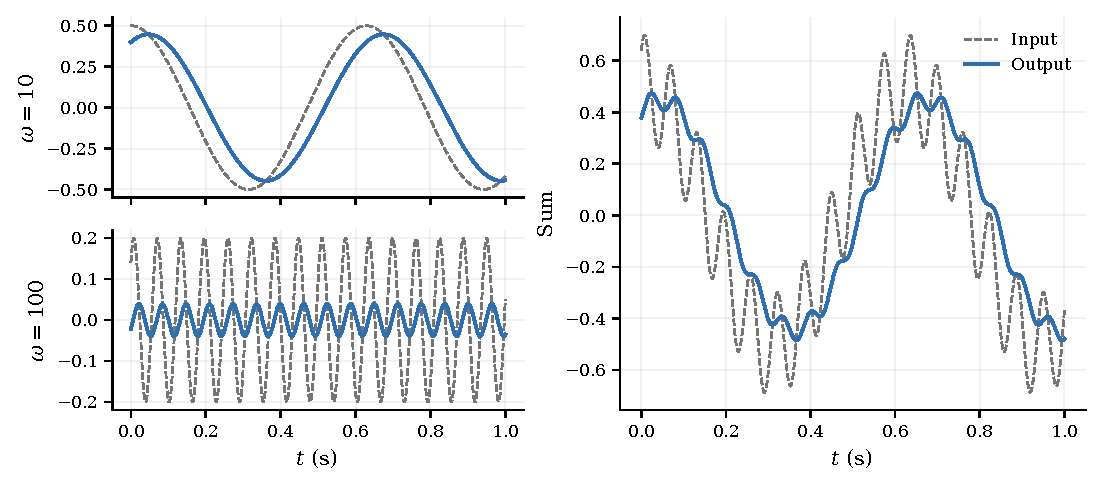
\includegraphics[width=.98\linewidth]{ch5-lowpass-example.pdf}
\end{center}
高频分量被明显抑制，输出主要由低频项决定。高、低频幅值比由 $0.2/0.5=0.4$ 变为约 $0.087706$；各分量相对强弱改变，叠加波形不能只用共同放大与延迟表示。

两分量的等效相位延迟也不同：
\[
t_1=\frac{\arctan0.5}{10}\approx0.046365\,\mathrm s,\qquad
t_2=\frac{\arctan5}{100}\approx0.013734\,\mathrm s.
\]
本滤波器截止角频率 $\omega_c=1/\tau=20\,\mathrm{rad/s}$，截止频率约 $3.1831\,\mathrm{Hz}$。输入高频项处于截止点之上，所以衰减显著。

\subsection*{本题知识点与公式}\label{kn:5-6}
\noindent\textbf{已学前置：}一阶系统的微分方程、传递函数、冲激/阶跃响应和幅相特性见\hyperref[kn:3-1]{第3章第1题}；误差与带宽见\hyperref[kn:3-2]{第3章第2题}；相位延迟、群延迟见\hyperref[kn:3-4]{第3章第4题}。本题保留逐频率解法，新增RC实现、实际加载与级联，以及滤波时如何评价多频保真。

\paragraph{1. 一个RC电路怎样实现题给频响}
理想电压源经电阻 $R$ 接到输出节点，电容 $C$ 从输出接地；输出取电容两端、负载开路。电容阻抗 $Z_C=1/(sC)$，由串联分压，
\[
H(s)=\frac{Z_C}{R+Z_C}=\frac1{1+sRC}.
\]
因此 $\tau=RC$，$R$ 以 $\Omega$ 计、$C$ 以F计、$\tau$ 以s计。本题给出的 $\tau=0.05\,\mathrm s$ 只规定乘积，不能唯一反推出 $R,C$ 各自数值。低频时电容阻抗大、输出接近输入；高频时电容阻抗小、输出被旁路到地，解释了其低通性质。若输出改取电阻两端，频响变为 $sRC/(1+sRC)$，实现高通而非本题模型。

\paragraph{2. 有限负载会同时改变直流增益和时间常数}
若输出端并联纯电阻负载 $R_L$，其等效阻抗为
$Z_p=R_L/(1+sR_LC)$，因此
\[
\boxed{
H_L(s)=
\frac{R_L}{R+R_L}\,
\frac1{1+s(R\parallel R_L)C}
}.
\]
实际直流增益 $K_L=R_L/(R+R_L)$ 小于1，实际时间常数为 $(R\parallel R_L)C$，二者都与未加载结果不同。不能只看到截止频率升高就说测量更准确，因为电压已经先被分压衰减。理想源若有串联内阻 $R_s$，式中驱动电阻应换为 $R+R_s$；若负载还含电容或频率相关阻抗，需重新列网络方程。

要使用本题给定的单位静态增益模型，实际电路须已标定且可用此模型描述，或满足驱动阻抗足够小、负载阻抗远大于所用电阻。电压跟随器等缓冲级以高输入阻抗减小前级加载、以低输出阻抗驱动后级；缓冲器自身带宽与增益误差仍须足够小。

\paragraph{3. 级联后不能沿用单级的截止点}
有缓冲、级间加载可忽略时，总频响是各级复频响的乘积。$N$ 个相同一阶低通级联，
\[
H_N(s)=(1+s\tau)^{-N},\qquad
A_N(\omega)=[1+(\omega\tau)^2]^{-N/2},
\]
\[
\phi_N(\omega)=-N\arctan(\omega\tau).
\]
总幅值相乘、相位相加；它并不等价于把单级 $\tau$ 机械换成 $N\tau$。按总直流增益的半功率点定义截止，解 $A_N=1/\sqrt2$ 得
\[
\boxed{f_{c,N}=\frac{\sqrt{2^{1/N}-1}}{2\pi\tau}}.
\]
$N>1$ 时总体截止低于单级截止。级联虽使高频抑制更强，也会改变通带衰减与相位，所以必须重新核对基带精度。

若两个相同的无源RC低通直接串接、没有缓冲，后一段会加载前一段。设一级节点为 $V_1$、最终输出为 $V_o$，理想电压源为 $V_{\mathrm{in}}$。零初值、最终开路时，节点电流守恒给出
\[
\frac{V_{\mathrm{in}}-V_1}{R}=sCV_1+\frac{V_1-V_o}{R},
\qquad \frac{V_1-V_o}{R}=sCV_o.
\]
由第二式得 $V_1=(1+sRC)V_o$，代入第一式并整理，得到
\[
H_{\mathrm{unbuf}}(s)=\frac1{1+3sRC+s^2R^2C^2},
\]
而非 $(1+sRC)^{-2}$。这个差别说明乘积法的前提是\textbf{各级在实际连接条件下的频响已知}，不是只要画出两个模块就能乘各自空载频响。

\paragraph{4. 多频保真要比较相对幅值和延迟}
设输入为 $\sum_iX_i\cos(\omega_it+\theta_i)$，输出逐项乘 $A_i$、加 $\phi_i$。若目标是保留整个波形，应在有效频带内近似满足
\[
H(\iu\omega)\approx A_0e^{-\iu\omega t_0},
\]
即同一个幅值比 $A_0$ 与同一个延迟 $t_0$，不能只要求每项频率不变。本题高低频幅值比由0.4变为约0.087706，已说明相对强弱明显改变；两个系统新增相位也不对应同一相位延迟。

依\hyperref[kn:3-4]{第3章第4题的延迟定义}，对本题RC直接代入得
\[
t_\phi(\omega)=\frac{\arctan(\omega\tau)}{\omega},
\qquad
\tau_g(\omega)=\frac{\tau}{1+(\omega\tau)^2}.
\]
两者单位为s，求导或计算时相位用rad。前者对应单频相位的等效延迟，后者反映足够窄频带附近包络的传播延迟；不能互相替代。只有 $\omega\tau\ll1$ 时二者都近似 $\tau$。本题 $\omega\tau=0.5$ 与5，相位延迟分别为答案中的0.046365 s与0.013734 s；群延迟则分别为0.04 s与约0.001923 s，也并非常数。

\paragraph{5. 低通的抑噪收益与失真代价}
增大 $\tau$ 会降低截止频率，使高频衰减和相位滞后更强。本题 $\tau$ 是第\ref{hw:3-1}节的10倍；若 $100\,\mathrm{rad/s}$ 分量也属被测信号，输出已不保真。若只提取低频，仍须核查低频项约 $10.56\%$ 的衰减。应先定有用频带与允许幅相误差，再选 $\tau$、阶次和标定；同频干扰不能靠选频滤波无损分离。

\nt{这里 $\tau=0.05\,\mathrm s$，应直接代入本题参数。求的是稳定滤波后的稳态输出，不含启动暂态；若要求从零初始状态接入信号后的全过程，还应依据初始条件补上 $Ce^{-t/\tau}$。}

\chapter*{知识点首次出现索引}
\label{hw:knowledge-index}
\pdfbookmark[chapter]{知识点首次出现索引}{hw-knowledge-index}
\noindent 下表指向每题后的完整知识讲解，不仅指向计算答案。知识在首次出现处展开；后续使用时结合题内“已学前置”回查。题号采用“章号—原题号”，页码可点击跳转。

\begingroup
\setstretch{1.0}
\small
\setlength{\tabcolsep}{5pt}
\begin{longtable}{@{}p{1.05cm}p{12.25cm}r@{}}
\toprule
题号 & 知识点与核心公式范围 & 页码\\
\midrule
\endfirsthead
\toprule
题号 & 知识点与核心公式范围（续） & 页码\\
\midrule
\endhead
\bottomrule
\endfoot
2—1 & 周期、$f$与$\omega$；均值、绝对均值、均方/有效值、方差；峰值与峰峰值、峰值/波形因数；直流和交流均方关系；能量与功率分类。 & \pageref{kn:2-1}\\
2—2 & 复数模、相位、共轭及欧拉公式；傅里叶正反变换、存在条件和谱密度单位；Hz/角频率约定；线性、时移、时标伸缩、共轭对称；能量Parseval关系与指数时间尺度。 & \pageref{kn:2-2}\\
2—3 & 冲激筛选、权重和缩放；主值分布；微分及积分的变换；零频项的确定；常数、复指数、正余弦、阶跃、符号函数的广义变换对。 & \pageref{kn:2-3}\\
2—4 & 频移与时移的区别；卷积定义、冲激卷积及乘积定理；矩形窗、Sa/sinc；主瓣、旁瓣、谱泄漏及观察时长；有符号谱与幅谱。 & \pageref{kn:2-4}\\
2—5 & 单边阻尼振荡的衰减率、包络和振荡周期；复频谱的相位象限；幅谱峰位与名义频率；能量积分、高频尾部及边界光滑性。 & \pageref{kn:2-5}\\
2—6 & 基带/载波/边带/带宽、频带重叠；抑制载波与包络符号；同步解调；傅里叶级数两种形式、正交性、单/双边幅值及周期功率Parseval关系。 & \pageref{kn:2-6}\\
3—1 & LTI与零状态；微分方程、传递函数、冲激响应、卷积和频率响应；相量稳态法；一阶模型、静态增益与时间常数；稳态/暂态及不失真条件。 & \pageref{kn:3-1}\\
3—2 & 幅值误差基准、时间常数不等式；阶跃63.2\%、上升/调节时间；截止频率与精度带宽；Bode幅相渐近；幅值与相位联合设计。 & \pageref{kn:3-2}\\
3—3 & 质量—阻尼—刚度模型；$\omega_n$、$\zeta$与极点；阻尼分类、欠阻尼阶跃/超调/调节时间；二阶幅相与共振峰推导、幅值平坦与低频相位。 & \pageref{kn:3-3}\\
3—4 & 动态灵敏度、静态标定与单频动态校正；按工作频带选择固有频率；相位延迟和群延迟的定义、单位、区别与适用范围。 & \pageref{kn:3-4}\\
4—1 & 应变及电阻定律；应变系数、泊松效应与电阻率变化；方向、温度交叉影响和自热；电流读出、分辨力及电桥读出动机。 & \pageref{kn:4-1}\\
4—2 & 电容三类变参、差动读出；磁阻/自感/互感与差动变压器；复阻抗及交流桥平衡；参数到电压/频率的转换、相敏读出。 & \pageref{kn:4-2}\\
4—3 & 外光电、光导与光伏效应；光谱阈值、响应度和量子效率；光路分类、光电编码与计数；暗信号、饱和和噪声等读出限制。 & \pageref{kn:4-3}\\
4—4 & 洛伦兹力平衡到霍尔电压；霍尔系数、方向与偏置；测磁场/电流/转速的转换链；霍尔式与磁电感应式的静动态区别。 & \pageref{kn:4-4}\\
4—5 & 涡流与趋肤深度、导电性和缺陷取向；压电超声发射/接收、声程、声阻抗与回波；渗透、磁性检测的适用范围和材料限制。 & \pageref{kn:4-5}\\
4—6 & 光纤导光、强度/相位/波长读出；反射式位移传感；膜片压力到光学量的转换；FBG与温度交叉、机械与光电带宽。 & \pageref{kn:4-6}\\
4—7 & 量程与灵敏度；分辨力、准确度、非线性、迟滞、重复性、漂移和交叉敏感；误差基准；加载、后级匹配与完整测量链选型。 & \pageref{kn:4-7}\\
5—1 & 四臂桥路平衡、精确分压与线性化；单/双/全桥的接法、灵敏度和非线性；温度补偿；戴维南等效与负载效应。 & \pageref{kn:5-1}\\
5—2 & 交流应变桥的抑制载波调幅；三种线谱约定的实际换算；同步/相敏解调、参考相位及恢复符号的条件。 & \pageref{kn:5-2}\\
5—3 & 常规AM、调制度及多音包络；边带幅值/权重；同阻抗下的载波与边带功率、效率；调幅带宽与包络检波条件。 & \pageref{kn:5-3}\\
5—4 & 激励载频与被测量工作频带；搬移—放大—解调—低通链；直流基带与极性恢复；各环节通带及整体幅相误差。 & \pageref{kn:5-4}\\
5—5 & 滤波类型、通/阻带、截止点、阶次与滚降；幅值/功率dB；几何中心、分数倍频程、相对带宽和品质因子及约定边界。 & \pageref{kn:5-5}\\
5—6 & 一阶RC实现、负载和缓冲、级联响应；多频幅相比改变；RC相位/群延迟的应用；滤除高频与保持有效信号波形的取舍。 & \pageref{kn:5-6}\\
\end{longtable}
\endgroup


\end{document}
